% The document class supplies options to control rendering of some standard
% features in the result.  The goal is for uniform style, so some attention 
% to detail is *vital* with all fields.  Each field (i.e., text inside the
% curly braces below, so the MEng text inside {MEng} for instance) should 
% take into account the following:
%
% - author name       should be formatted as "FirstName LastName"
%   (not "Initial LastName" for example),
% - supervisor name   should be formatted as "Title FirstName LastName"
%   (where Title is "Dr." or "Prof." for example),
% - degree programme  should be "BSc", "MEng", "MSci", "MSc" or "PhD",
% - dissertation title should be correctly capitalised (plus you can have
%   an optional sub-title if appropriate, or leave this field blank),
% - dissertation type should be formatted as one of the following:
%   * for the MEng degree programme either "enterprise" or "research" to
%     reflect the stream,
%   * for the MSc  degree programme "$X/Y/Z$" for a project deemed to be
%     X%, Y% and Z% of type I, II and III.
% - year              should be formatted as a 4-digit year of submission
%   (so 2014 rather than the accademic year, say 2013/14 say).

\documentclass[ % the name of the author
                    author={Tom Jager},
                % the name of the supervisor
                supervisor={Dr. Daniel Schien},
                % the degree programme
                    degree={MEng},
                % the dissertation    title (which cannot be blank)
                     title={A Bayesian Inference Engine for Calibrating Uncertainty over UMIS Structured MFA Systems},
                % the dissertation subtitle (which can    be blank)
                  subtitle={},
                % the dissertation     type
                      type={research},
                % the year of submission
                      year={2019} ]{dissertation}
\useunder{\uline}{\ul}{}

\begin{document}

% =============================================================================

% This section simply introduces the structural guidelines.  It can clearly
% be deleted (or commented out) if you use the file as a template for your
% own dissertation: everything following it is in the correct order to use 
% as is.

% =============================================================================

% This macro creates the standard UoB title page by using information drawn
% from the document class (meaning it is vital you select the correct degree 
% title and so on).

\maketitle

% After the title page (which is a special case in that it is not numbered)
% comes the front matter or preliminaries; this macro signals the start of
% such content, meaning the pages are numbered with Roman numerals.

\frontmatter

% This macro creates the standard UoB declaration; on the printed hard-copy,
% this must be physically signed by the author in the space indicated.

\makedecl

% LaTeX automatically generates a table of contents, plus associated lists 
% of figures, tables and algorithms.  The former is a compulsory part of the
% dissertation, but if you do not require the latter they can be suppressed
% by simply commenting out the associated macro.

\tableofcontents
% \listoffigures
% \listoftables
% \listofalgorithms
% \lstlistoflistings

% The following sections are part of the front matter, but are not generated
% automatically by LaTeX; the use of \chapter* means they are not numbered.

% -----------------------------------------------------------------------------

\chapter*{Executive Summary}

\noindent
The field of Industrial Ecology (IE) analyses the flow of materials between subsystems and uses a variety of methodologies. The Unified Material Information System (UMIS) is a method for reconciling the most common IE methodologies into a machine readable diagram. As values in IE studies have an inherent uncertainty, it is important to calibrate uncertainty over the entire system under study and include that uncertainty in the results from analysis. Properties of mass balancing can be used to convert IE systems into mathematical models and, statistical approaches can be employed to calibrate the uncertainty of the model parameters. A Bayesian approach using Monte Carlo Markov Chain (MCMC) sampling proposed by Lupton and Allwood provides a way to infer calibrated uncertainty values in Material Flow Analysis (MFA) studies. 

My research hypothesis is that Lupton's approach can be generalised to operate over UMIS diagrams describing MFA studies. The approach will also be extended to handle models involving concentration coefficients and to support the characterisation of uncertainty through normal, log-normal and uniform distributions. The approach is evaluated over a real MFA study using a prototypical stocks and flows database and its correctness is measured against techniques using Gaussian Error Propagation approaches. Whilst this approach is successful it currently lacks full compatibility with all features of UMIS and takes a significant amount of time to complete. Future areas of investigation should focus on incorporating UMIS's treatment of divergent disaggregation, improving the user experience and developing similar approaches for other IE methodologies such as Dynamic MFA and Life Cycle Assessment.

\subsubsection*{Contributions}
\begin{itemize}
    \item Developed a Pythonic implementation of a UMIS diagram
    \item Generalised Lupton's Bayesian Inference approach for uncertainty calibration to operate over MFAs described by UMIS diagrams
    \item Extended Lupton's approach to support observing stock and flow values with log-normal and uniform distributions
    \item Extended Lupton's approach to operate MFA studies that contain composite materials
    \item Implemented a prototype of STAFDB and used it to evaluate my approach over a real MFA case study
\end{itemize}
\begin{comment}
This section should pr\'{e}cis the project context, aims and objectives,
and main contributions (e.g., deliverables) and achievements; the same 
section may be called an abstract elsewhere.  The goal is to ensure the 
reader is clear about what the topic is, what you have done within this 
topic, {\em and} what your view of the outcome is.

The former aspects should be guided by your specification: essentially 
this section is a (very) short version of what is typically the first 
chapter.  Note that for research-type projects, this {\bf must} include 
a clear research hypothesis.  This will obviously differ significantly
for each project, but an example might be as follows:

\begin{quote}
My research hypothesis is that a suitable genetic algorithm will yield
more accurate results (when applied to the standard ACME data set) than 
the algorithm proposed by Jones and Smith, while also executing in less
time.
\end{quote}

\noindent
The latter aspects should (ideally) be presented as a concise, factual 
bullet point list.  Again the points will differ for each project, but 
an might be as follows:

\begin{quote}
\noindent
\begin{itemize}
\item I spent $120$ hours collecting material on and learning about the 
      Java garbage-collection sub-system. 
\item I wrote a total of $5000$ lines of source code, comprising a Linux 
      device driver for a robot (in C) and a GUI (in Java) that is 
      used to control it.
\item I designed a new algorithm for computing the non-linear mapping 
      from A-space to B-space using a genetic algorithm, see page $17$.
\item I implemented a version of the algorithm proposed by Jones and 
      Smith in [6], see page $12$, corrected a mistake in it, and 
      compared the results with several alternatives.
\end{itemize}
\end{quote}
 
\end{comment}


\chapter*{Supporting Technologies}

\begin{itemize}
    \item I used the Pymc3 \cite{salvatier2016probabilistic} Python package for:
    
    \begin{itemize}
        \item Construction of a mathematical model in terms of stochastic and observed stochastic random variables
        \item MCMC sampling from the mathematical model using the NUTS sampler
    \end{itemize}
    
    \item I used the Theano \cite{al2016theano} Python package to perform operations on values sampled from random variables to calculate dependent stock and flow values
    
    \item I used the Seaborn \cite{michael_waskom_2017_883859} and Matplotlib \cite{Hunter:2007} Python packages to plot kernel density estimations of the posterior distributions of parameter values
    
    \item I used Pandas \cite{mckinney-proc-scipy-2010} to read and write records from CSV files in my prototype implementation of STAFDB
    
    \item I used Jupyter Notebook \cite{kluyver2016jupyter} to perform testing of the Bayesian inference engine
 
\end{itemize}
\begin{comment}
{\bf A compulsory section, of at most $1$ page}
\vspace{1cm} 

\noindent
This section should present a detailed summary, in bullet point form, 
of any third-party resources (e.g., hardware and software components) 
used during the project.  Use of such resources is always perfectly 
acceptable: the goal of this section is simply to be clear about how
and where they are used, so that a clear assessment of your work can
result.  The content can focus on the project topic itself (rather,
for example, than including ``I used \mbox{\LaTeX} to prepare my 
dissertation''); an example is as follows:

\begin{quote}
\noindent
\begin{itemize}
\item I used the Java {\tt BigInteger} class to support my implementation 
      of RSA.
\item I used a parts of the OpenCV computer vision library to capture 
      images from a camera, and for various standard operations (e.g., 
      threshold, edge detection).
\item I used an FPGA device supplied by the Department, and altered it 
      to support an open-source UART core obtained from 
      \url{http://opencores.org/}.
\item The web-interface component of my system was implemented by 
      extending the open-source WordPress software available from
      \url{http://wordpress.org/}.
\end{itemize}
\end{quote}
 
- Pymc3
- Theano
- Seaborn
- Pandas
\end{comment}

% -----------------------------------------------------------------------------

\chapter*{Notation and Acronyms}

\noindent
\begin{tabular}{lcl}
CC                 &:     & Concentration Coefficient
  \\
ERD                &:     & Entity Relationship Diagram
   \\
IE                 &:     & Industrial Ecology                                         \\
IOA                &:     & Input Output Assessment
  \\
LCA                &:     & Life Cycle Assessment
  \\
MAP                &:     & Maximum A Posteriori
 \\
MC             &:      &  Monte Carlo
  \\
MCMC             &:      &  Markov Chain Monte Carlo
  \\
MFA                &:     & Material Flow Assessment
  \\
pdf             &:       & Probability density function
 \\
STAF               &:     & Stocks and Flows
 \\
STAFDB             &:      &  Stocks and Flows Database
  \\
  STAFDB-P             &:      &  Stocks and Flows Database-Prototype
  \\
TC                 &:     & Transfer Coefficient
 \\
UMIS               &:     & Unified Materials Information System
  \\

YSTAFDB            &:     & Yale Stocks and Flows Database
  \\

\end{tabular}


% -----------------------------------------------------------------------------

\chapter*{Acknowledgements}
\begin{comment}
{\bf An optional section, of at most $1$ page}
\vspace{1cm} 

\noindent
It is common practice (although totally optional) to acknowledge any
third-party advice, contribution or influence you have found useful
during your work.  Examples include support from friends or family, 
the input of your Supervisor and/or Advisor, external organisations 
or persons who  have supplied resources of some kind (e.g., funding, 
advice or time), and so on.
 
\end{comment}

% =============================================================================

% After the front matter comes a number of chapters; under each chapter,
% sections, subsections and even subsubsections are permissible.  The
% pages in this part are numbered with Arabic numerals.  Note that:
%
% - A reference point can be marked using \label{XXX}, and then later
%   referred to via \ref{XXX}; for example Chapter\ref{chap:context}.
% - The chapters are presented here in one file; this can become hard
%   to manage.  An alternative is to save the content in seprate files
%   the use \input{XXX} to import it, which acts like the #include
%   directive in C.

\mainmatter

% -----------------------------------------------------------------------------

\chapter{Contextual Background}
\label{chap:context}

\noindent
\section{Industrial Ecology}

Industrial ecology (IE) is an area of research focused around the flow of material, energy or money through a system. It can also be described as socio-economic metabolism (SEM) as it models the production, consumption and storage of resources by society. It primarily focuses on the relationship between human originating sectors and the natural ecosystem by modelling industrial infrastructures as their own subsystems that interact with their environment \cite{tibbs1992industrial}. As such it is a multi-disciplinary field which seeks to account for material and energy data and use it to inform social and economic policy as well as business strategy. The primary motivator for Industrial Ecology is to encourage and ensure sustainable development. By most agreed definitions, this involves ensuring that the economical and societal growth occurs without hampering the ability of development in the future \cite{robert2005sustainable}. Therefore research in Industrial Ecology focuses on decoupling the relationship industrial development has on natural ecosystems. To do this, life cycles of products and materials are analysed in order to find areas for greater efficiency and reduced reliance on natural resources. Studies in Industrial Ecology can focus on identifying the amount of flow of specific materials from the anthroposphere into the environment \cite{rockstrom2009safe}, to assessing where new stocks of materials are accumulating \cite{müller2014modeling}, or finding energy and material "loops" which can be closed in order to reuse waste material and energy\cite{esty1998industrial}.

\subsection{Industrial Ecology Methodology}
There exist a variety of different methodologies for studies in Industrial Ecology. The data resulting from IE studies is therefore published in different formats. The three most prevalent methods are Life Cycle Assessments (LCAs), Input-Output Analysis (IOA) and Material Flow Analysis (MFA) \cite{myers2019unified}.

Life Cycle Assessments follow the environmental impact of a product system throughout its life cycle \cite{ISO14040}. It often involves compiling an inventory analysis where the life cycle is modelled as a system of processes with material or energy flowing between them. Inputs and outputs from each process are specified, with special interest paid to flows into and from the environment. This is used to assess the impact of a product and provide information for decision making in order to improve efficiency and reduce negative environmental effects. LCAs have been known to have sector wide impacts through industry collaboration \cite{mattila2012methodological}. Open data formats such as EcoSpold and ILCD as well as shared databases such as EcoInvent \cite{wernet2016ecoinvent}, make this possible as different industry partners can combine research and also easily recreate results to ensure accuracy. 

Input-Output Analyses takes an economic approach to IE and tracks the flow of money between entities in a geographic region. These can then be used to allocate environmental impact to these entities. As economic data on inter-sector flows are generally more granular than data on the movement of physical material, it can be useful to apply data from IOAs in studies that use other methodologies \cite{chen2016building}.

Material and Energy Flow Analyses maps the movement of a specific material(s) or energy in a system, paying particular attention to where it accumulates in the form of stocks. It does this by modelling a system as a collection of processes with material or energy flowing between them or being stored in them. This is useful for identifying where cycles can be created and improved in order to increase recycling and therefore reduce a system's dependence on its environment \cite{müller2014modeling}. Static MFAs are where the scope of the analyses falls over a single specified time-frame, whilst dynamic MFAs use data about past and present quantities to estimate future impacts. This can highlight which resources may become scarce in the future and provide warnings about future environmental impacts.

\section{Unifying Industrial Ecology}
Whilst some studies have incorporated data from one methodology into another \cite{chen2016building}, there is a need to provide a common framework for all varieties of IE data. In \cite{pauliuk2015general}, Pauliuk et al. performed a comprehensive analysis on the different methodologies present in IE. They discovered that each methodology described the system using a shared structure, that of a bipartite directed graph. The shared common property between each system is that material is \textit{transformed} in one process and then \textit{distributed} in a subsequent process. Edges in this bipartite graph denote a flow of material from one a \textit{distribution} node to a \textit{transformation} node or vice versa.

\subsection{STAFDB and UMIS}
Over the past 20 years, the Graedal research group at Yale University have compiled Industrial Ecology data on over 100 materials on a variety of spacial and temporal scales. The data from these studies has been extracted and used to create the Yale Stocks and Flows Database (YSTAFDB) \cite{ystafdb}. Ongoing work by Myers, Hoekman and Petard (to be published), is in developing a community driven database for this data called the Stocks and Flows Database (STAFDB). This is an improvement on YSTAFDB as it is designed to be more user friendly and deals with the problem of divergent disaggregation.

Disaggregation is where a property of data (e.g a process that data is coming from or the material being described) is divided into components. In a broad example, data about cars could be disaggregated into electric and non-electric vehicles or large and small cars. If data from two studies with different techniques of disaggregation (or divergent disaggregation) on the same data were structured into the same system, data could be counted twice when performing analysis \cite{myers2019unified}. To prevent this, process and material data in STAFDB contains a parent field and an \texttt{is\_separator} flag which serves to keep track of methods of disaggregation and prevent double counting.

Myers et al. have created UMIS, the Unified Materials Information System \cite{myers2019unified} as a format to structure data contained in STAFDB. UMIS structures stocks and flows data that comprise IE studies into a UMIS diagram. This method is agnostic to IOA, MFA and LCA methodologies. This diagram is both human and machine readable which allows for greater automation when dealing with stocks and flows data.

UMIS is a step in shifting industrial ecology towards a more virtual platform where industrial ecological data can be stored in a centralised knowledge base, with an ecosystem of tools and routines to develop models and analyse the data for further studies. This would reduce the time taken to perform further studies, allow of greater collaboration in the field and provide greater transparency on results \cite{hertwich2018nullius}. An example of such a platform is the Metabolism Of Cities project, a digital research lab created by Paul Hoekman \cite{MetabolismOfCities}. The platform's primary aim is to encourage research and allow collaboration in studying the metabolism of resources and energy surrounding specific regions. It contains a store of publications, IE data and an online material flow analysis tool to allow users to easily conduct MFA studies and interface with a common online database. Work is currently being done to integrate Metabolism of Cities with STAFDB to allow for future research to be directly inserted into the database. 

\subsection{UMIS Terminology}
The components and design of a UMIS diagram are drawn from MFA concepts but can still be reconciled with IOA and LCA data. A definition list for the components of a UMIS diagram can be found in table \ref{umis_terms}.

\begin{table}[h]
\begin{tabular}{|l|l|}
\hline
{\textbf{UMIS Component}}   & {\textbf{Definition}}                                                                                                                                                                                                                                          \\ \hline
System Boundary        & \begin{tabular}[c]{@{}l@{}}Definition of the boundary of the data. This is defined by the reference\\ space, time-frame and material. Provides a limit of what parts of the real\\ world are being modelling in this system\end{tabular}   \\ \hline
Reference Space        & \begin{tabular}[c]{@{}l@{}}The geographical space within which all processes, stocks and flows\\ internal to the UMIS diagram reside.\end{tabular}                                                                                                        \\ \hline
Reference Material     & \begin{tabular}[c]{@{}l@{}}The material whose stocks and flows are described in the diagram.\end{tabular} \\ \hline
Reference Time frame   & The time-frame over which material is flowing or is stocked.                                                                                                                                                                                              \\ \hline
Process                & An event involving a material                                                                                                                                                                                                                             \\ \hline
Transformation Process & A process where an object is transformed into another object                                                                                                                                                                                              \\ \hline
Distribution Process   & A process where an object is transferred to another process or location                                                                                                                                                                                   \\ \hline
Storage Process        & A process where material is moved into or from storage                                                                                                                                                                                                    \\ \hline
Stock                  & Movement of material between a process and storage                                                                                                                                                                                                        \\ \hline
Flow                   & \begin{tabular}[c]{@{}l@{}}Movement of material between a transformation and distribution process\\ inside the diagram\end{tabular}                                                                                                                       \\ \hline
Cross boundary flow    & \begin{tabular}[c]{@{}l@{}}Movement from material outside the diagram to an internal transformation\\ or distribution process.\end{tabular}                                                                                                               \\ \hline
\end{tabular}
\caption{Components of a UMIS diagram}
\label{umis_terms}
\end{table}

A UMIS diagram can be thought to consist of three layers, processes and flows, virtual reservoir, and meta-data layer. The processes and flows layer builds on the work of Pauliuk in \cite{pauliuk2015general}, and structures the system as flows between transformation and distribution processes in the form of a bipartite directed graph. The virtual reservoir lies on top of this graph and contains information relating to stock. When material is moved in or out of storage in a system, it is represented by moving into or out of the virtual reservoir. As processes represent physical locations in a system, stock are only positioned on top of existing processes. The meta-data layer is used for storing additional information about stocks flows and processes. This is information concerning the reference space or time-frame of a component, source of the data, uncertainty around a quantity's value, unit of the value, calculation details e.t.c. A visualisation of the key aspects of a UMIS diagram can be seen in figure \ref{fig:umis_aspects}. In order to ensure that UMIS diagrams are able to be computer generated, transformation processes are enforced to have only one outflow to a distribution process. If a system's design indicates a flow from a transformation process to multiple distribution processes, the processes must be further disaggregated to separate them. 

\subsubsection{UMIS's Approach to Divergent Disaggregation}
UMIS also deals with the divergent disaggregation problem present in processes and materials. This is done by assigning every process and material a parent field and an \texttt{is\_separator} flag. The parent field contains the process or materials at the next higher level of aggregation. For example the parent field for a blue car material would be car. As a result the processes and materials stored by STAFDB form a tree structure with the \texttt{is\_separator} flag present on edges in the tree to detect divergent disaggregation. This thesis focuses on the relationship between flows and processes and therefore considerations about disaggregation are out of scope, but it is likely that the approach developed will be extendable to navigate the aggregation tree and ensure that divergent disaggregation does not occur within a UMIS diagram.

\begin{figure}[]
\centering
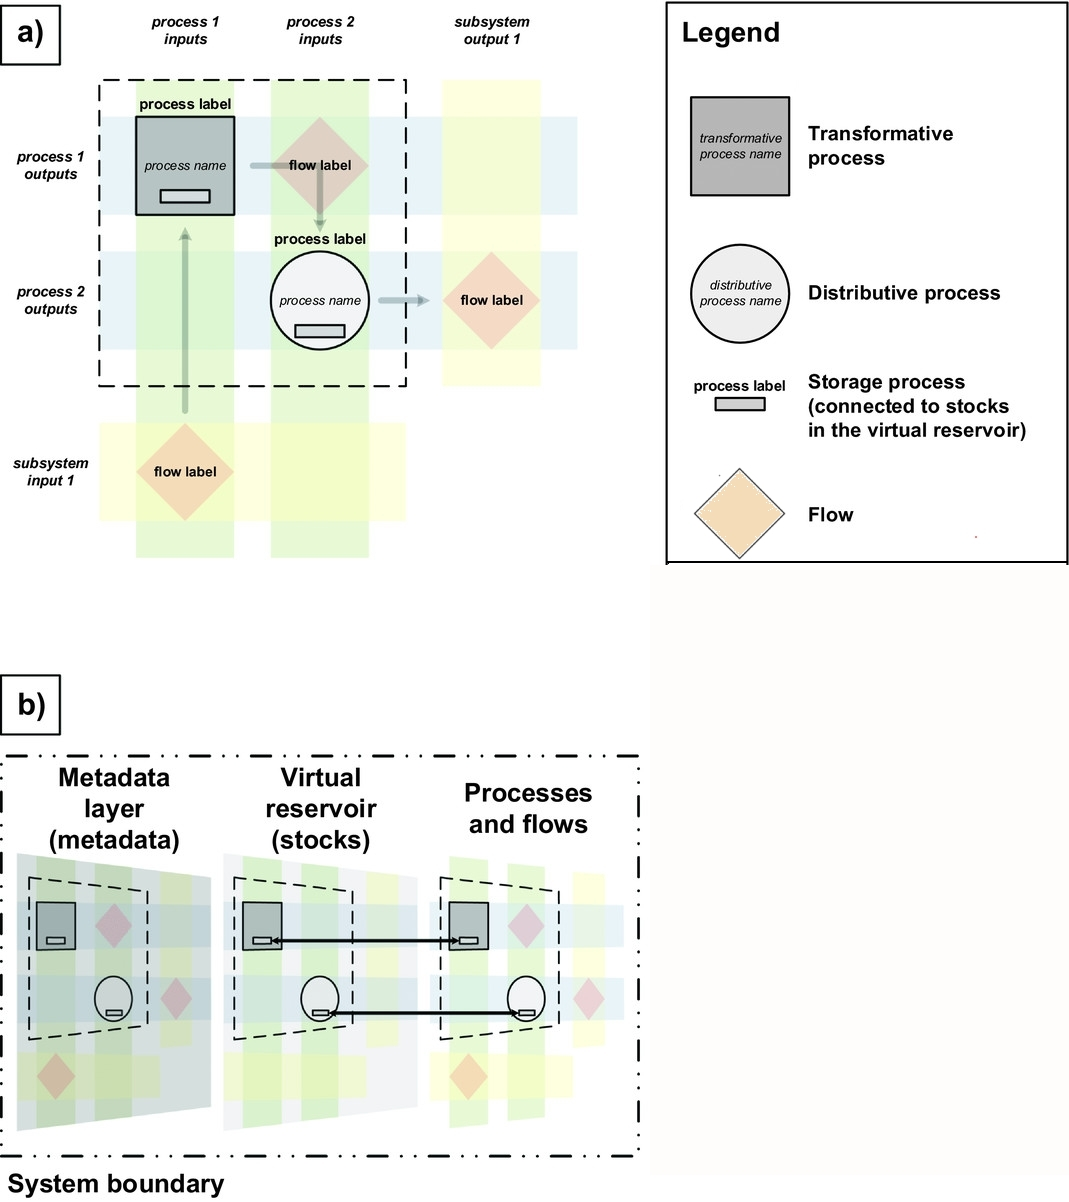
\includegraphics[width=\textwidth]{images/umis_aspects.jpg}
\caption{(a) Key aspects of a UMIS diagram, visualising it in a matrix style. Contains transformation, distribution and Storage processes as well as 3 flows. The processes lie on the diagonal and the flows are on the row of the origin process and the column of the destination process (b) The orientation of the virtual reservoir and meta-data layer in reference to processes and flows. Flows depicted by grey arrows in (a) and conceptual linkages denoted by black arrows in (b) are for illustration and are not properties of UMIS diagrams. UMIS = Unified Materials Information System. Source: \cite{myers2019unified}}
\label{fig:umis_aspects}
\end{figure}

\subsection{Mass Balancing}
\label{sec:mass_balance}
MFA, IOA and LCA all share core modelling concepts. Each methodology involve a separation of background and foreground systems, with the background system acting as a generic supplier of inputs and outputs to the more detailed foreground system \cite{pauliuk2016prospective}. The foreground system is often modelled through a system of equations and constraints, but one concept common to all methodologies is that of mass balancing. The idea of this is that throughout the entire system, matter must be conserved. Therefore the total mass of a given material entering a process must be equal to the total mass leaving \cite{brunner2004practical}. This is defined by the following equation:

\begin{equation}
    \label{eq:mass_balance_1}
    \forall i \; \; \; \;  q_i + \sum^{n}_{j}f_{ji} = \sum^{n}_{j}f_{ij} + o_{i} + \Delta s_i 
\end{equation}

where $i,j \in \{1,..,n\} $ are the processes in the system, $f_{ij}$ is a flow from process $i$ to $j$, $q_i$ and $o_i$ are the inflow and outflow between process $i$ and the background system, and $\Delta s_i$ is the stock being supplied to or coming from storage:     


Further equations can be supplied containing transfer coefficients (TCs). These allocate the total amount of material flowing into the process to each flow leaving the process. This is defined as:

\begin{equation}
    \label{eq:mass_balance_2}
    z_i = q_i + \sum^{n}_{j}f_{ji} + s_i
\end{equation}

\begin{equation}
    \label{eq:mass_balance_3}
    f_{ij} = z_{i}a_{ij}
\end{equation}

where $a_{ij}$ is the transfer coefficient of the flow from process $i$ to $j$, $s_i$ is stock coming from storage (which may be 0) and $z_i$ is the total of all material entering process $i$.

Concentration equations can also be used when stocks and flows deal with composite materials. For example, in a system modelling the flow of iron, a flow may represent the movement of iron oxide ore. This is denoted by the following equation:

\begin{equation}
    \label{eq:mass_balance_4}
    f_s = f_g c_{sg}
\end{equation}

where $f_s$ is the flow of substance $s$ (e.g iron oxide ore), $f_g$ is the amount of good $g$ (e.g iron) in that flow and concentration coefficient (CC) $c_{sg}$ is the concentration of good $g$ in substance $s$.

Whilst Myers et al. have demonstrated how systems from LCA, MFA, IOA studies can be visualized as UMIS diagrams \cite{myers2019unified}, no one has yet used UMIS structured data in a computational model. The approach in this paper demonstrates UMIS's suitability for structuring stocks and flows data for computation.

\section{Uncertainty in IE}
\subsection{What is Uncertainty?}
Common practice in IE research is to first define a system in terms of stocks, flows and processes and then identify values for the stock and flow quantities. These observed values are not always precise and therefore have an inherent uncertainty. As IE studies can be used to guide economic and political decisions, it is important to incorporate this uncertainty when calculating the results. A study by Danius and Burstr\"om \cite{danius2001regional} found that initial conclusions drawn in an MFA study on nitrogen were inconclusive when data uncertainties were taken into account. Therefore in cases where a comparison of values are being conducted, the uncertainty must must be considered to ensure that the results found are significant and cannot be attributed to variation in underlying data. As such, uncertainty is an important and well studied topic in the fields of LCA, IOA and MFA \cite{temursho201712, laner2014systematic, heijungs2004review}.

The sources of uncertainty can be separated into two kinds \cite{ferson1996different}. The first is aleatory uncertainty which comes from random properties in the underlying value. This is where either the method of measuring the value has an uncertainty around it so the precise value is unknown, or the value itself is non-deterministic. The second kind is epistemic which refers to generalisations about the value. One cause can originate from when values vary over space and time, therefore the value for a time period (e.g one year) or a geographic area (e.g the entire UK) can have an associated uncertainty. Another source can be subjective judgement such as when an unknown value is estimated based on a known value. Other causes can include scientific disagreement over the true value of a quantity, imprecise language on what the quantity refers to (e.g an amount being said to be mostly carbon), and approximation in parameters in order to describe the system as a mathematical model. Epistemic uncertainty is potentially reducible through further investigation, however it is sometimes impractical to do so \cite{laner2014systematic}.

Further forms of epistemic uncertainty can be caused by possibilities in how the system is defined or described, however as we are looking at a general algorithm for propagating uncertainty in systems, this can be seen as out of scope. Instead, we will focus on uncertainty in specific parameter values.

\subsection{Incorporating Uncertainty into UMIS}
\label{sec:incorporating_uncertainty}
In \cite{laner2014systematic}, Laner et al. describe the following five step procedure for incorporating uncertainty into MFA studies:

{\setstretch{1}
\begin{enumerate}
    \item Establish mathematical model
    \begin{enumerate}
        \item Define system elements and relationships between the elements
        \item Define equations based on mass balance principle
    \end{enumerate}
    
    \item Characterise data uncertainty
    \begin{enumerate}
        \item Evaluate information about data (model parameters, inputs and outputs)
        \item Define characterising functions for uncertainty
    \end{enumerate}
    
    \item Combine data and mathematical model
    \begin{enumerate}
        \item Balance model and cross-check data
        \item Evaluate plausibility and reconcile data (iterative)
        \item Produce a calibrated model using all available data
    \end{enumerate}
    
    \item Calculate uncertainty for calibrated model
    \begin{enumerate}
        \item Propagate uncertainty through the model and calculate uncertainty of stocks and flows
        \item Interpret uncertainty estimates for resultant values from model 
    \end{enumerate}
    
    \item Analyze sensitivity \& develop scenarios
    \begin{enumerate}
        \item Identify critical model parameters
        \item Change parameters to perform scenario analysis
    \end{enumerate}
\end{enumerate}
}
% 
As MFA, IOA and LCA all share constraints surrounding mass balancing in their system structure, steps 1-4 in the above procedure can be applied to all three methodologies. Where they diverge is in the fifth stage, where the model is used to calculate further values and perform analysis on the system. Therefore providing support for stages 1-4 can be seen as a relevant and useful addition to UMIS and STAFDB.

UMIS provides a method for structuring stocks and flows data into the system as in step one of this procedure. It does not, however, explicitly specify a unified way for specifying how the uncertainty around data values must be described. Current development on STAFDB and in the Metabolism of Cities project favours an approach investigated by Laner in \cite{laner2016novel}. This strategy combines the use of a pedigree matrix to classify data quality, as defined by Weidema and Wesnaes \cite{weidema1996data}, and the application of data quality to uncertainty by Hedbrandt and S\"orme \cite{hedbrant2001data}. The pedigree matrix provides five criteria of data quality (reliability, completeness, temporal correlation and geographical correlation). When a data point is recorded it is given a score for each criteria. The score is combined with a sensitivity level to provide a coefficient of variation. The data point can then be modelled as a normally distributed random variable with a standard deviation related to its coefficient of variation. As stock and flow values can never be negative and can have asymmetrical properties, it is sometimes appropriate to model the data point as a log-normal random variable. Therefore Laner also provides a method for characterising data quality with an uncertainty factor which relates to the standard deviation of a log-normal distribution. Therefore Laner's work could be used to convert descriptions of a data point's uncertainty from quality scores to normal or log-normal probability density functions.

Whilst the above approach provides a method for characterising the uncertainty of individual data points independently, it does not provide support for considering them in respect to the entire system. This is key to steps 3 and 4a of the above procedure. To do this the data must be arranged as a mathematical model and the uncertainties of each model parameter must be calculated under the mass balance constraints. Typically this is performed using statistical approaches through either possibilistic methods, probabilistic methods or sensitivity analysis. 

As a single UMIS diagram structures an IE system, a useful addition to UMIS would be to provide a program to calibrate uncertainty over a UMIS diagram and infer unknown stocks, flows and transfer coefficients. Programs to support analysis such as in steps 4b, and 5 or in situations unique to IOA and LCA would have to be unique to the study and therefore are out of scope for this thesis.

\section{Aims}
The aims for this dissertation are as follows:

\begin{enumerate}
    \item Investigate literature in dealing with uncertainty in MFA models
    \item Develop an approach for creating a mathematical model from UMIS structured data and calibrate uncertainty over it
    \item Add support for representing uncertainty through normal, log-normal and uniform distributions
    \item Evaluate the accuracy and performance of this approach
\end{enumerate}
\begin{comment}

Uncertainty
    - Why is it important to show uncertainty?
        - 
    - What are the methods for showing uncertainty?
    - Why is it important to hav a flexible method for showing uncertainty?
    - Need to show uncertainty
        - All studies are used to inform decision making
        - As such uncertainty has been the subject of various literature reviews in the fields of IOA, MFA and LCA, cite cite cite
        - Impairs reliability
        - Important when considering results
        - Can determine if results are significant compared to uncertainty
        - Environmental impacts and indicators are often calculated directly from    values, need to have accurate uncertainty around those values in order to   confidently talk about environmental impact
    - Sources of uncertainty
        Because IE studies often work on an average (i.e average amount of copper, average amount of zinc flowing through)
        
        read this one, take notes, read the lca one quickly, take notes, see how IOA one is important
    - Methods of dealing with and calculating uncertainty
        - Talk about 2 things that aren't related to probabilistic
        - Talk about the Fuzzy set theory, sensitivity analysis, stan, probabilistic and then lupton and then say where mine fits in 
    - Reliability scores (talk in regards to STAFDB and UMIS, ecoinvent scores)
        - Useful when integrating data from across studies
        - Need for lognormal
        - Need to ensure that consistency is kept according to the later laner paper
  
 - Transformation processes have only one outflow
 - Visualized here as a matrix
- Metabolism of Cities
    - Digital research lab created by Paul Hoekman designed to store and facilitate Industrial Ecology research.
    - Contains a store of publications, IE data and an online material flow analysis tool that is designed to allow users to easily conduct MFA studies and interface with an online database.
    - Its primary aim is to encourage and allow collaboration between researches to fully undertand the metabolism of resources and energy surrounding specific regions.
    - Current
- Industrial Ecology
    What is it
    What methods does it use
        LCA
        IOA
        MFA
- STAFDB
   - over the past 20 years the graedal research group at yale university have compiled Industrial Ecological data covering over 60 chemical elements and over 100,000 data entries
   - The data from this has been extracted and placed into YSTAFDB, currently work is continuing to develop STAFDB, a community driven database that enhances YSTAFDB by making it more user friendly and dealing with problems related to divergent disaggregation.
   Disaggregation is where a classification of data is separated into its constituent parts. For example data about cars could be separated into electric or non-electric vehicles as well as large cars or small cars. If two studies were to disaggregate data in different ways, data about the same objects may be counted twice when structured into the same system 
   -UMIS provides a way for structuring YSTAFDB data in a methodology agnostic manner, by enforcing the data to be structured in a directed bipartite graph as well as including a separator flag for processes and materials to ensure that divergent disaggregation is detected.
   - 2 dimensions of edges, one for the tree another for the system (graph)
   - Matrix and layers
- UMIS
 - Ontology
 - What UMIS does
 - Vocabulary based on MFA
 - Allows for dissagregation
 - Difference between communication diagrams and UMIS
 - Each study can still have its own communication diagrams
 - The data can also be represented in a UMIS diagram and stored in a common DB
 - This allows data to be shared between studies
 - Nulius in verba: Can store data online for transparancy
 - Components of a umis diagram (basically only need to say its a directed bipartite graph
 - Talk about MFA terminology
  - Talk about stafdb
 - You're focusing on how this thing is relevant
 -  
- Metabolism of Cities
- Uncertainty
    - Uncertainty scores
    - Ecoinvent
    - Need to be able to flexibly support different forms of uncertainty
   
- No work as of yet has been done to use UMIS as a feed in for a computational model
-   
    
- Show how data referenced in UMIS can be referenced in databases and computational models
    - 
- What is the project topic or problem being investigated?
- Why is the topic important, why should the reader care about it?
- What are the central challenges involved and why are they significant?
\end{comment}



% -----------------------------------------------------------------------------

\chapter{Technical Background}
\label{chap:technical}
There are a variety of different methods for calibrating uncertainty over IE models. We will focus on the treatment of uncertainty in MFA, leaving adaptations for IOA and LCA models for future work. Uncertainty calibration falls under four main approaches, Guassian error propagation, sensitivity analysis, possibility theory and probability theory \cite{laner2014systematic}. This task can be seen to involve three concepts, that of data reconciliation, error propagation, and analysing data model consistency.

Data reconciliation involves altering data values so that they agree with all constraints in the mathematical model. As the data values are inherently uncertain, cases occur where their most likely values do not satisfy mass balance constraints, but some of their possible values do. For example, take three flows $A, B$ and $C$ where flows $A$ and $B$ are entering a process and flow $C$ is leaving. The mass balance equation is $A + B = C$. Say we model our prior uncertain knowledge of each flow by representing each as a random variable where $A \sim \mathcal{N}(30, 10^2)$, $B \sim \mathcal{N}(5, 2^2)$ and $C \sim \mathcal{N}(32, 4^2)$. The expected values $A = 10, B = 5, C = 32$ do not satisfy the mass balance constraint, however, we can use our prior knowledge of the data values and the mass balance constraints to reduce the uncertainty of all three parameters to a point where their expected values all agree.

Error propagation involves ensuring the uncertainty of model parameters are present in the calculated values. An example would be having flow $C$ as unknown and inferring the expected value and standard deviation from the calibrated uncertainties of $A$ and $B$.

Cases can occur when the independent data values obtained from the model do not agree with each other in respect to the model structure. The degree to which how well the data agrees in the model is known as data model consistency. A model which is completely consistent will have prior data values that agree with the mass balance constraints whilst a completely inconsistent model will have no way of reconciling the data so that agreement is reached. Between these two extremes are where values had to be reconciled to move into agreement.

As the mathematical model can involve non-linear (see Eqs. \ref{eq:mass_balance_3}, \ref{eq:mass_balance_4}) constraints, the uncertainty calibration approach has to support models with non-linear equations. This adds greater complexity to the task.

\section{Gaussian Error Propagation}
Gaussian Error Propagation (GEP) is an approach for uncertainty calibration used by STAN \cite{cencic2008material}, a free MFA software developed by Oliver Cencic. STAN provides a graphical user interface for creating graphical MFA models comprising of stocks, flows and processes. The graphical model is translated into a mathematical model using the equations in section \ref{sec:mass_balance}. Each parameter in this model can be considered to be either unknown (\bm{$y$}), known with an uncertainty (\bm{$x$}),  or exactly known (\bm{$z$}). Uncertainty is characterised in STAN through the use of 68 \% confidence intervals around a "true" value. This is modelled as a normally distributed random variable with the "true" value as the mean ($\mu$) and the 68\% confidence intervals as the standard deviation ($\sigma$).

In STAN, uncertainty propagation is performed in two stages \cite{cencic2016nonlinear}. First \bm{$x$} are reconciled giving a new mean and standard deviation for each parameter (\bm{$\mu^*$} and \bm{$\sigma^*$}). Next, the unknown parameters are calculated from \bm{$\mu^*$} and \bm{$\sigma^*$} of known values. It is possible to also calculate the standard deviation of the unknown values, as all uncertainties are assumed to be modelled as normal distributions. This allows for uncertainty to be propagated to model results. By measuring the distance each parameter has been reconciled from its original value, a measure of data-model consistency is obtained. A limit relative to a data value's standard deviation determines when a data point has been reconciled so far that the model is no longer seen to be in agreement.

Data reconciliation is performed in the form of a weighted least squares optimisation problem. The optimisation is of minimising the objective function: 

\begin{equation}
\label{eq:objective_function}
    F(\bm{\mu^*}) = (\bm{\mu} - \bm{\mu^*})^T \Sigma^{-1}(\bm{\mu} - \bm{\mu^*})
\end{equation}

where $\Sigma$ is a matrix containing the confidence intervals squared (i.e variance) of the known parameters on the diagonal. $\Sigma$ provides weightings in this minimisation resulting in the more uncertain parameters being reconciled "further" than the more certain parameters. 

The minimisation of the objective function \ref{eq:objective_function} is done in respect to mass balance constraints obtained from the graphical model. These equations may be non-linear as they can involve flow parameters being multiplied with transfer or concentration coefficient parameters. The constraints of the objective function must be in linear matrix form, therefore a linear approximation of the mass balance is obtained using a first order Taylor series expansion on the non-linear constraints. Full details can be found in \cite{cencic2016nonlinear}. 

The advantages of using this approach is that it is relatively fast in comparison to Bayesian approaches. It also performs validation to ensure that all unknown parameters can be inferred by the algorithm and does not try to calculate them if not enough known parameters are supplied. This is done by using Gaussian elimination to convert the matrix form of the constraint equations into reduced row echelon form. Certain rows of this converted matrix can then be checked to see if the equation system is solvable.

Disadvantages to this approach are that it enforces all uncertainty to be characterised as normal distributions. This has shown to be too restrictive for some IE applications in section \ref{sec:incorporating_uncertainty}. The data reconciliation algorithm has also been shown to fail when parameters in non-linear equations are modelled to have a large uncertainty. To allow for more flexible and robust representations of uncertainty, possibilistic or probabilistic approaches should be used instead.

\section{Sensitivity Analysis}
A more model specific approach to propagating uncertainty is that of sensitivity analysis \cite{laner2014systematic}. This technique focuses on evaluating the effect of a specific parameter's uncertainty on the model's results. The parameter is varied throughout its possible values and the different results are recorded, producing an uncertainty interval. This can be repeated for multiple parameters to try and identify which has the greatest effect on the results, thereby identifying "hotspots" where changes in the real world should be enacted. This approach is less general than other approaches to dealing with uncertainty and therefore is not appropriate for an integration into a general system such as UMIS.

\section{The Possibilistic Approach}
% Image of fuzzy interval/membership function
Possibilistic approaches represent model parameters and their uncertainty as fuzzy sets. A fuzzy set is used to model a "vaguely perceived or imprecisely defined quantitative piece of information" \cite{dubois2000fuzzy} and involves a membership function which maps a value to the degree to which the value belongs in the set: $f: X \rightarrow{[0,1]}$. Intersection, union, addition and subtraction operations are all supported over fuzzy sets, allowing for the propagation of uncertainty information\cite{viertl2006beschreibung}. Model parameters are represented by special cases of membership functions where $x \in X$ is mapped to the likelihood the parameter would take that value. D\v{z}ubur et al. propose a data reconciliation and error propagation algorithm using fuzzy sets and demonstrate it on a case study of the Austrian wood system in 2011 \cite{dvzubur2017fuzzy}. In this study, the uncertainty of the $m$ prior known model parameters ($x \in \{x_1, .. x_m\}$) are characterised through trapezoidal or triangular membership functions, but can be arbitrary as long as they are convex and normalised to 1. In cases where there a multiple data sources for a parameter, $x_i$ it is defined by the intersection of each data source's membership function.

%% PCITURE OF INTERSECTION OF FUZZY INTERVALS
The fuzzy set approach deals with non-linear operations first before reconciling values according to linear constraints. Membership functions for each stock or flow in the model are determined from the prior known values. These may already be known or may have to be calculated through operations from other prior fuzzy sets, for example from concentration coefficient equations. If stocks or flows can specified in multiple ways then the intersection of the membership functions is used. This step results in $n$ stock and flow model parameters ($\hat{x} \in \{\hat{x_1}, .. \hat{x_n}\} = \hat{X}$).

Next  D\v{z}ubur et al. present the procedure described in algorithm \ref{alg:fuzzy_alg} for reconciling stock and flow values using the mass balance constraints (Eq. \ref{eq:mass_balance_1}) around each process. Their procedure makes a distinction between internal flows (flows between processes in the model) and external flows (flows between a process and outside the model). We will refer to both stock and flows as flows for the procedure:

\begin{algorithm}[h!]
$F_i$ = Set of internal flows\; 
\For{$i \in F_i$}{
    $\gamma_1 := \hat{x}_i$\;
    $\gamma_2 := $ mass balancing the origin process of the flow in terms of $\hat{x}$\;
    $\gamma_3 := $ mass balancing the destination process of the flow in terms of $\hat{x}$\;
    Store $\bar{x}^*_i := $  $\cap(\gamma_1, \gamma_2, \gamma_3)$\;
    Store $\alpha_{i} := $ the peak of the intersection $\bar{x}^*$\;
}
$F_j$ = Set of external flows \;
\For{$j \in F_j$}{
    $\gamma_1 := \hat{x}_j$\;
    $\gamma_2 := $ mass balancing the internal process of the flow in terms of $\hat{x}$ (for other external flows) and $\bar{x}^*$ (for internal flows) \;
    Store $\bar{x}^*_j := $  $\cap(\gamma_1, \gamma_2)$ \;
    Store $\alpha_{j} := $ the peak of the intersection $\bar{x}^*$\;
}
\caption{FuzzySetReconcile($\hat{X}$)}
    \label{alg:fuzzy_alg}
\end{algorithm}

As a result of this procedure we have the reconciled and calibrated data values with respect to constraints $\hat{x}^*$ as well as a global measure of data-model consistency as the minimum $\alpha$ value. This $\alpha$ value provides validation for the model as if it is 0 at any intersection there is explicit information that there is either a problem with the data values defined or the way the model has been structured. This procedure is also fairly fast in comparison to Bayesian approaches.

% The running time of this method is relatively low at $O(n*d)$ where $d$ is a variable related to the number of "cuts" of a membership function used when performing operations on membership functions. This therefore appears faster than the Gaussian error propagation algorithm which requires the Gaussian elimination and therefore has at least $O(n^3)$ time. The two are not directly comparable however as the fuzzy set approach requires the model of constraints to be stated explicitly, whilst the algorithm employed by STAN automatically develops a mathematical model.

Whilst fuzzy sets are a valid method of representing the uncertainty around data values, they are limited in that they are forced to be bounded. Therefore they struggle to represent the far tail end of values and therefore cannot incorporate those unlikely scenarios \cite{laner2014systematic}. By basing the representation on arbitrary probability density functions such as those used in Bayesian inference approaches, there is greater flexibility in how uncertainty is represented.
% States how to do it explicitly, doesn't provide an algorithm for doing it automatically

\section{Probabilistic Approaches}
Another tactic for propagating uncertainty throughout a model is using probability density functions. As the Gaussian Error Propagation approach calibrates uncertainty by assuming normal distributions, this introduces an inflexibility over how uncertainty can be characterised. The need for representing uncertainty through both normal and log-normal distributions can be seen by Laner's work as discussed in section \ref{sec:incorporating_uncertainty}. Many studies also characterise uncertainty of parameters through triangular, trapezoidal and uniform probability distributions\cite{wernet2016ecoinvent, gottschalk2010probabilistic}. Therefore there is a need for a more flexible approach to calibrating uncertainty and propagating that uncertainty to results. An advantage to representing uncertainty through pdfs as they are more informative than using just mean and variance or fuzzy sets. This is because metrics such as percentiles, skew and correlation between parameters can be calculated \cite{cencic2015general}.

\subsection{Monte Carlo Simulations}
In \cite{gottschalk2010probabilistic}, Gottschalk et al. explore a probabilistic approach to dealing with uncertainty in a MFA study investigating the environmental exposure of nano-particles. Their mathematical model was built in terms of inflows to the system and transfer coefficients between processes in the system. Uncertainty of the inflows was characterised with a log-normal distribution and the transfer coefficients with triangular and uniform distributions. Stocks and flows values were then seen as the results of the model and were calculated through matrix algebra.

External inputs to the system were organised into a column vector $\mathbf{q} \in \mathbb{R}^{n \times 1}$ where $q_i$ is the amount of material flowing into process $i$. Transfer coefficients were arranged into a matrix $A \in \mathbb{R}^{n \times n}$ where $a_{ij} \in A$ is the transfer coefficient for the flow from process $i$ to $j$ (see Eqs. \ref{eq:mass_balance_2} \& \ref{eq:mass_balance_3}). The unknown total flow into each process $z_i$ was arranged as a vector $\bm{z} \in \mathbb{R}^{n\times1}$. Therefore the mass balance constraints of the system were represented in matrix form by:

\begin{equation}
\label{eq:gottschalk_eq}
    (I-A^T)\bm{z} = \bm{q}
\end{equation}

where $I$ is the $n \times n$ identity matrix. This is equivalent to stating that the total flow into a process minus its outflows is equal to the external inflow to the process. Therefore this equation represents the constraints of equations \ref{eq:mass_balance_1}, \ref{eq:mass_balance_2} and \ref{eq:mass_balance_3} over the entire system.

Monte Carlo (MC) simulations were used to calculate pdfs for the stock and flow values. Values for each transfer coefficient $a \in A$ and inflow value $q \in \bm{q}$ are sampled from their pdfs. The values are used to calculate corresponding stock and flow values by solving equation \ref{eq:gottschalk_eq} for $\bm{z}$, and using equation \ref{eq:mass_balance_3}. Pdfs of the stocks and flows are then constructed from the results. Whilst this technique does generate pdfs of stock and flow values when transfer coefficients are known, it does not incorporate any independent prior knowledge of the stocks and flows values. Therefore it does not calibrate uncertainty over each data value. To implement this, Gottschalk et al. extended this approach with Bayesian inference.

\subsection{Bayesian Inference}
\label{sec:bayesian_inference}
Bayesian inference is a technique that can be used to infer pdfs of model parameters in non-linear systems \cite{green2015bayesian}. When building an MFA system, prior knowledge is implicitly defined about the parameters within it. This may come from the system structure in the form of mass balance constraints, or from a prior belief of a possible range for a parameter. For example, a researcher will know a flow value will be somewhere between 0 and the total input into the system. Once an MFA model has been converted into a mathematical model $M$, the joint prior probability distribution of the model parameters can be written as $P(\theta|M)$. As we have seen, model parameter values may be measured or estimated with an uncertainty ($D$). Bayes theorem allows us to infer the pdfs of reconciled model parameters (or \textit{posterior}) $P(\theta | D, M)$ given the \textit{likelihood} $p(D | \theta, M)$ of observations of parameter values \cite{lupton2018incremental}:

\begin{equation}
    \label{eq:bayes_theorem}
    p(\theta | D) = \frac{p(D | \theta, M)p(\theta|M)}{p(D | M)}
\end{equation}

where the denominator (the marginal likelihood) is defined as:

\begin{equation}
    \label{eq:marginal_likelihood}
    p(D| M) = \int{}{}p(D|\theta, M) p(\theta| M)d\theta 
\end{equation}

% Explain these equation terms fully in the implementation section
This allows us to calculate the pdfs of each parameter value weighted by to the likelihood of these observations. As the number of model parameters can often be large it can be complex to calculate the marginal likelihood, but by using Monte Carlo Markov Chain (MCMC) algorithms we can generate samples from the posterior distribution and use those samples to infer the posterior distributions of model parameters without calculating the marginal likelihood.

\subsubsection{Monte Carlo Markov Chain Algorithms}
Monte Carlo Markov Chain algorithms are techniques which allow for sampling from unknown posterior distributions. Basic MCMC algorithms require a proposal distribution ($g(\theta)$) for the model parameters and a probability function proportional to the posterior probability function \cite{green2015bayesian}. As the denominator in equation \ref{eq:bayes_theorem} is constant for all model parameters, our proportional probability function is \cite{lupton2018incremental}:

\begin{equation}
    \label{eq:proportional_dist}
    f(\theta) =  p(\theta|M) p(D | \theta, M) \propto p(\theta | D)
\end{equation}

 MCMC algorithms construct a Markov Chain with a stationary distribution equivalent to the target posterior density. This is done by drawing a proposal sample vector of of all parameters in the model $\bm{\theta}^*$ from $g(\bm{\theta})$ and using an acceptance probability to determine if the sample is representative of the posterior distribution. The acceptance probability is:

\begin{equation}
    \alpha(\bm{\theta}^i, \bm{\theta}^{i-1}) = min (1, \frac{f(\bm{\theta}^i)g(\bm{\theta}^{i-1})}{f(\bm{\theta}^{i-1})g(\bm{\theta}^{i})})
\end{equation}

Therefore the probability of being accepted is proportional to how likely the new proposal belongs to the posterior compared to the the previous proposal. This has the effect of creating a Markov chain whose stationary distribution is equivalent to $p(\theta | D)$ \cite{green2015bayesian}. From the ratio $\frac{f(\bm{\theta}^i)}{f(\bm{\theta}^{i-1})}$ and equation \ref{eq:bayes_theorem}, we can see that the marginal likelihood constant cancels and is therefore not computed. Algorithm \ref{alg:monte_carlo} shows a procedure for obtaining samples of model parameters from their posterior distribution.

\begin{algorithm}[]
    \For{$i = 1$ to $n$ samples}{
        Draw candidate vector of proposal parameters $\bm{\theta}^*$ from $g(\bm{\theta})$\;
        Compute acceptance probability $a = \alpha(\bm{\theta^*}, \bm{\theta}^{i-1})$\;
        Draw uniform random number $u \in[0,1]$\;
        \eIf{$u \le a$}{
            Accept $\bm{\theta}^*$\;
            Store $\bm{\theta}^*$\;
            $\bm{\theta}^i = \bm{\theta}^*$\;
        }{
            Reject $\bm{\theta}^*$\;
            Store $\bm{\theta}^{i-1}$\;
            $\bm{\theta}^i = \bm{\theta}^{i-1}$
        }
    }
    \caption{Monte Carlo Markov Chain Sampler}
    \label{alg:monte_carlo}
\end{algorithm}

Gottschalk et al. use an MCMC sampler to improve on their Monte Carlo simulation results. However, due to a scarcity of nano-particle data, Gottschalk et al. had to estimate values for their observations of stocks and flows values. Because of this, they did not provide the likelihood functions of their model parameters for their MCMC sampler. Instead they only described their approach and presented their more certain posterior distributions for stock and flow values.

\subsubsection{The Bayesian Inference Framework}

In \cite{cencic2018data, cencic2015general}, Cencic et al. improves on the Gaussian propagation approach by describing a Bayesian framework for data reconciliation over MFA models. Their approach involves using the observations of all model parameters as priors and then inferring the posterior distribution of those parameters when constrained by the mass balance equations. In this technique they divide model parameters into three groups:

\begin{itemize}
    \item $\bm{w} \in W^{n_w}$ - Observed free variables, model parameters with a known prior distribution $p_w(\bm{w})$
    \item $\bm{u} \in U^{n_u}$ - Observed dependent variables, model parameters with a known prior distribution $p_u(\bm{u})$ that are functions of $\bm{w}$
    \item $\bm{y}$ - Unobserved dependent variables, results of the model calculated from model parameters
\end{itemize}

The functions that define the dependent variables are $\bm{u} = \bm{h}(\bm{w}) = \begin{bmatrix}
    h_1(\bm{w}) \\
    \vdots \\
    h_{n_u}(\bm{w})
\end{bmatrix}$

and $\bm{y} = \bm{h}(\bm{w})$. Therefore $\bm{h}(\bm{w})$ can be thought of as $n_u$ non-linear or linear constraint equations. 

Cencic et al. also introduce the concept of a constraint manifold. If model parameters $\bm{w}$ and $\bm{u}$ can be thought of as having an independent joint prior pdf in a space $D \subseteq \mathbb{R}^{n_w + n_u}$, the model equations can be seen to define a constraint manifold $S \subset D$ where the equations are satisfied and model parameters are valid. Therefore the posterior distribution of model parameters conditional on model equations ($\pi_s(\bm{w})$) is the pdf of $S$. Cencic et al. use the example shown in figure \ref{fig:cencic_manifold} where $\bm{w} = \begin{bmatrix}
    x_1 \\
    x_2
\end{bmatrix}$
, $\bm{u} = [x_3]$ and $\bm{h}(\bm{w}) = [h_{x_3}(\bm{w})] = [x_1 + x_2]$, to visualise of $S$ as a plane. 

\begin{figure}[]
\centering
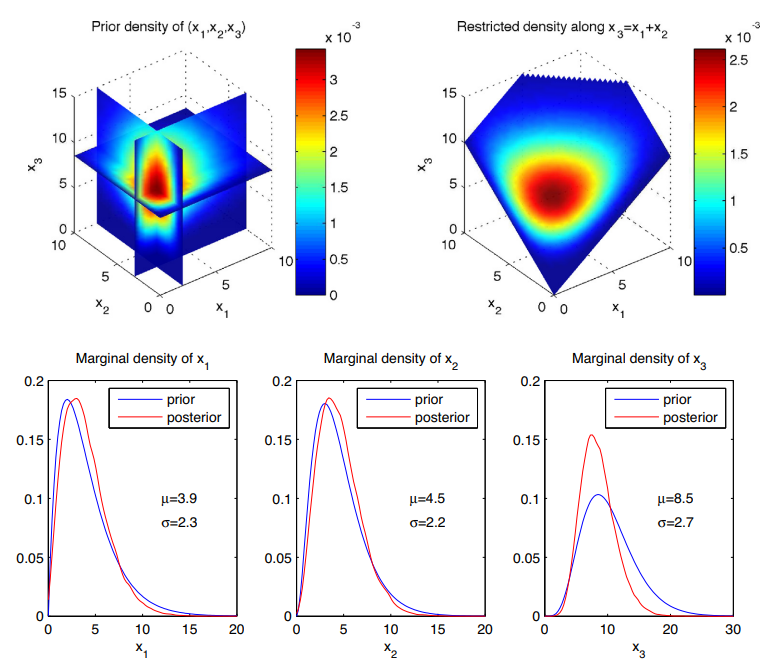
\includegraphics[width=0.5\textwidth]{images/cencic_manifold.png}
\caption{Visualisation of prior distributions with constraint manifold. Top left: prior pdfs of observed variables. Top right: Pdf of variables under constraints. Bottom: Marginalised densities of variables under constraints. Source: \cite{cencic2015general}}
\label{fig:cencic_manifold}
\end{figure}


Cencic et al. derive the posterior distribution of $S$ as:
\begin{equation}
\label{eq:cencic_posterior}
    \pi_s(\bm{w}) = \frac{p_{u}(\bm{h}(\bm{w})) p_{w}(\bm{w}) V(\bm{w})}{\int_W p_{w}(\bm{h}(\bm{w}) p_{u}(\bm{w}) V(\bm{w}) d\bm{w}}
\end{equation}

The term $V(\bm{w}) = \sqrt{|I + H^TH|}$ is a Lebesgue measure of the constraint manifold $S$ where $$H = \begin{bmatrix}
    \frac{\partial h_1{\bm{w}}}{\partial w_1} & \dots & \frac{\partial h_1{\bm{w}}}{\partial w_{n_w}} \\ 
    \vdots & \ddots & \vdots \\
    \frac{\partial h_{n_u}{\bm{w}}}{\partial w_1} & \dots & \frac{\partial h_{n_u}{\bm{w}}}{\partial w_{n_w}} \\
\end{bmatrix}$$ 

$H$ is known as the Jacobian of the dependent variable equations. Cencic et al. argue that the $V(\bm{w})$ term is required to ensure that the posterior distribution being sampled from is invariant no matter which proposal vector $\bm{w}$ is chosen. This is necessary only where the dependent equations are non-linear as with linear equations the Jacobian $H$ does not change for each proposal $\bm{w}$.

% By using a MCMC sampler, the posterior distribution of $S$ can be inferred using proposals of $\bm{w}$. The accepted values for $\bm{w}$ can be used then to calculate the accepted dependent variables.

To avoid computing the denominator of equation \ref{eq:cencic_posterior}, Cencic et al. propose an MCMC sampler known as an independence sampler. For this sampler, the proposal distributions used are the marginal distributions of the free variables, $g(\bm{w}) = p_w(\bm{w})$. The proportional probability of the sampler must be proportional to $\pi_s(\bm{w})$ and therefore is the numerator of equation \ref{eq:cencic_posterior}, $f(\bm{w}) = p_{u}(\bm{h}(\bm{w})) p_{w}(\bm{w}) V(\bm{w})$.

In \cite{cencic2018data}, Cencic et al. evaluate their approach over small MFA models of at most two processes where the functions $\bm{h}(\bm{w}$) are calculated explicitly. Therefore, in generalising it to generic MFA models, a system must be created for selecting which observed variables are to be considered free and which are dependent. Another task is the construction of $n_u$ constraint functions, which incorporate all mass balancing information to express each dependent variable.

\subsubsection{Incremental MFA with Bayesian Inference}
In \cite{lupton2018incremental}, Lupton et al. present an incremental approach to calibrating uncertainty in an MFA model tracking the flow of steel in Austria in 2015. This approach built on the work by Gottschalk et al. by viewing the external inputs $\bm{q}$ and transfer coefficients $A$ as free variables used to calculate the dependent variables; the flows. This approach did not attempt to infer the posterior distribution of a constraint manifold, but rather uses the free variables to calculate dependent prior distributions of the flows, which are then updated by observations. The uncertainty of  the flow value observations were represented as normally distributed random variables. Lupton et al. then updated the dependent observed priors using the likelihood that the observation made came from the dependent observed prior distribution. To construct their model and perform the MCMC sampling, Lupton used a variation of a Hamiltonian Monte Carlo sampler called the No-U-Turn (NUTS) sampler, provided by Pymc3.
% Lupton presents incremental MFA
% Free variables are input * tc in manner of gottschalk, used to create dependent observed variables of flows
% Calibrate parameters with observations of flows
% Uses NUTS sampler which hides away most of the specifics

% TODO check that I either always say variables or parameters

\subsubsection{Hamiltonian Monte Carlo and the No-U-Turn Sampler}
Hamiltonian Monte Carlo (HMC) \cite{betancourt2017conceptual} provides a useful method for sampling a new proposal vector sample from the previous accepted proposal. The Hamiltonian sampler treats the multi-dimensional posterior distribution of model parameters as a concave surface and its log likelihood $\mathcal{L}$ as a negative potential energy function. An accepted proposal parameter $\theta^i \in \bm{\theta}^i$ can be thought of as a coordinate on that surface with $r$ as the momentum of a particle at that coordinate. $L$ "Leapfrog" steps (shown in algorithm \ref{alg:leapfrog}) calculate a new proposal parameter $\theta^{*}$ from $\theta^{i-1}$ by "rolling" this "particle" along the surface with momentum $r$ and distance $\epsilon$ in the direction that maximises the negative energy function. To ensure variation in the next parameter proposed, $r$ is initialised randomly before performing the leapfrogging steps.

\begin{figure}[]
\centering
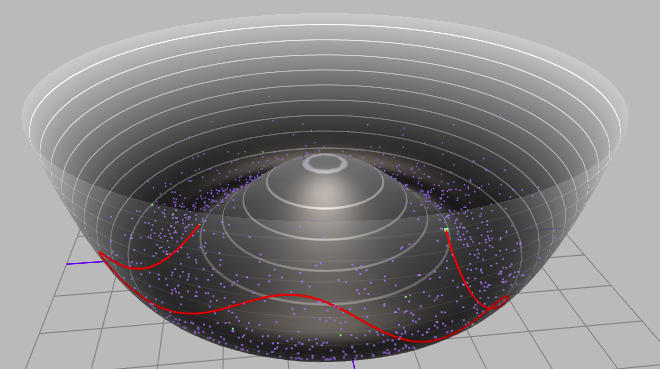
\includegraphics[width=0.5\textwidth]{images/hamiltonian_mcmc.png}
\caption{Visualisation of Hamiltonian Monte Carlo Sampling along a 2-Dimensional posterior probability density function. The red line shows the leapfrog step from the previous accepted proposal value, the green box. Source: \cite{rogozhnikov_2016}}
\label{fig:umis_aspects}
\end{figure}

\begin{algorithm}[h!]
Set $\Tilde{r} = r + (\epsilon/2)\Delta_\theta\mathcal{L}(\theta)$\;
Set $\Tilde{\theta} = \theta + \epsilon \Tilde{r}$\;
Set $\Tilde{r} = r + (\epsilon/2)\Delta_\theta\mathcal{L}(\Tilde{\theta})$\;
\textbf{return} $\Tilde{\theta}, \Tilde{r}$\;
\caption{Leapfrog($\theta, r, \epsilon$)} 
    \label{alg:leapfrog}
\end{algorithm}

$L$ and $\epsilon$ must be tuned correctly during the algorithm to ensure efficient sampling. If $\epsilon$ is too large, the proposal vectors drawn will have been drawn too far away from the previous value and therefore will be rejected too often, wasting computation time. If $L$ is too large, the leapfrogging will perform a "U-Turn" and start moving $\theta$ towards its original value. If $L$ and $\epsilon$ are too small then the proposed values will be too similar to each other and therefore not explore the full space of the posterior distribution. The No-U-Turn sampler (NUTS) \cite{hoffman2014no} automatically tunes $L$ and $\epsilon$ to avoid these issues.

In this thesis, I will adapt the approach by Lupton et al.  to  propagating uncertainty through MFA models for UMIS structured systems. This technique will involve automatically developing a mathematical model from a UMIS diagram with independently observed data values and then using a NUTS sampler provided by Pymc3 to infer the posterior distributions of these values in respect to mass balance constraints. 
% Lupton models the parameters as dependent on the input parameters
\begin{comment}
 - Talk about other approaches for dealing with 
 - Pymc3
  - Lupton
  - Cencic/Stan
  - Cencic offer simplex algorithms as a way for automatically constructing the model but do not implement a program to do so
  - Bayesian Inference
  - A fuzzy set-based approach to data reconciliation in material flow modeling,
        - Can talk about this, can suggest that using probability distributions is better because fuzzy sets have trapezoidal and triangular membership functions which can be modelled as distributions if you use pymc3 correctly
  - we want a general approach to specifying the outputs of the model
  - Probibilistic is flexible to all kinds of uncertainty characterization, intervals can be expressed as uniform, normal, triangular, trapezoidal distributions exist, can show long tail
  - Pymc3 allows specification of their own distributions through interpolated, can construct a triangular or trapezoidal distribution from those
  
  - So its good that you've studied this stuff because you'll want to talk about it in the technical thing
  - First read other technical things and see if they are similar
  - I think for the technical thing the topics are
    - AISHA, read that to see if they indicated a good way to explain the ways that   they built the constraints automatically
    - Fuzzy set theory method 
    - STAN method
    - Mathematical MFA method
    - Sensitivity analysis method
    - Probabilistic MFA, what I use
    - Monte Carlo Markov Chains
    - No-U-Turn, metropolis hastings
    - Pymc3
    
    
\end{comment}



% This chapter is intended to describe the technical basis on which execution
% of the project depends.  The goal is to provide a detailed explanation of
% the specific problem at hand, and existing work that is relevant (e.g., an
% existing algorithm that you use, alternative solutions proposed, supporting
% technologies).  

% Per the same advice in the handbook, note there is a subtly difference from
% this and a full-blown literature review (or survey).  The latter might try
% to capture and organise (e.g., categorise somehow) {\em all} related work,
% potentially offering meta-analysis, whereas here the goal is simple to
% ensure the dissertation is self-contained.  Put another way, after reading 
% this chapter a non-expert reader should have obtained enough background to 
% understand what {\em you} have done (by reading subsequent sections), then 
% accurately assess your work.  You might view an additional goal as giving 
% the reader confidence that you are able to absorb, understand and clearly 
% communicate highly technical material.

% -----------------------------------------------------------------------------

\chapter{Project Execution}
\label{chap:execution}

\section{Overview}
I have developed the following approach for using Bayesian inference to calibrate uncertainty over MFA data structured in UMIS diagrams. The approach is performed in three stages:

\begin{enumerate}
    \item Extract stocks and flows data from STAFDB and arrange in a UMIS diagram
    \item Convert the UMIS diagram into a mathematical model using UMBIE
    \item Display calibrated uncertainty values for stocks and flows data
\end{enumerate}

% The aim for this thesis is to prove UMIS's suitability as a basis for performing computation over industrial ecology systems. To show this I have developed a Bayesian inference engine to propagate uncertainty through UMIS systems and display the calibrated uncertainty values for stocks and flows data. As STAFDB has yet to be publically released, I have developed a prototypical version as a series of CSV files. Information provided by Rupert Myers and Zo\"e Petard from the University of Edinburgh has ensured that the prototype has a similar structure to the version under development. I then extract the stocks and flows data and represent them as a UMIS diagram with Python objects. I then convert the UMIS diagram into a mathematical model and infer calibrated uncertainty values as histograms for the stocks and flows data using MCMC sampling. Calibrated uncertainty values can then be estimated from the histogram data.

\section{Constructing the UMIS Diagram}

\subsection{STAFDB Prototype}
\label{sec:prototype_stafdb}
As STAFDB has not yet been released, I have developed a prototypical version (STAFDB-P) for my implementation. This database was constructed as CSV files and accessed via \texttt{Pandas} operations. I was provided an Entity Relationship Diagram (ERD) for in-progress STAFDB by Zo\"e Petard from the University of Edinburgh. This can be seen in appendix \ref{appx:stafdb_erd}. As only a subset of the entities in the database are necessary for the inference engine, the STAFDB-P only contains that subset. An ERD describing the prototype can be seen in figure \ref{fig:prototype_ern}.

\begin{figure}
    \centering
    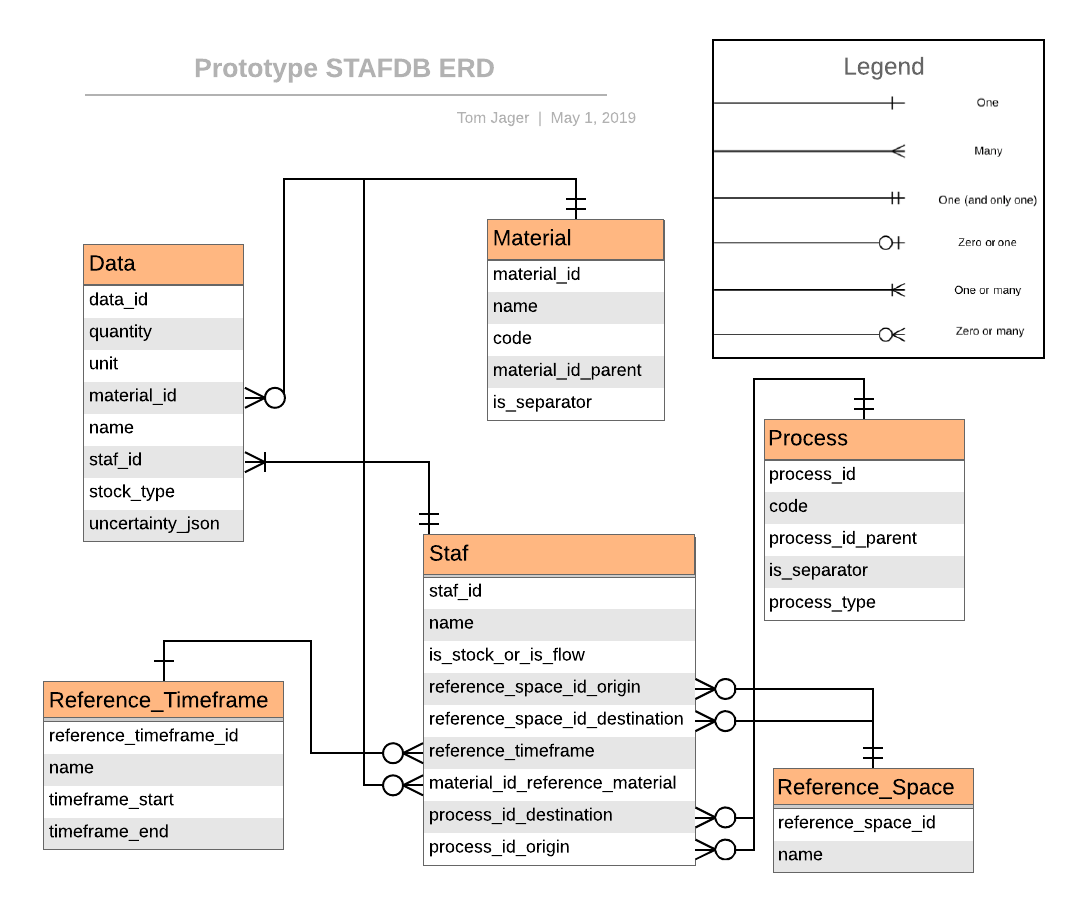
\includegraphics[width=\linewidth]{images/Prototype_STAFDB_ERD.png}
    \caption{Entity Relationship Diagram showing the schema of STAFDB-P}
    \label{fig:prototype_ern}
\end{figure}

STAFDB is designed around describing all industrial ecology systems in terms of stocks and flows. These are consolidated into a single entity, staf. Each staf has associated descriptive attributes for the space, primary material, time-frame and processes they are in reference to. The staf is also associated with at least one data value containing information regarding the quantity, unit and specific material that is flowing or being stored. Stafs are associated with multiple data values when they are describing a composite material with multiple fundamental components. Each data value describes a fundamental component of the composite material. STAFDB also stores information regarding the provenance of the data, such as the data's quality and the study it has originated from. In \cite{laner2014systematic}, Laner describes a method for expressing a data's quality as uncertainty in the form of normal and log-normal distributions, however no definitive uncertainty characterisation method has been proposed yet for STAFDB. Therefore I have replaced information regarding the provenance of the data with JSON strings describing the data's uncertainty. The uncertainty can be characterised as uniform with a lower or upper bound, or as normally or log-normally distributed with a mean and standard deviation.

\subsection{UMIS Diagram}
% A UMIS diagram is constructed from three components, a list of external flows entering the system, a list of stocks and flows internal to the system, and a list of flows exiting the system.
\label{sec:python_umis_diagram}
A UMIS diagram is used to represent the relationship between stocks, flows and processes in a single system. STAF records are first extracted by their ID from STAFDB-P and parsed into sets of \texttt{Stock} and \texttt{Flow} Python objects as well as their related attributes. Stocks and flows are separated from STAFs in a UMIS diagram as they have differing behaviour.

Both \texttt{Stocks} and \texttt{Flows} inherit from a \texttt{Staf} class which has attributes for time-frame, material, origin process and destination process. \texttt{Stock} and \texttt{Flow} also have a dictionary which maps a fundamental material to its \texttt{StockValue} and \texttt{Value} respectively. These values are the information regarding the quantity of that material being stored or flowing. Both \texttt{StockValue} and \texttt{Value} store the quantity, unit and uncertainty around the data where the uncertainty is the serialised JSON string described in section \ref{sec:prototype_stafdb}. The uncertainty classes and their attributes can be found in figure \ref{fig:UmisDiagram}. \texttt{StockValue} contains an additional field describing the "stock type" which is either "Net" or "Total". This is because stocks in STAFDB may refer to the total amount stored at that process or instead the net transfer of material to or from storage during this time-frame. This approach will focus on static MFA and therefore looks only at the movement of material during a single time-frame. Therefore whilst total stock values are accommodated by the UMIS Python objects they are ignored when constructing the model.

Origin and destination processes for stocks and flows are parsed into \texttt{UmisProcess} objects. In STAFDB, processes are generalised so that one process record can be used to describe the same event in various locations. For example a manufacturing process in STAFDB can be used to represent manufacturing in Spain or the UK. In a UMIS diagram, processes must be differentiated by location (space) as flows between the same processes but in different reference spaces are supported. Therefore \texttt{UmisProcess}'s have a unique diagram ID formed of concatenating their process ID and their reference space ID. Processes also store information about their type and name. When a flow is parsed, its origin and destination process is validated to ensure that they are between a transformation and distribution process. Likewise, stocks are validated to ensure that they are between a storage and a transformation or distribution process.

UMIS diagrams are implemented as the class \texttt{UmisDiagram}. They are constructed from sets of external flows entering the diagram, internal stocks and flows in the diagram, and flows exiting the diagram. In agreement with the findings of Myers and Pauliuk \cite{myers2019unified, pauliuk2015general}, the diagram follows a graph pattern \cite{klein}. Therefore, external inflows and external outflows to the system are stored as separate sets, whilst the internal flows and stocks in the diagram are stored as a dictionary mapping each internal process to its outflows and its stock if it has one. Consequently the system structure is stored as the External Inflows, the External Outflows and the Process Stafs Dictionary. The intention is to develop a Pythonic representation of a UMIS diagram that is decoupled both from STAFDB and from the Bayesian inference engine. Therefore if further computational models or visualisation tools are developed, they can build directly off of the Python classes, without having to write new methods for extracting the data from STAFDB. A UML diagram of the structure of \texttt{UmisDiagram} and its components can be seen in figure \ref{fig:UmisDiagram}.

\begin{figure}
    \centering
    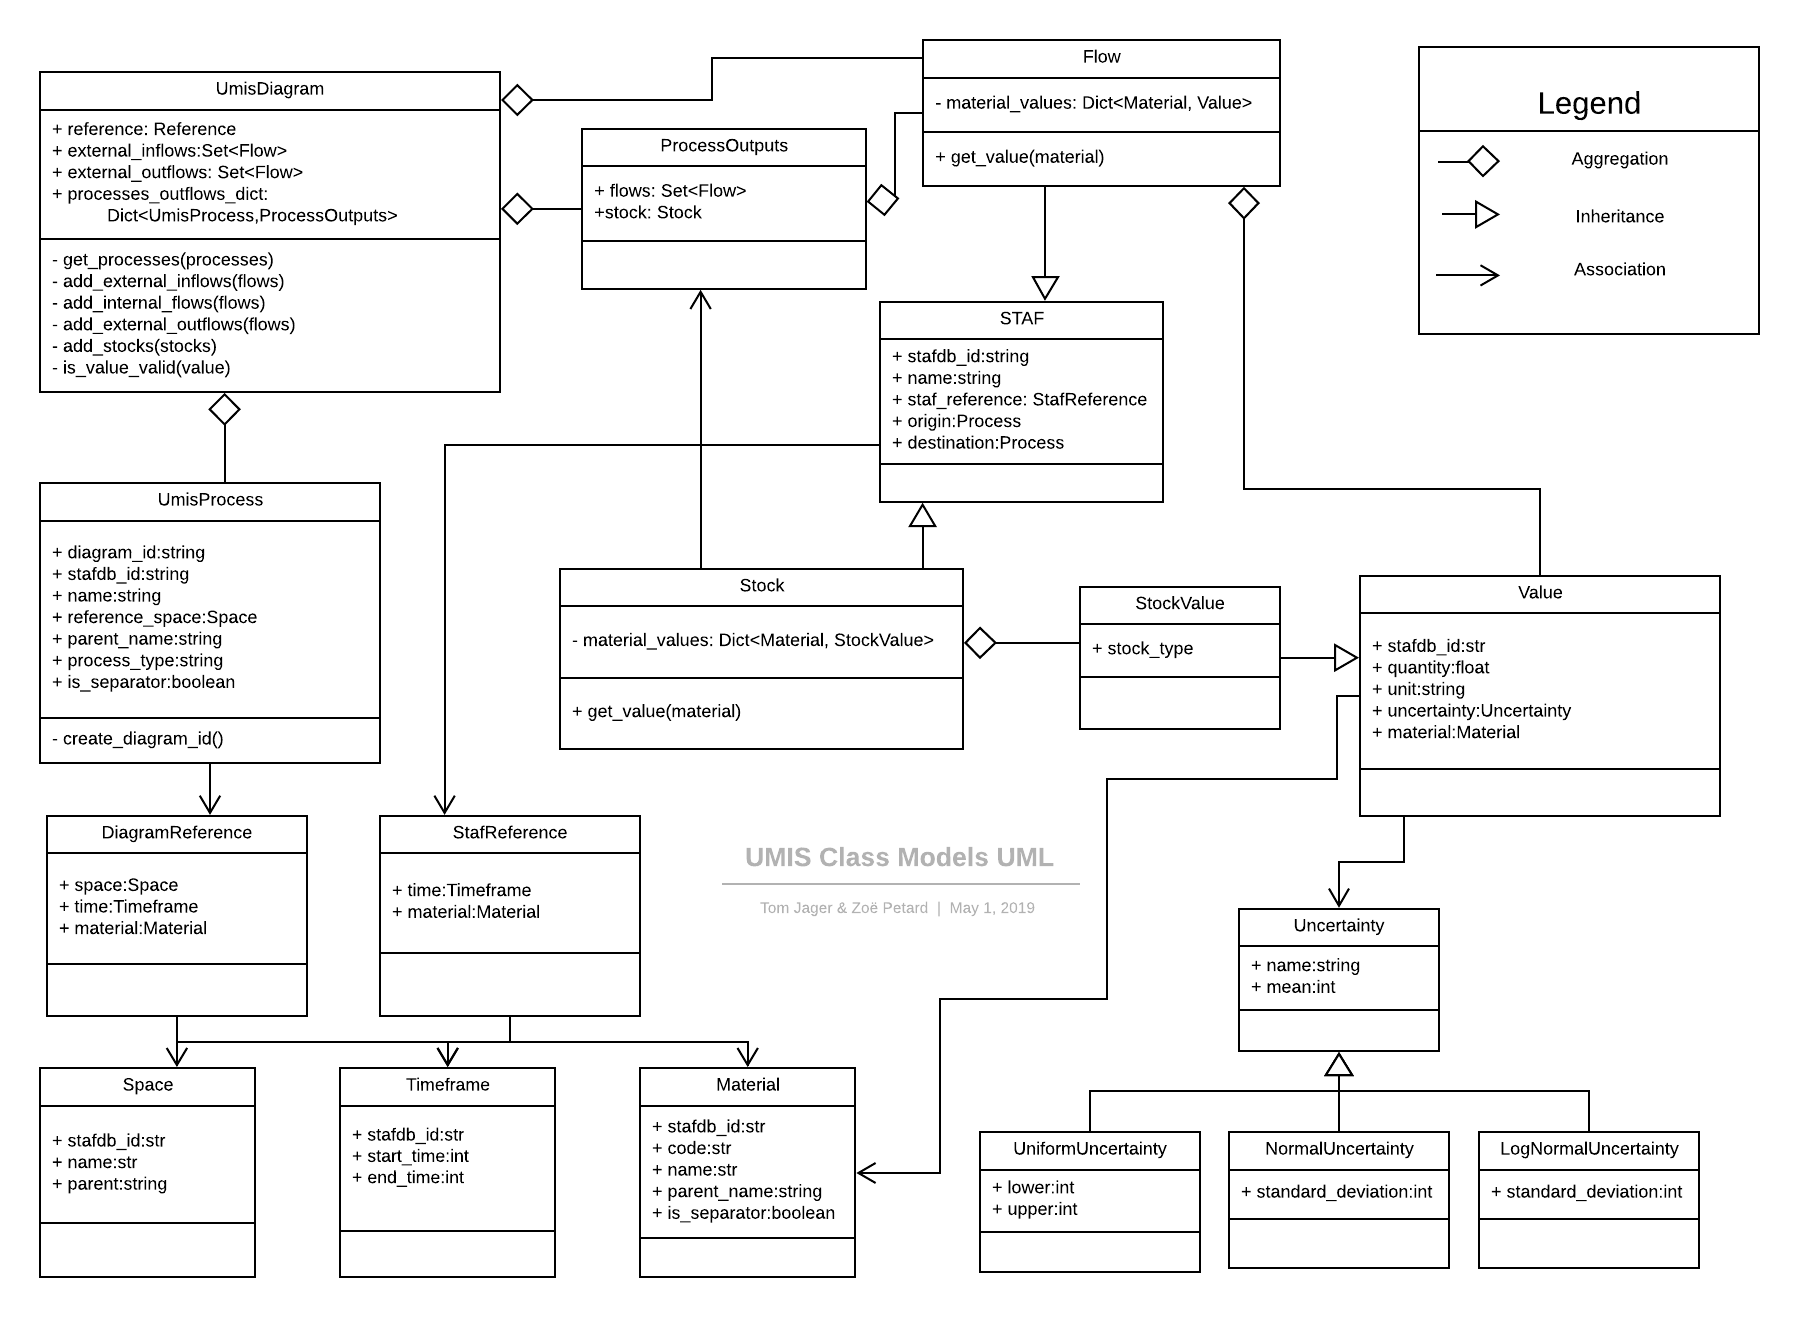
\includegraphics[width=\textwidth]{images/UMIS-data-models.png}
    \caption{UML Class diagram of UMIS diagram data models}
    \label{fig:UmisDiagram}
\end{figure}

Once stocks and flows have been organised into a UMIS diagram, a Bayesian inference approach can be used to infer their calibrated uncertainty values in respect to the system.

\section{Constructing the Mathematical Model}
\subsection{A System of Equations}
In \cite{gottschalk2010probabilistic}, Gottschalk et al. use equation \ref{eq:gottschalk_eq} to represent the mass balance constraints of the system. Lupton et al. extends this using equation \ref{eq:mass_balance_3}  to develop an equation for system flows:
% where $I$ is the identity matrix, $A$ is a matrix of transfer coefficients (TCs) and $a_{ij} \in A$ is the TC from equation \ref{eq:mass_balance_3}, representing the proportion of throughput from process $i$ that moves to process $j$. $\bm{z}$ is a vector of process throughputs as mentioned in equation \ref{eq:mass_balance_2}, $\bm{q}$ is a vector of external inflows to each process from outside the system, and $\bullet$ is the dot product operation.

\begin{equation}
    F=A \cdot \bm{z}
\end{equation}

where $f_{ij} \in F$ is the flow from process $i$ to process $j$ and $\cdot$ is the elementwise multiplication operation. Therefore equations for each outflow from processes in Gottschalk's models can be derived as:

\begin{equation}
    F=A \cdot (I-A^T)^{-1} \bullet \bm{q}
\end{equation}

% with a known prior distribution ($p(A)$, $p(\bm{q})$). This prior distribution does not need to be specific, for example the knowledge that all TCs must be between 0 and 1 and that the sum of all outgoing TCs for a process must equal 1 is often sufficient and can be applied to all TCs.
% There is a known prior distribution of these values ($(p(F)$) which is independent from the prior distribution of the free parameters. These prior distributions can take the form of 

Whilst this equation was sufficient for Lupton and Gottschalk's case studies, UMIS systems can include the use of stocks where material flow in and out of a virtual reservoir, therefore this concept must be accommodated. To do this stock values are separated into two types. In the first, material is stored into the virtual reservoir ($\bm{s^-})$. These are now treated as an extra outflow from an existing process into a new storage process. As such they have their own TCs ($A'$) and staf equations ($F' = \begin{bmatrix}
F & \bm{s^-}
\end{bmatrix}$). In the second type, material enters the system from the virtual reservoir ($\bm{s^+}$); these are now treated as another form of inputs to processes in the system ($Q = \begin{bmatrix}\bm{q} & \bm{s^+}
\end{bmatrix}
$).

Another adaptation is to allow for the storage and flow of composite materials. For this, concentration coefficients (as in equation \ref{eq:mass_balance_4}) must be included in order to reconcile the flow of composite materials into a reference material. In order to ensure that the system of equations is mass balancing correctly and that the likelihoods of dependent parameters are being calculated in terms of the same material, concentration coefficients are needed to reconcile staf values for composite materials into the reference material. Input parameters ($Q$) are converted into the reference material through:

\begin{equation}
    Q_r = Q \cdot {C_{Q}}
\end{equation}

The results from staf equations must also be converted from the reference material into the material that is observed through:
\begin{equation}
    F'_o = \frac{F'}{C_{F'}}
\end{equation}


Therefore the system of equations for my model is:

\begin{equation}
    F'_o = \frac{A' \cdot (I-A'^T)^{-1} \bullet sum(Q \cdot C_Q)}{C_{F'}}
    \label{eq:my_model_eq}
\end{equation}

% In the context of Cencic's framework, $A$ and $\bm{q}$ can be seen as free observed parameters and matrix $F$ can be seen as a matrix of dependent observed parameters constructed from free parameters. 
To put this in the context of Cencic's framework discussed in section \ref{sec:bayesian_inference}, matrices $A', Q, C_Q$ and $C_{F'}$ are the free variables ($\bm{w}$), $F'_o$ is a matrix of dependent stock and flow variables ($\bm{u}$) and equation \ref{eq:my_model_eq} is the function mapping the free variables to the dependent values ($\bm{h}(\bm{w})$). 

% To implement Cencic's framework and sample from the posterior distribution of the constrained model parameters, the sampler must be able to draw from the correct proposal distribution and calculate the correct acceptance probability equivalent to that of the calibrated posterior distribution. As each model parameter is assumed to be independent, the proposal vector of the free variables is drawn from their own prior distributions. 

% NOTE to derive the proportional thing it needs the likelihood, the probability of drawing vector p and this jacobian term. 

\subsection{Characterising Stocks, Flows and Concentration Coefficients}
\label{sec:characterising_stocks_and_flows_and_ccs}
Each parameter in the model has a known prior distribution which characterises the uncertainty around that parameter's true value. For $Q$, $F'_o$, $C_{Q}$ and $C_{F'}$ these are represented as normally, log-normally or uniformly distributed stochastic variables whose distribution parameters are $\{\mu_n, \sigma_n\}$, $\{\mu_l, \sigma_l\}$ and $\{l_u, u_u\}$ respectively. In cases where the parameter value is unknown, this can be modelled by an uninformative, wide uniform distribution. The prior distributions for $F'_o$ and $Q$ are supplied when constructing the UMIS diagram and take the form of \texttt{Uncertainty} attributes in the corresponding \texttt{StockValue} and \texttt{Value} objects. A material reconciliation table is supplied to the system and is used to map materials to the prior distributions of CCs. In cases where the CC of a material is a known constant, it is represented by a \texttt{Constant} Python object. 

\subsection{Characterising Transfer Coefficients}
\label{sec:representing_tcs}
TCs have a more interesting prior distribution as it is dependant on the structure of the model and differs according to their origin process type. Lupton et al. also recognise the division of transformation and distribution processes and propose characterising the TCs of each process type through different distributions. For both types, if a process only has one outflow then its TC must be 1, whilst if there are no outflows, the TC must be 0. In some cases, the modeller may have prior knowledge of TC values that they wish to supply to the model. This can be done through the use of a TC look-up table which maps the origin and destination process IDs of the TC to an \texttt{Uncertainty} object. 

Transformation processes can have at most two outflows: a stock and an outflow to another process. In this case, the TCs are $\theta$ and $1-\theta$. If no prior knowledge of the TC exists, then $\theta$ is represented as a uniform distribution between 0 and 1. If prior knowledge about one TC exists in the look-up table, $\theta$ is represented as the stochastic variable from that \texttt{Uncertainty}. If prior knowledge about both exists, then one is arbitrarily selected to represent $\theta$.

Distribution processes can have many outflows, including to stock. Lupton models these TCs as parameters from a Dirichlet distribution. A Dirichlet distribution is a continuous multivariate distribution with two parameters $\bm{\alpha}$ and $\bm{\theta}$ \cite{dirichlet}. Drawing from a Dirichlet distribution results in $\{\theta_1, ..., \theta_n\} = \bm{\theta}$ where $\sum_{i}\theta_i = 1$ and $\theta_i \ge 0$. This makes it ideal for representing TCs which share the same properties. The share parameters $\{\alpha_1, ..., \alpha_n\} = \bm{\alpha}$ indicate a weighting to a certain configuration of $\bm{\theta}$. Figure \ref{fig:dirichlet} shows the effect of $\bm{\alpha}$ on a three parameter Dirichlet distribution. If no prior knowledge of TCs exist, each $\alpha_i$ is set to 1 resulting in every possible configuration of TCs being equally likely. If prior knowledge of any TC exists in the look-up table, its $\alpha$ is set to the mean of the \texttt{Uncertainty} object.

\begin{figure}
    \centering
    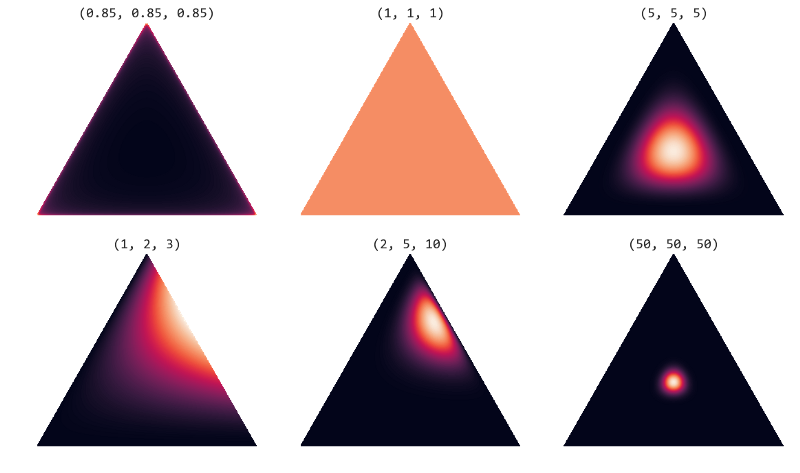
\includegraphics[width=0.75\textwidth]{images/dirichlet.png}
    \caption{Effect of $\bm{\alpha}$ on a three parameter Dirichlet distribution. Source: \cite{dirichlet}}
    \label{fig:dirichlet}
\end{figure}

\subsection{Model Construction}
\label{sec:model_construction}
To construct our model, we will follow the method of Lupton et al. by using Pymc3 and Theano to create model parameters and define the dependent equations. Pymc3 allows for the construction of mathematical models through stochastic, observed stochastic and deterministic random variables. The stochastic random variables represent the free variables $\bm{w}$ in the model. Deterministic random variables represent the result of transformations applied to values drawn from random variables. During sampling the deterministic values are calculated from accepted proposals of the free variables and stored. They are used to represent the dependent variables $\bm{u}$. Observed stochastic random variables are used to represent likelihood terms in a model. In this approach, they incorporate the probability of observing a calculated dependent parameter given the prior distribution of that parameter $p_u(\bm{h}(\bm{w}))$. Pymc3 comes built in with observed stochastic and stochastic random variables representing uniform, normal and log-normally distributions.

% create his mathematical model from stochastic variables, observe the likelihood of his dependent parameters and sample from the resultant posterior distribution. He used Theano operations to define the equations in his system. We will use the same tools in our approach. Construction of the model before sampling can be split into three steps:  

Construction of a Pymc3 model from a UMIS diagram is performed in three steps: Defining the parameter priors, creating the model parameters and equations, and observing the dependent parameters to calculate their likelihood. This structure is illustrated in figure \ref{fig:inference_engine_structure}. These steps are performed when constructing a \texttt{UmisMathModel} instance. It takes the following inputs:

\begin{table}[h!]
\begin{tabular}{|p{6cm}|p{9cm}|}
\hline
\textbf{Input Parameter}               & \textbf{Description}                                                                                                                      \\ \hline
External Inflows                       & Set of flows that are external inflows to processes in the UMIS diagram                                                                   \\ \hline
Process Stafs Dictionary               & Dictionary mapping internal processes to their outflows and stocks                                                                        \\ \hline
External Outflows                      & Set of flows that are external outflows from processes in the UMIS diagram                                                                \\ \hline
Reference Material                     & Specific material over which the system is mass balanced                                                                                  \\ \hline
Reference Time-Frame                   & Specific time-frame over which the system is mass balanced                                                                                \\ \hline
Material Reconciliation Table          & Dictionary mapping a composite material to an Uncertainty \mbox{object} representing its concentration coefficient                               \\ \hline
Transfer Coefficient Observation Table & Dictionary storing prior information about transfer \mbox{coefficient} \mbox{values}. Its design and use is discussed in \mbox{section} \ref{sec:representing_tcs} \\ \hline
\end{tabular}
\caption{Inputs to the \texttt{UmisMathModel} instance}
\label{tab:math_model_inputs}
\end{table}

The reference attributes refer to the specific time-frame and material over which the system is mass balanced. When processing stocks and flows, those belonging to the wrong time-frame are ignored, whilst those with no value for the reference material undergo material reconciliation. 

Material reconciliation allows for the use of concentration coefficients in the MFA model. It checks to see if the stock or flow has any value for a material corresponding to an entry in the material reconciliation table. If so, that value is used and that material's CC is stored for use later. If a stock or flow has no material that can be reconciled, it is ignored. If material reconciliation is not necessary, a \texttt{Constant} CC of 1 is used.


% \newgeometry{left=0cm,bottom=0cm, right=0cm,top=0cm}
\newgeometry{right=2cm,bottom=2cm, top=2cm, left=2cm}
\begin{figure}
    \centering
    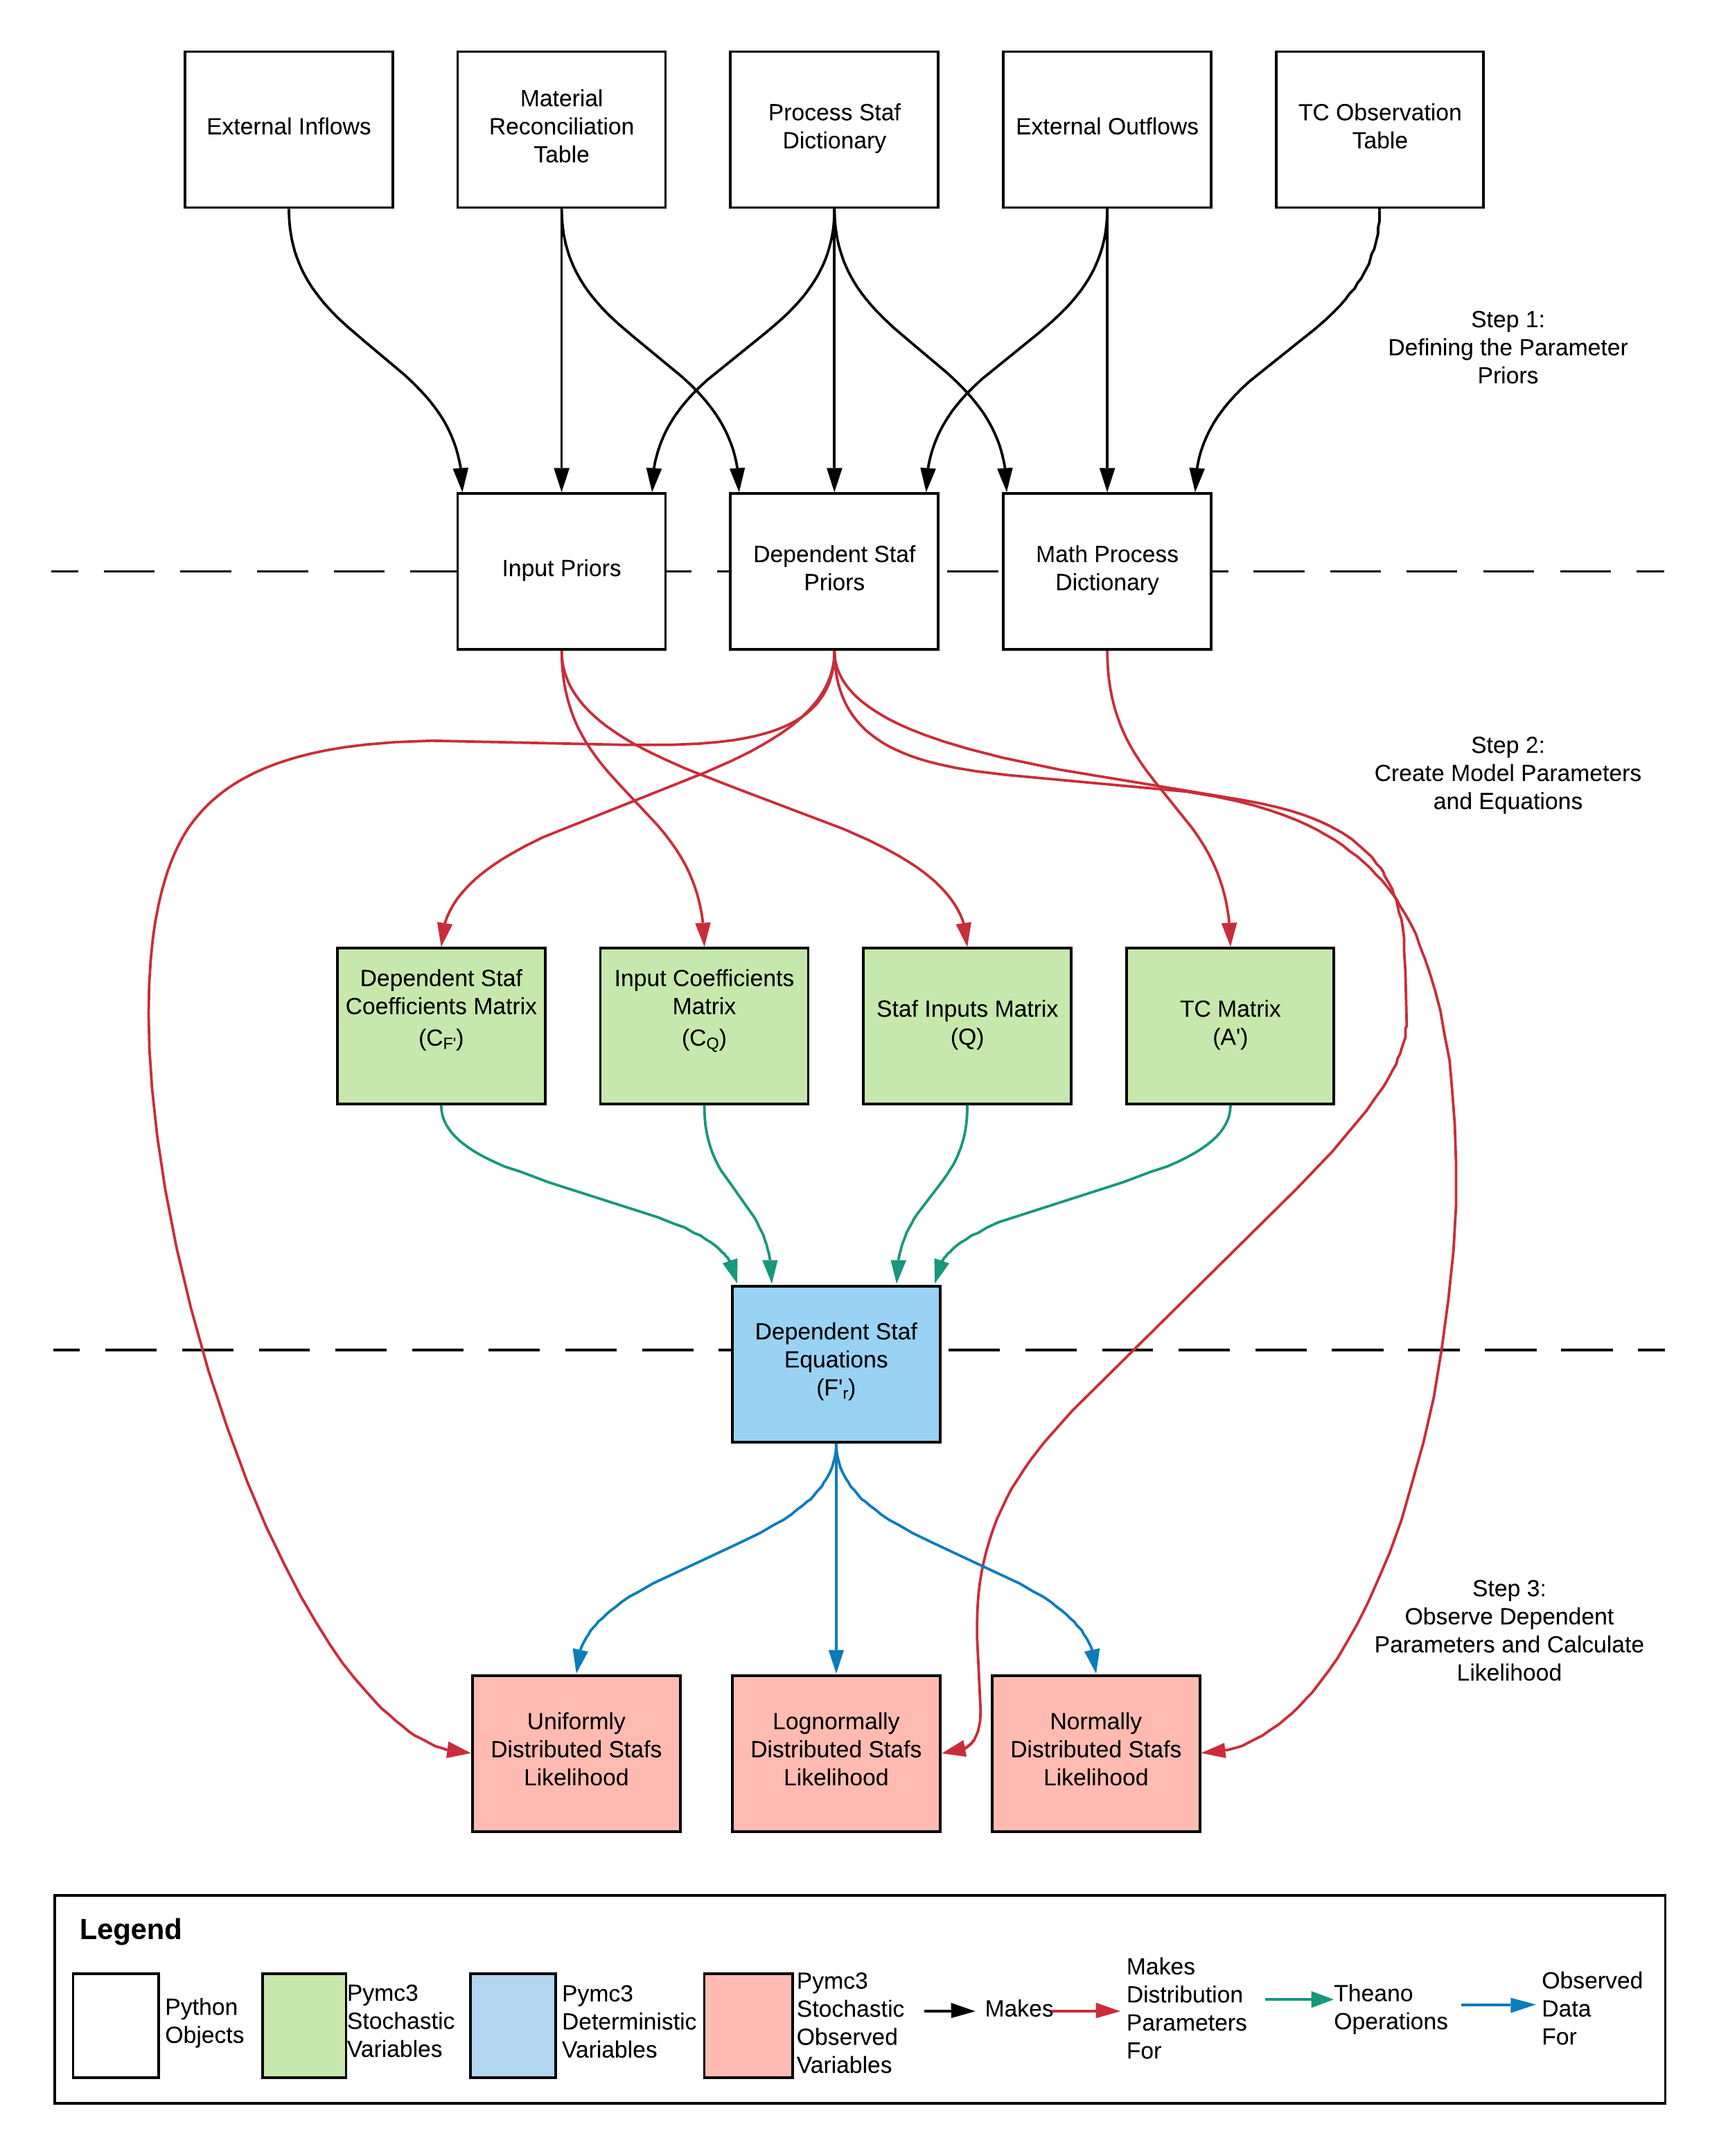
\includegraphics[width=\linewidth]{images/inference_engine_structure.png}
    % 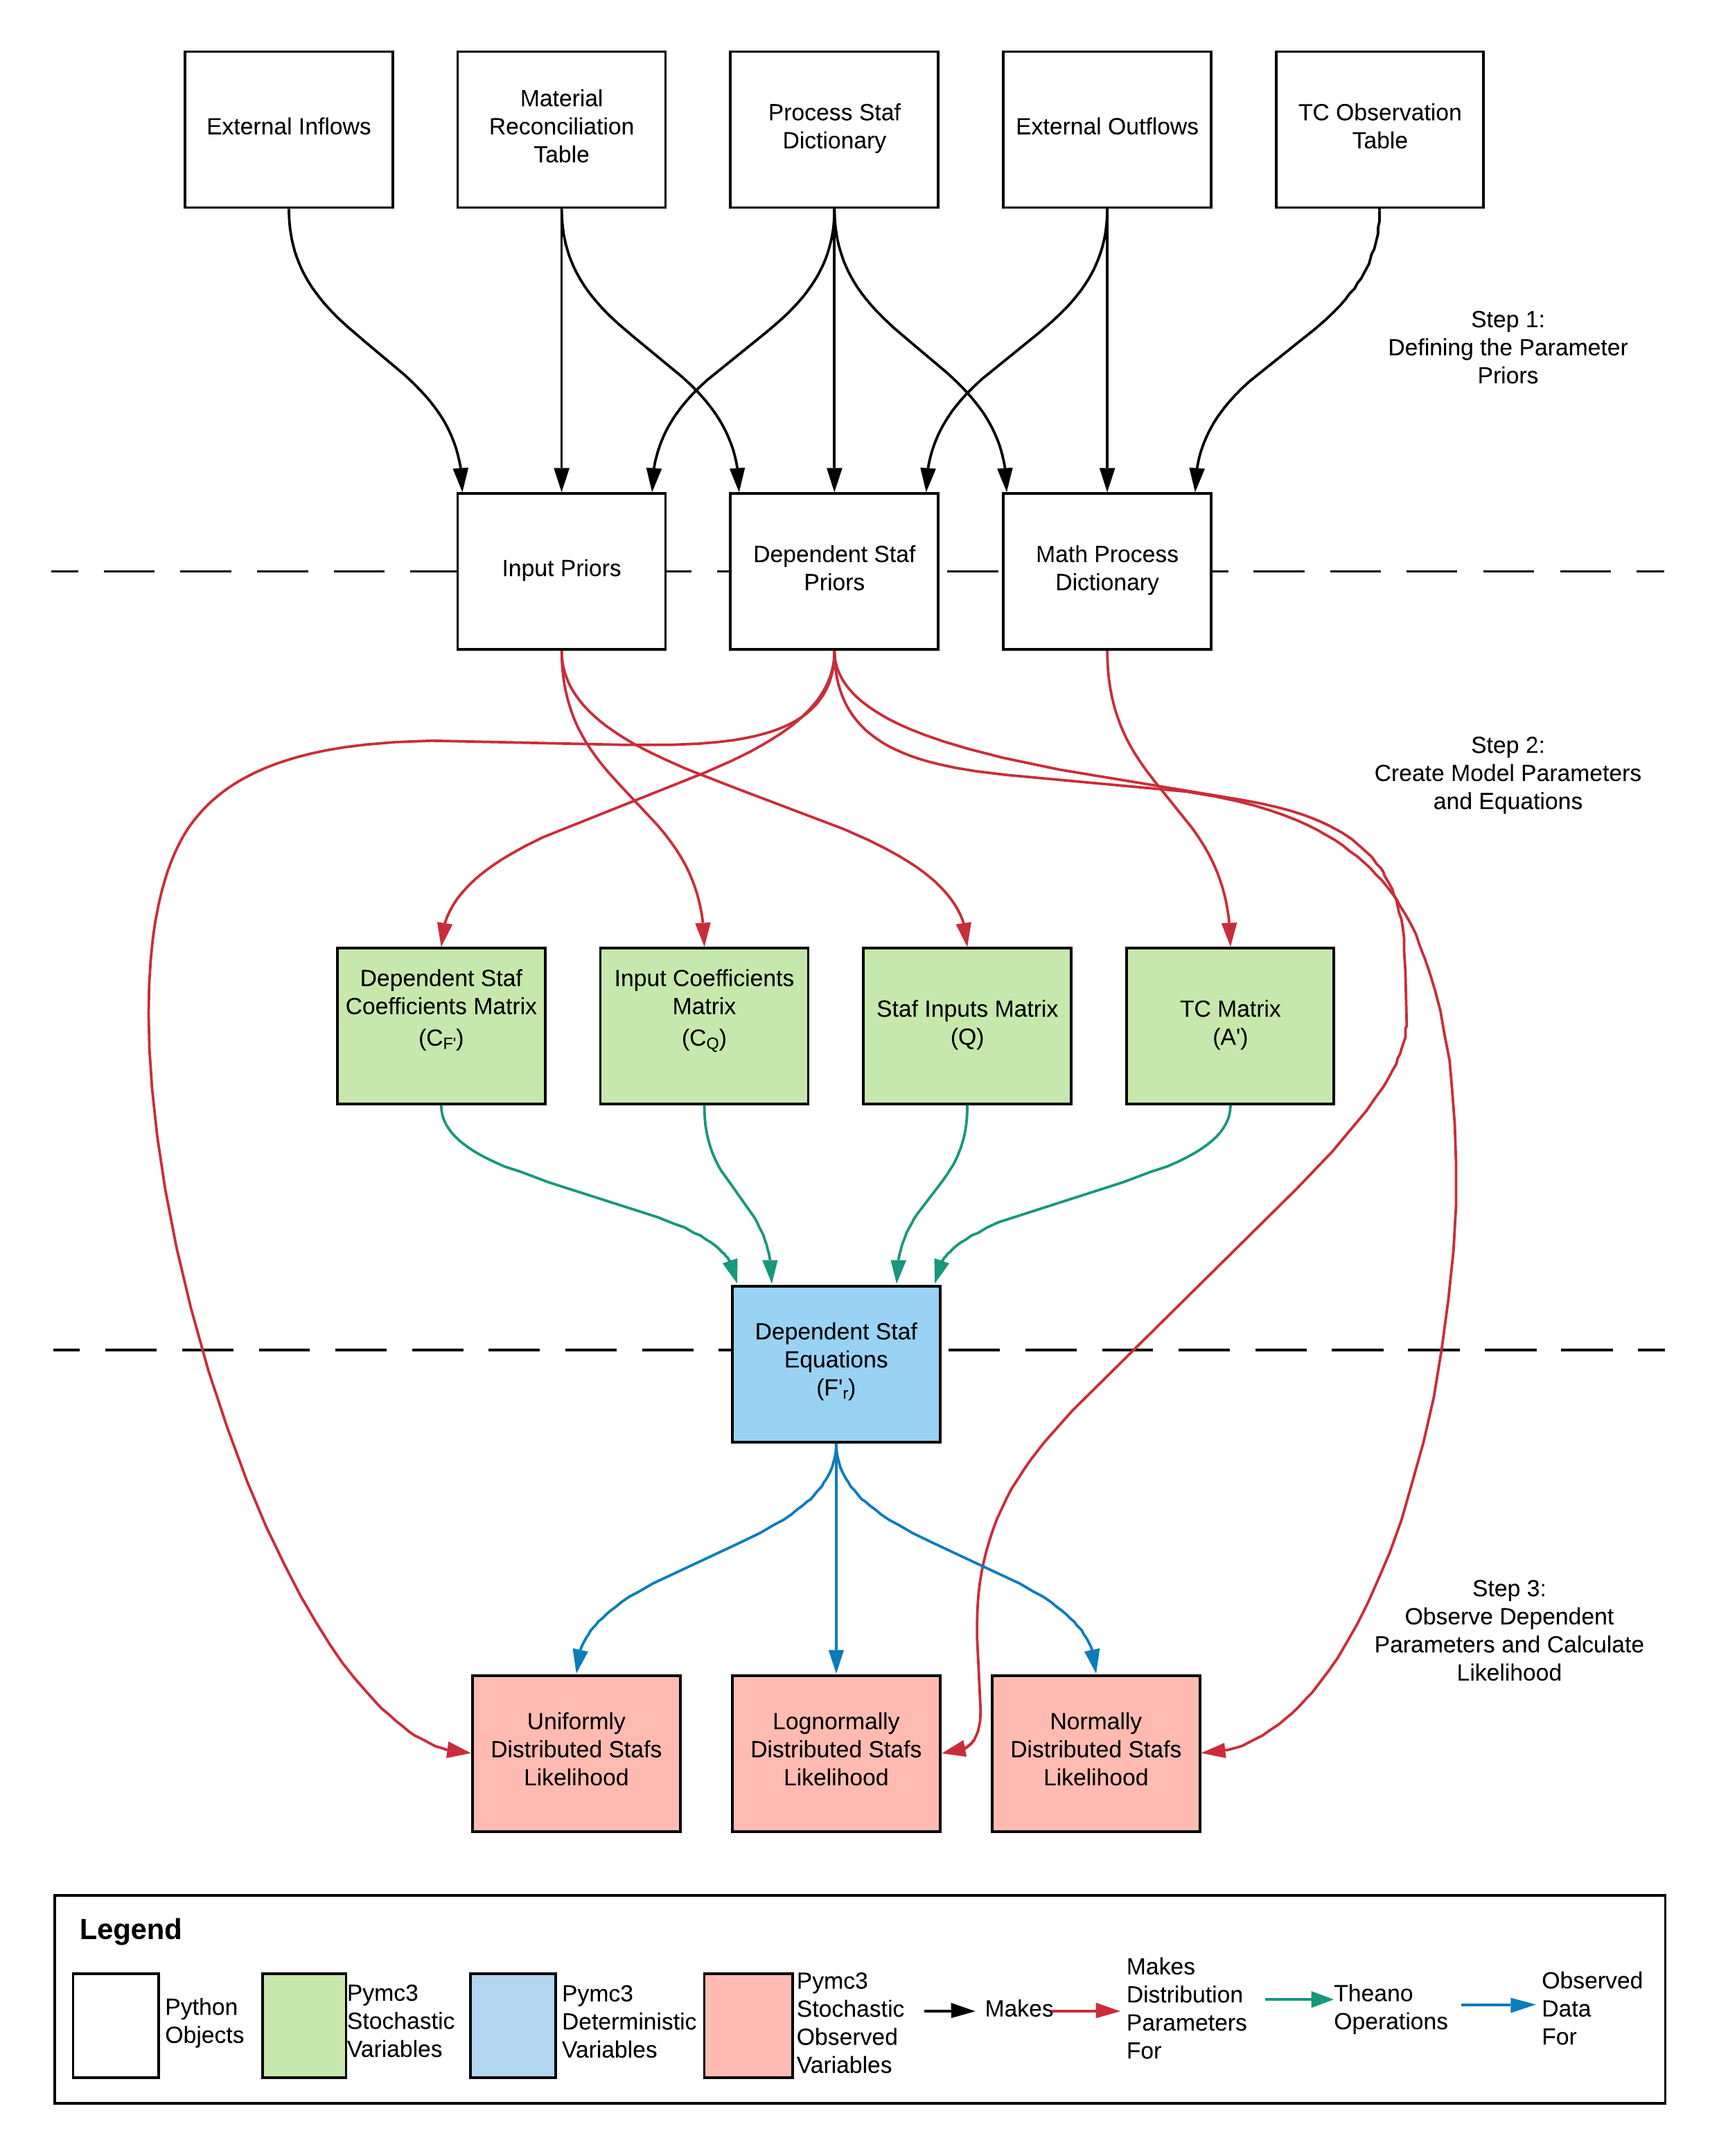
\includegraphics{images/inference_engine_structure.png}
    \caption{Structure of model construction for the Bayesian inference engine}
    \label{fig:inference_engine_structure}
\end{figure}
\restoregeometry

\subsubsection{Step 1: Defining Parameter Priors}


The first step is devoted to creating Python objects responsible for creating the stochastic random variables in the model. All model parameters are stored as ParamPrior objects These contain a parameter's type (e.g TC), origin process ID, destination process ID and an \texttt{Uncertainty} attribute which describes the parameter's prior distribution. These objects have a method to create a Pymc3 stochastic variable corresponding to the parameter's \texttt{Uncertainty}.

First the Math Processes are created which are accessed through the Math Process Dictionary. This maps the diagram ID of the process to its corresponding Math Process. On creation of a new Math Process it is assigned an incremental process index which refers to its row in the parameter matrices. The dictionary provides a way for finding the matrix index of a process from its diagram ID. Construction is performed by iterating over the Internal Stafs Dictionary and External Outflows.

Outflows are added to a process as ParamPrior objects. For these ParamPrior objects, the \texttt{Uncertainty} refers to the prior knowledge of the outflow's TC. A Math Process's outflows are used to create a list of process IDs that receive flows from it, and a corresponding list of stochastic variables representing its TCs. These stochastic variables are constructed in accordance with section \ref{sec:representing_tcs}. Stocks going to the virtual reservoir ($s^-$) are represented as an outflow to new process, whilst stocks that are coming from the virtual reservoir ($s^+$) are ignored.

Next the InputPriors object is created. This contains two dictionaries, one mapping process IDs to their inputs from external inflows (External Inflows Dictionary) and the other mapping process IDs to the inputs from the virtual reservoir (Stock Inputs Dictionary). Each input is represented by two ParamPrior objects, one representing the unreconciled staf value flowing into the system ($\{q_i | s^+_i\} \in Q$) and the other representing its CC ($c_Q \in C_Q)$. The External Inflows Dictionary are construct from the External Inflows set and the Stock Inputs Dictionary is constructed from the Internal Stafs Dictionary.

The final Python object is the Dependent Staf Priors. This is a list of Dependent Staf Prior objects. Each Dependent Staf Prior consists of two ParamPrior objects, one representing the un-reconciled observed distributions of the dependent model parameters ($f'_o \in F'_o$) and the other representing its CC ($c_r \in C_{F'}$). Dependent Staf Priors separate the observed parameters into three lists by their distributions.

\subsubsection{Step 2: Create Model Parameters and Equations}
Once the Python objects have been created they are used to develop a Pymc3 mathematical model. The matrices in the right hand side of equation \ref{eq:my_model_eq} are constructed as Theano tensors and then populated either by Pymc3 stochastic variables or constants.

First the TC matrix ($A'$) is constructed from the Math Process Dictionary. It is initialised as an $N_p \times N_p$ dimensional Theano tensor matrix of zeros, where $N_p$ is the number of processes in the system (including new ones created from stock values). The Math Process Dictionary is then used to create the Pymc3 stochastic random variables for each TC and place them in the correct positions in the matrix. The CC matrix for staf values is created in a similar manner but is initialised with ones.

The Staf Inputs Matrix ($Q$) and its corresponding Input Coefficients Matrix ($C_Q$) are initialised as $N_p \times 2$ Theano tensor matrices of zeros and ones respectively, with one column referring to the external inflows ($\bm{q}$) and the other referring to the stock arriving from the virtual reservoir ($\bm{s^+}$). These matrices are populated by stochastic random variables from the Input Priors. By adding these random variables to the Pymc3 model they are set as free variables in a mathematical model. Later when this model is sampled from, proposals will be drawn as a vector of these free variables. Theano operations are then used to implement equation \ref{eq:my_model_eq} resulting in a Theano matrix representation of $F'_o$.

Each Theano matrix as a whole is set as a named Pymc3 deterministic variable. When this model is sampled, Pymc3 will then store the value of each matrix for each sample. This allows us to extract the posterior samples of each matrix from their variable name and then access the samples of specific parameters using their location in that matrix.

\subsubsection{Step 3: Observe Dependent Parameters to Calculate Their Likelihood}
Construction of the model is finished by incorporating the likelihood of observing $F'_o$, given their known prior distributions. The Dependent Staf Priors object is used to create an observation matrix for each type of distribution $d$. An observation matrix $\Omega$ is an ${N_k \times N_p \times N_p}$ matrix, where $N_k$ is the number of stafs observed to have that particular distribution. It is constructed through algorithm \ref{alg:observation_matrix}:

\begin{algorithm}[h!]
    $N_k =$ Number of stafs observed to be distributed as $d$\;
    $N_p =$ Number of processes in model\;
    $\Omega = (0)^{N_k \times N_p \times N_p}$\;
    \For{$k = 1$ to $N_k$}{
        $e_k$ = $k_{th}$ staf observation distributed as $d$\;
        $i$ = $e_k$ origin process index\;
        $j$ = $e_k$ destination process index\;
        $\Omega[k,i,j] = 1$\;
    }
    \caption{CreateObservationMatrix($d$)}
    \label{alg:observation_matrix}
\end{algorithm}


% Each observation $k$ of staf $f'_{ij} \in F'_o$ results in $\omega_{kij} = 1, \omega_{kij} \in \Omega$ for that distribution's observation matrix. The rest of the cells are 0.

$\Omega \circ F'_o$ (where $\circ$ is the Theano \texttt{tensordot} operation) then results in an $N_k \times 1$ vector of the staf equations $f'_{ij}$ which have been observed to have the particular distribution of $\Omega$.

The observation matrices are used to extract the values of $F'_o$ which are normally, log-normally and uniformly distributed ($\bm{f'_n}, \bm{f'_l}, \bm{f'_u}$). The Dependent Staf Priors object also produces distribution parameter vectors $\{\bm{\mu_n}, \bm{\sigma_n}\}$, $\{\bm{\mu_l}, \bm{\sigma_l}\}$ and $\{\bm{l_u}, \bm{u_u}\}$. The likelihood of the dependent vectors are then added to the model through Pymc3 observed stochastic variables as: 
$$ p(\bm{f'_n} | Normal(\bm{\mu_n}, \bm{\sigma_n^2})),$$
$$p(\bm{f'_l} | Lognormal(\bm{\mu_l}, \bm{\sigma_l^2})),$$
$$p(\bm{f'_u} | Uniform(\bm{l_u}, \bm{u_u})) $$

This differs from the approach of Lupton et al. where the likelihoods are created as $p(\bm{\mu_n} | Normal(\bm{f'_n}, \bm{\sigma_n^2}))$. Their approach treats the priors of the staf values as the result of calculations from the free parameters and then updates those priors with the observations of staf values. Instead we have used Equation \ref{eq:cencic_posterior} derived by Cencic et al. \cite{cencic2018data}, which suggests using the likelihood of observing each calculated value from their known prior distribution. This allows us to use this approach for log-normal and uniform likelihoods.

\section{Displaying Calibrated Uncertainty Data}
The UMIS diagram has been converted into a Pymc3 mathematical model containing the following terms:

\begin{itemize}
    \item Free Priors - $p(A'), p(Q), p(C_Q), p(C_F')$
    \item Deterministic Variables - $F'_o$
    \item Observed Likelihood - $ p(\bm{f'_n} | Normal(\bm{\mu_n}, \bm{\sigma_n^2})), p(\bm{f'_l} | Lognormal(\bm{\mu_l}, \bm{\sigma_l^2})), p(\bm{f'_u} | Uniform(\bm{l_u}, \bm{u_u})) $
\end{itemize}
We sample from the resultant posterior distribution using Pymc3's sample method. This is done through Pymc3's built in implementation of the NUTS sampler which is initialised using the "adaptive diagonal" approach. This ensures that the MCMC sampler starts with proposal values equal to the mean of the prior distributions. The sampler returns a \texttt{MultiTrace} object, a Pymc3 object which maps variable names to their posterior samples. By using the origin and destination process ID attributes stored in \texttt{Stock} and \texttt{Flow} objects, the indices of their associated values in $A', Q, C_Q, C_F,$ and $F'_o$ can be found from the Math Process Dictionary. This allows us to extract the posterior samples from the \texttt{MultiTrace} object.

These samples can be used to determine properties about the parameter's posterior distribution such as its mean or standard deviation. The \texttt{seaborn} library provides useful tools such as Kernel Density Estimation (KDE) \cite{kde} for visualising the posterior distribution. KDE provides an estimate of a continuous pdf from sample points by representing each point as a Gaussian curve. Where curves overlap, they are summed, with the width of the curves determined by a bandwidth parameter. This bandwidth parameter is automatically determined by \texttt{seaborn}. KDE visualisations of posterior parameter distributions can be seen in figures \ref{fig:mass_balance_posteriors}, \ref{fig:graedal_posteriors}, \ref{fig:lognormal_posteriors}.

Pymc3 also offers a \texttt{find\_MAP} function which performs \textit{maximum a posteriori} (MAP) over the model. This returns the configuration of model parameters that have the highest likelihood of occurring given the model. This is useful for providing the best estimate of single point values for parameters regardless of the shape of their posterior distribution.

%TODO make a table mapping the python object names in the diss to their names in the implementation and put it in the appendix
%Dependent Staf Priors, Dependent Staf Prior, External Inflows Dictionary, Internal Stafs Dictionary, Math Process, Math Processes Dictionary,  Stock Inputs Dictionary

\begin{comment}
 {\bf A topic-specific chapter, of roughly $15$ pages} 
\vspace{1cm} 

% Maybe explain what aggregation, association and inheritance are
% Maybe say that disaggregation stuff, processes and materials contain fields to talk about disaggregation so no double counting, not implemented here
\noindent
This chapter is intended to describe what you did: the goal is to explain
the main activity or activities, of any type, which constituted your work 
during the project.  The content is highly topic-specific, but for many 
projects it will make sense to split the chapter into two sections: one 
will discuss the design of something (e.g., some hardware or software, or 
an algorithm, or experiment), including any rationale or decisions made, 
and the other will discuss how this design was realised via some form of 
implementation.  

\noindent
Note that it is common to include evidence of ``best practice'' project 
management (e.g., use of version control, choice of programming language 
and so on).  Rather than simply a rote list, make sure any such content 
is useful and/or informative in some way: for example, if there was a 
decision to be made then explain the trade-offs and implications 
involved.

\end{comment}

\begin{comment}
 - For execution, a low level of sample acceptance is indicative of a mistake when describing the system, therefore the system must be re-described
  - Execution, umis as classes (decisions)
\end{comment}

% -----------------------------------------------------------------------------

\chapter{Critical Evaluation}
\label{chap:evaluation}

To ensure the Bayesian inference engine's features work correctly, we will evaluate it over a variety of use cases. Firstly we will place an MFA system into STAFDB-P and check to see if the engine calibrates uncertainty correctly over UMIS structured data. Secondly, we will look at the test scenario used by Oliver Cencic in \cite{cencic2016nonlinear} in evaluating his Gaussian Error Propagation algorithm and ensure that our system performs data reconciliation correctly. Third, we will evaluate whether our approach supports the characterisation of uncertainty through log-normal and normal distributions. Fourth, we will determine whether materials can be successfully reconciled through concentration coefficients. Finally, we will look at the performance of the approach; identifying bottlenecks and diagram size limitations. \footnote{Jupyter notebooks for all the case studies can be found at \url{https://github.com/Tom-Jager/bayesian-umis}}

% Fourth, we will evaluate whether the system can be constructed just using the free variables such as input flows and TCs, allowing for systems to be described in the same manner as Gottschalk's approach.
% Above is only going to be included if needed

\section{Graedal MFA Example}
\label{sec:graedal_example}
In order to ensure that the Bayesian inference engine can calibrate uncertainty over UMIS structured systems, we need to evaluate it over a genuine MFA study. In \cite{graedel2005multilevel}, Graedal et al. perform a global accounting over the stocks and flows of Zinc in 1994. This is displayed in the form of 54 MFA diagrams covering different geographic regions. The analysis over this data predominately focuses on the ratios between different stocks and flows (e.g the ratio of stock in the use process compared to the amount of zinc entering it). As such, it is important to account for the uncertainty between different staf values in order to perform accurate analysis. To do this, we will examine the MFA diagram for the Zinc cycle in the United Kingdom in 1994 which can be seen in figure \ref{fig:zinc_uk_mfa}.

\begin{figure}[h!]
    \centering
    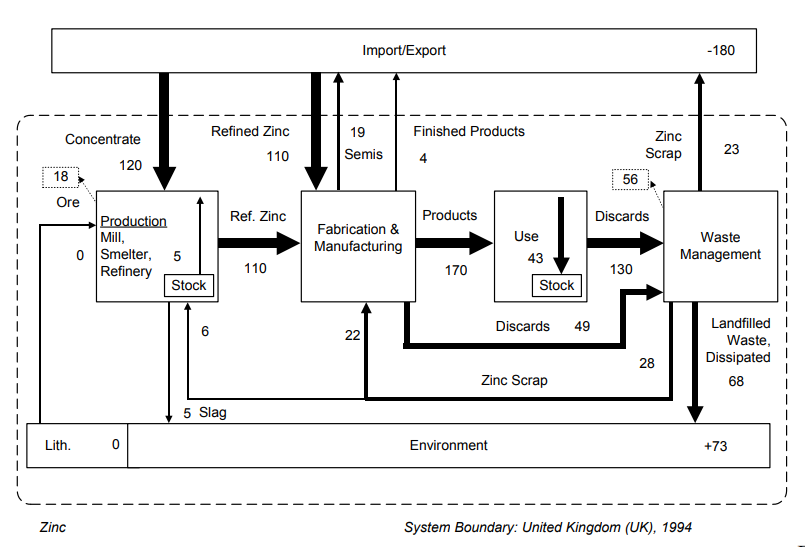
\includegraphics[width=\linewidth]{images/zinc_uk_mfa.png}
    \caption{MFA block flow diagram showing the cycle of Zinc through the UK in 1994 in Gg/year. Processes are denoted as boxes and stafs as arrows. The width of the magnitude of the stock or flow.}
    \label{fig:zinc_uk_mfa}
\end{figure}

The MFA data is first adapted to fit with UMIS. Each process is split into a transformation and distribution process with stocks residing on transformation processes. The lithosphere process and its outflow are omitted as the outflow quantity is zero. The small boxes connected to the Use and Production processes refer to mass balancing where there is an unaccounted for difference between the amount of material entering a process and the amount leaving. These are modelled as a flow to a new transformation process.

To represent the stock and flow values their uncertainty must be characterised. Graedal et al. describe uncertainty in their study through data quality categories. They report that flows to the environment are of poor accuracy ($\pm 67 - 95\%$), whilst external inflow and outflows are of moderate accuracy ($\pm 33 - 67\%$). Assuming that all other flows are of high accuracy ($\pm 5 - 33\%$), we can model stocks and flows as normally distributed random variables with standard deviations as the midpoint in these confidence intervals. Flows that have been created from splitting processes, mass balance flows and the stock representing accumulation in the environment have been left to be inferred. Therefore, they have been characterised as an uninformative uniform distribution between $0$ and $500$. 

The adapted data from the diagram consists of a system with $18$ processes and $22$ stafs. It was entered into STAFDB-P and can be seen in Appendix \ref{app:stafdb_p_graedal}. The stocks and flows comprising the external inflows, internal stafs and external outflows are selected from STAFDB-P by their ID and used to construct a UMIS diagram. This is used to create a \texttt{UmisMathModel} object which initialises a mathematical model representation of the system. Posterior distributions for stock, flow, TC and CC values with calibrated uncertainty are then inferred by sampling from the model $5000$ times. Best estimates for parameters are obtained through MAP over the model.

\subsection{Graedal Example Results}
\begin{table}[h]
    \small
    \center
    \begin{tabular}{|l|l|l|}
        \hline
        \textbf{Parameter}              & \textbf{Graedal Value (Gg/year)} & \textbf{Bayesian inference Value (Gg/year)} \\ \hline
        Production – Mass Balance       & 18                     & 15.8                              \\ \hline
        Waste Management – Mass Balance & 56                     & 58.7                              \\ \hline
        Accumulation in Environment      & 73                     & 73.0                                \\ \hline
    \end{tabular}
    \caption{Values calculated by Graedal for 2005 Zinc Cycle in UK and by Bayesian inference accounting for uncertainty. The Bayesian inference values were inferred from uniform priors}
    \label{table:graedal_results}
\end{table}
Table \ref{table:graedal_results}, shows that the Bayesian inference estimates are close to the values calculated by Graedal. The reason for the slight difference between the inferred and Graedal mass balance values is likely due to the introduced uncertainty. The origin process for the mass balance flows are the distribution processes for Production and Waste Management. In splitting the processes into transformation and distribution we introduced new flows leading into these distribution processes which have an uninformative uniform prior distribution. As there is large uncertainty in the values constraining the Mass Balance flows, their  posteriors have a corresponding large uncertainty. In contrast, the inferred Accumulation in Environment value is equal to Graedal's value which reflects the comparatively lower uncertainty of the values constraining it. The inferred posteriors can be seen in figure \ref{fig:mass_balance_posteriors}.

\begin{figure}[t]
    \centering
    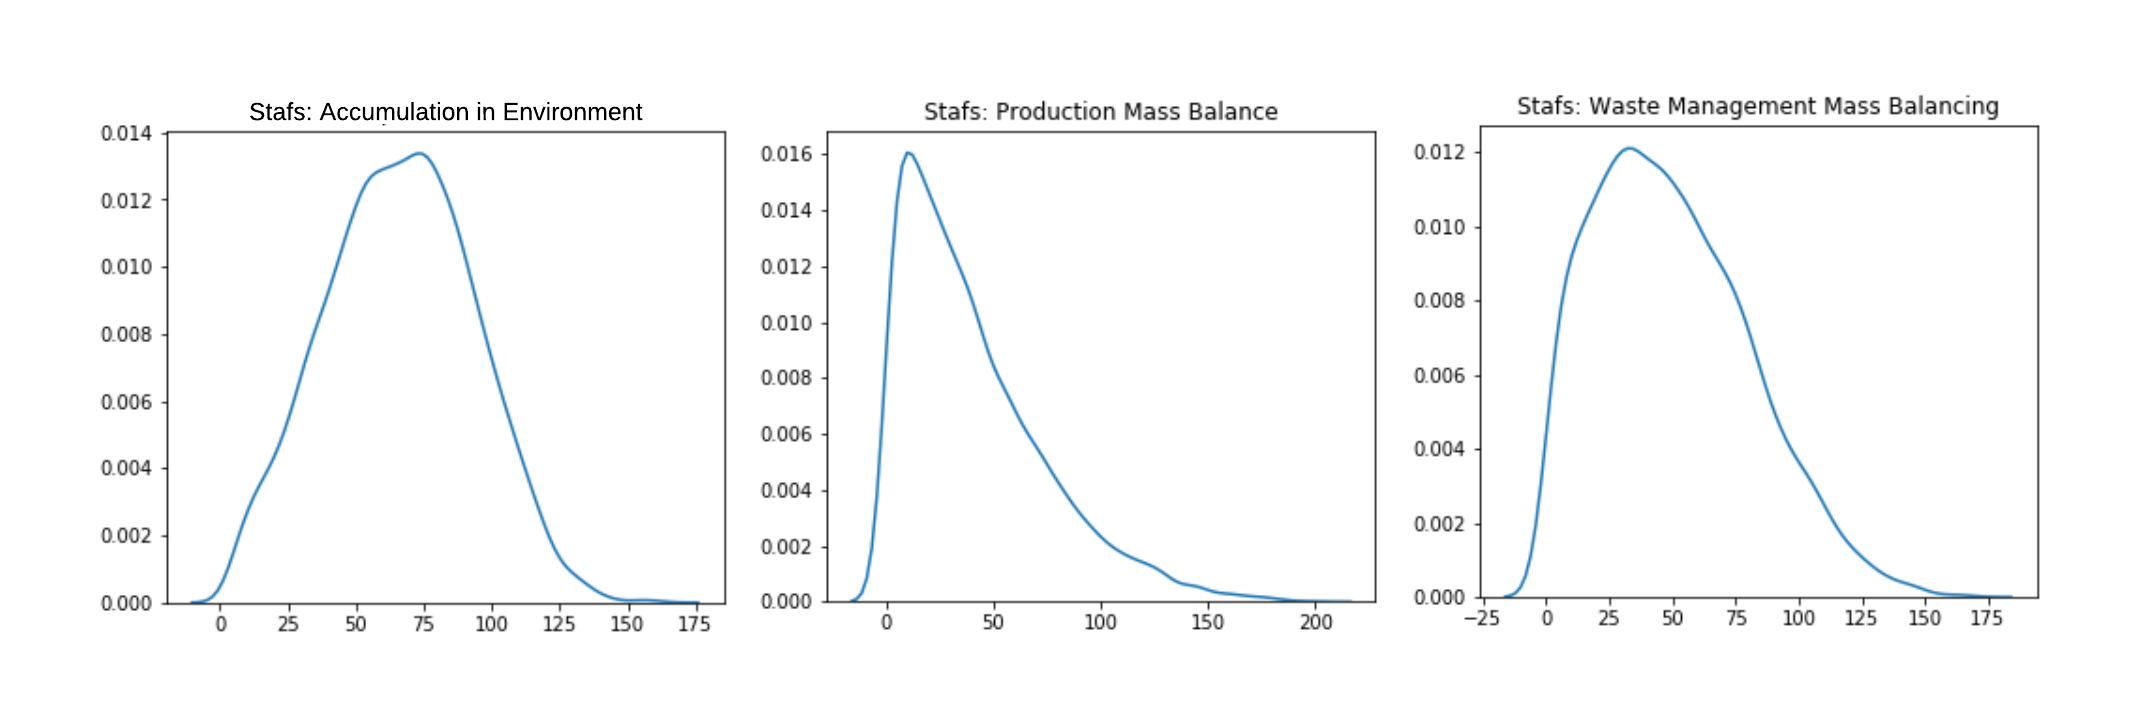
\includegraphics[width=\linewidth]{images/graedal_data_posteriors.png}
    \caption{Posterior distributions of Accumulation in Environment (left) Production Mass Balance (middle) and Waste Management Mass Balance (right)}
    \label{fig:mass_balance_posteriors}
\end{figure}


The inference of our model parameters as posterior distributions means that model results can be interpreted more reliably. For example, the model automatically infers the ratio of material going to stock in the Use process as well as its accompanying uncertainty (top right distribution in figure \ref{fig:graedal_posteriors}). If these values are being used to calculate indicators of resource availability or wastage as in Graedal's study, it is important to empirically calculate and report on the accompanying uncertainty of these values. Therefore it is useful to produce accurate, calibrated posterior distribution estimates as in figure \ref{fig:graedal_posteriors}.


% probability distributions describing the uncertainty of the ratio of stock in the Use process can be automatically calculated and observed as in figure \ref{fig:graedal_posteriors}
%. However, this result is a more informative measure than Graedal's mass balance value as it represents the range that the mass balance may take, and incorporates the uncertainty of the surrounding values. 
\begin{figure}[h!]
    \centering
    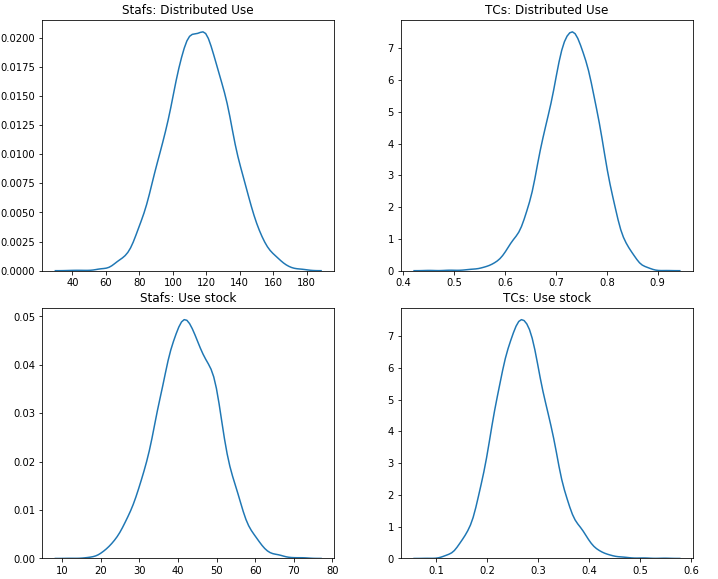
\includegraphics[width=0.5\linewidth]{images/graedal_posteriors.png}
    \caption{Posterior distributions of outflows from the Use transformation process and their transfer coefficients. Top: Flow from Use - Transformation to Use - Distribution. Bottom: Stock from Use - Transformation}
    \label{fig:graedal_posteriors}
\end{figure}

\section{Gaussian Error Propagation Example}
\label{sec:gauss_example}
Whilst the above example demonstrates that the Bayesian inference engine can calibrate uncertainties over UMIS systems, it does not guarantee that the reconciled posteriors are accurate. In \cite{cencic2016nonlinear}, Cencic characterises his model parameters as normally distributed random variables and performs least squares optimisation using model constraints to propagate error and reconcile data. By testing the Bayesian inference engine over the same model that Cencic used, we can determine whether the engine is reconciling data with normally distributed uncertainty correctly.

Cencic tests his algorithm on a small system with 5 mass flows and 3 internal processes. Uncertainty is characterised by true values and a confidence interval which correspond to the mean and standard deviation of a normal distribution. His system must be adapted as it has two external inflows to the first process which is not supported in UMIS. However, as only one of the flows has an associated uncertainty the two external inflows can be combined by summing the true values and keeping the first's confidence interval. The system is converted into the UMIS diagram seen in figure \ref{fig:cencic_system} and fed into \texttt{UmisMathModel}.

\begin{figure}[h!]
    \centering
    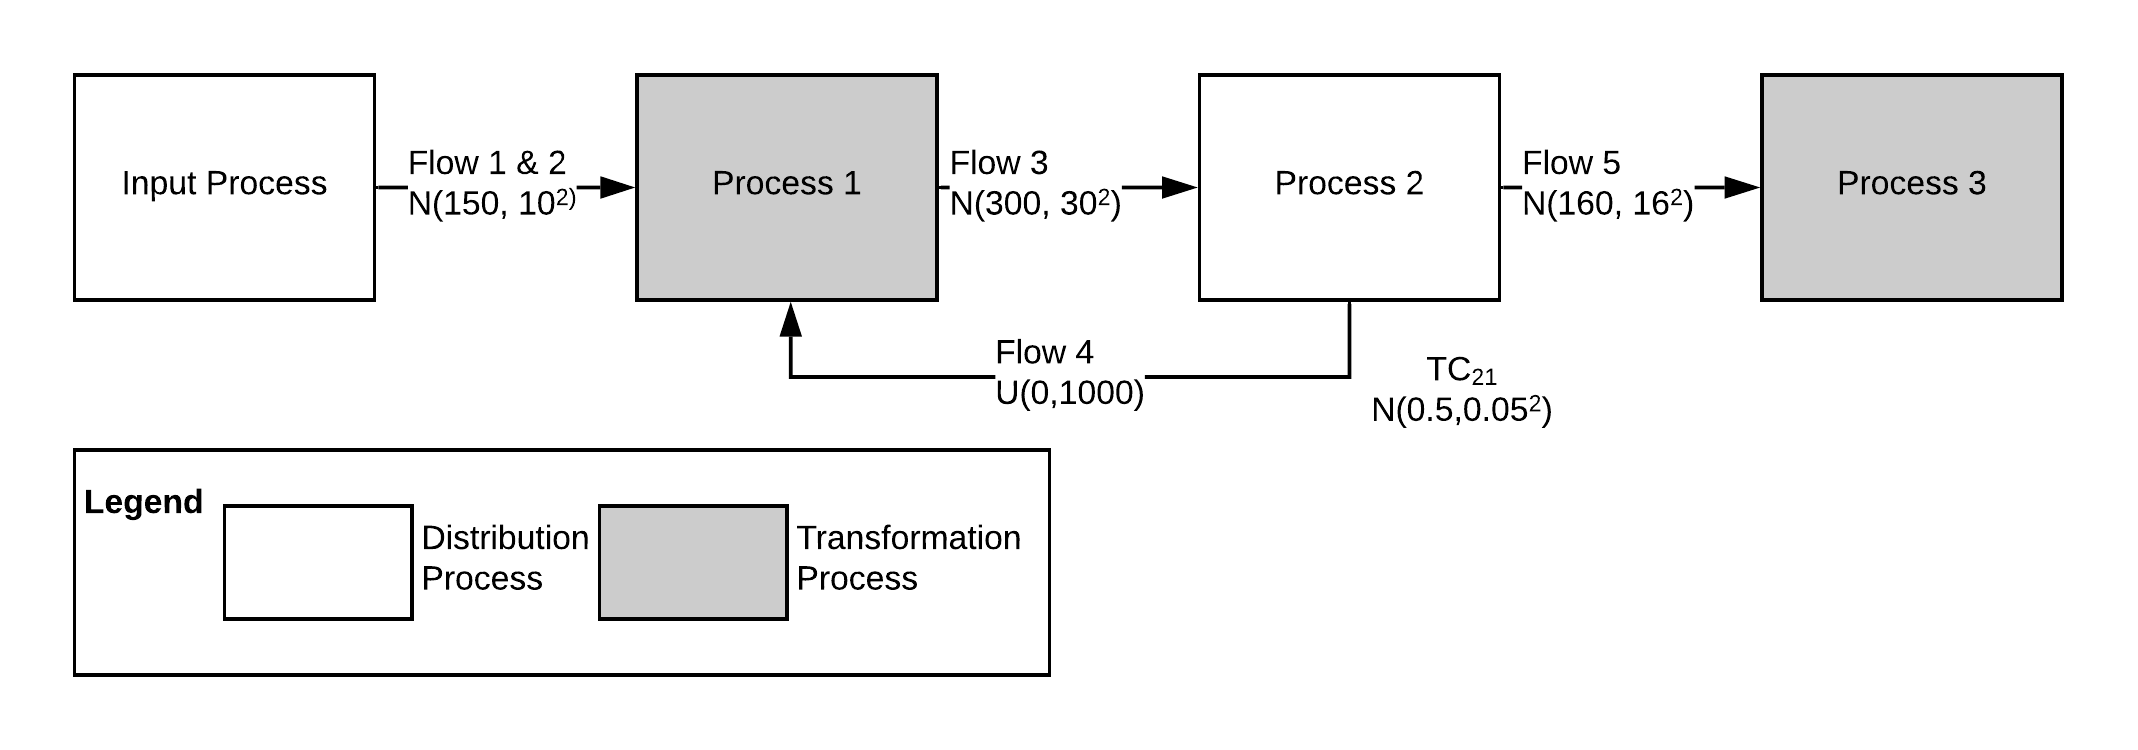
\includegraphics[width=\linewidth]{images/cencic_system.png}
    \caption{UMIS representation of system used in evaluation of \cite{cencic2016nonlinear}. $N(\mu, \sigma^2)$ denotes a value uncertainty equivalent to a normally distributed random variable with mean $\mu$ and standard deviation $\sigma$. $U(l, u)$ denotes a uniformly distributed random variable with lower and upper bound $l$ and $u$}
    \label{fig:cencic_system}
\end{figure}

Cencic's system also has an observation of a distribution process TC as $N(\mu=0.5,\sigma^2=0.05^2)$. As the Bayesian inference engine only supports priors for distribution TCs expressed as shares of a Dirichlet distribution this must be converted. Fortunately this is relatively simple as the process has two equivalent TCs. The resultant Dirichlet distribution is known as a Beta distribution whose standard deviation is given by $\sigma= \sqrt{\frac{\alpha_1\alpha_2}{(\alpha_1 + \alpha_2)^2(\alpha_1+\alpha_2 + 1)}}$, where $\alpha_1, \alpha_2$ are the shares. Therefore where $\alpha_1 = \alpha_2 = 49.5$, the resultant random variables are both equivalent to $N(\mu=0.5,\sigma=0.05^2)$. By adding prior observations of $TC_{21} = TC_{23} = 49.5$ we can create an equivalent system.

% can show proof of distribution
\subsection{Gaussian Error Propagation Results}
\label{sec:gauss_results}
The resultant mathematical model is sampled from $3000$ times and MAP is performed over it. The parameter standard deviations and best estimates are extracted and shown in table \ref{table:cencic_results}.

\begin{table}[h]
\begin{tabular}{|l|l|l|l|l|l|l|}
\hline
\textbf{Parameter} & \textbf{Prior Mean} & \textbf{Prior SD} & \textbf{GEP Mean} & \textbf{GEP SD} & \textbf{BI MAP Estimate} & \textbf{BI SD} \\ \hline
Flow 1 \& 2   & 150                 & 10                & 152.4                & 7.9                & 152.4                    & 7.9            \\ \hline
Flow 3             & 300                 & 30                & 302.4                & 22.6               & 302.4                    & 22.5           \\ \hline
Flow 4             & ?                   & ?                 & 150                  & 21.2               & 150                      & 20.9           \\ \hline
Flow 5             & 160                 & 16                & 152.4                & 7.9                & 152.4                    & 7.9            \\ \hline
TC21               & 0.5                 & 0.05              & 0.5                  & 0.04               & 0.5                      & 0.04           \\ \hline
\end{tabular}
\caption{Results from data reconciliation over Cencic's evaluation system using Guassian Error Propagation (GEP) and our Bayesian inference approach(BI). SD refers to the standard deviation of the distributions}
\label{table:cencic_results}
\end{table}

All parameter values have had their estimated value shifted and their uncertainty reduced. Notably, Flow 5 has been reduced from $160$ to $150$ which demonstrates the effect of the model constraint in its transfer coefficient of $0.5$. Most of the parameter values have been reconciled to the same values as that of Cencic's reconciliation. The only difference is that of the inferred parameter Flow 4. In Cencic's system this is an unknown value and is calculated from the parameters after reconciliation. My approach models it as having its own prior uniform distribution which will affect the posterior inferred distribution slightly, however this difference is negligible and does not affect the true values. This test indicates the correctness of the inference engine over normally distributed values. As my approach does not rely on any assumptions of normal distribution and instead the calculation of probability and likelihood values, it is a further indication that the inference engine correctly reconciles values with different distributions.  

\section{Mixed Log-normal and Normal Example}
A key feature to the Bayesian inference engine over the Gaussian Error Propagation approach is that it is agnostic to the probability distributions of the model parameters. To evaluate this we re-characterise the uncertainty in Cencic's evaluation system to contain both normal and log-normal distributions. The Bayesian inference engine then calculates posteriors that incorporate the uncertainty of each parameter. Table \ref{table:lognormal_changes} shows the new prior representations of the parameters in the model. The TCs are not provided with a prior observation so therefore just use the default prior, that of variables in a Dirichlet distribution where each value between 0 and 1 is equally likely.

\begin{table}[]
\center
\begin{tabular}{|l|l|l|}
\hline
\textbf{Parameter} & \textbf{Distribution} & \textbf{Parameters} \\ \hline
Flow 1 \& 2        & Lognormal             & $\mu=ln(150), \sigma=0.25$ \\ \hline
Flow 3             & Normal                & $\mu=300, \sigma=30$       \\ \hline
Flow 4             & Uniform               & lower=$0$, upper=$1000$ \\ \hline
Flow 5             & Lognormal             & $\mu=ln(160), \sigma=0.25$ \\ \hline
TC$_{21}$         & Dirichlet             & $\alpha=1$             \\ \hline
TC$_{23}$         & Dirichlet             & $\alpha=1$             \\ \hline
\end{tabular}
\caption{Prior distributions of parameters for log-normal example.}
\label{table:lognormal_changes}
\end{table}

\subsection{Mixed Log-normal and Normal Example Results}
\label{sec:mixed_example}
The resultant mathematical model is sampled from $3000$ times and the posteriors extracted. The prior and posterior distributions of Flows 3, 4 and 5 as well as TC$_{21}$  can be seen in figure \ref{fig:lognormal_posteriors}. The less certain prior distributions of Flow 4 and Flow 5 and TC$_{21}$ have had their uncertainty reduced drastically. Flow 3's tighter distribution has been changed to a lesser extent. This indicates that the Bayesian inference engine still reconciles data, regardless of how their prior distribution is characterised. Furthermore, it appropriately alters parameter values according to how uncertain their priors are. As can be seen from the top left graph in figure \ref{fig:lognormal_posteriors}, the Bayesian inference engine can also infer parameter values from extremely uninformative priors even when the provided uncertainties are characterised by different distributions. This demonstrates the inference engine's flexibility to various types of uncertainty characterisation.

\begin{figure}[]
    \centering
    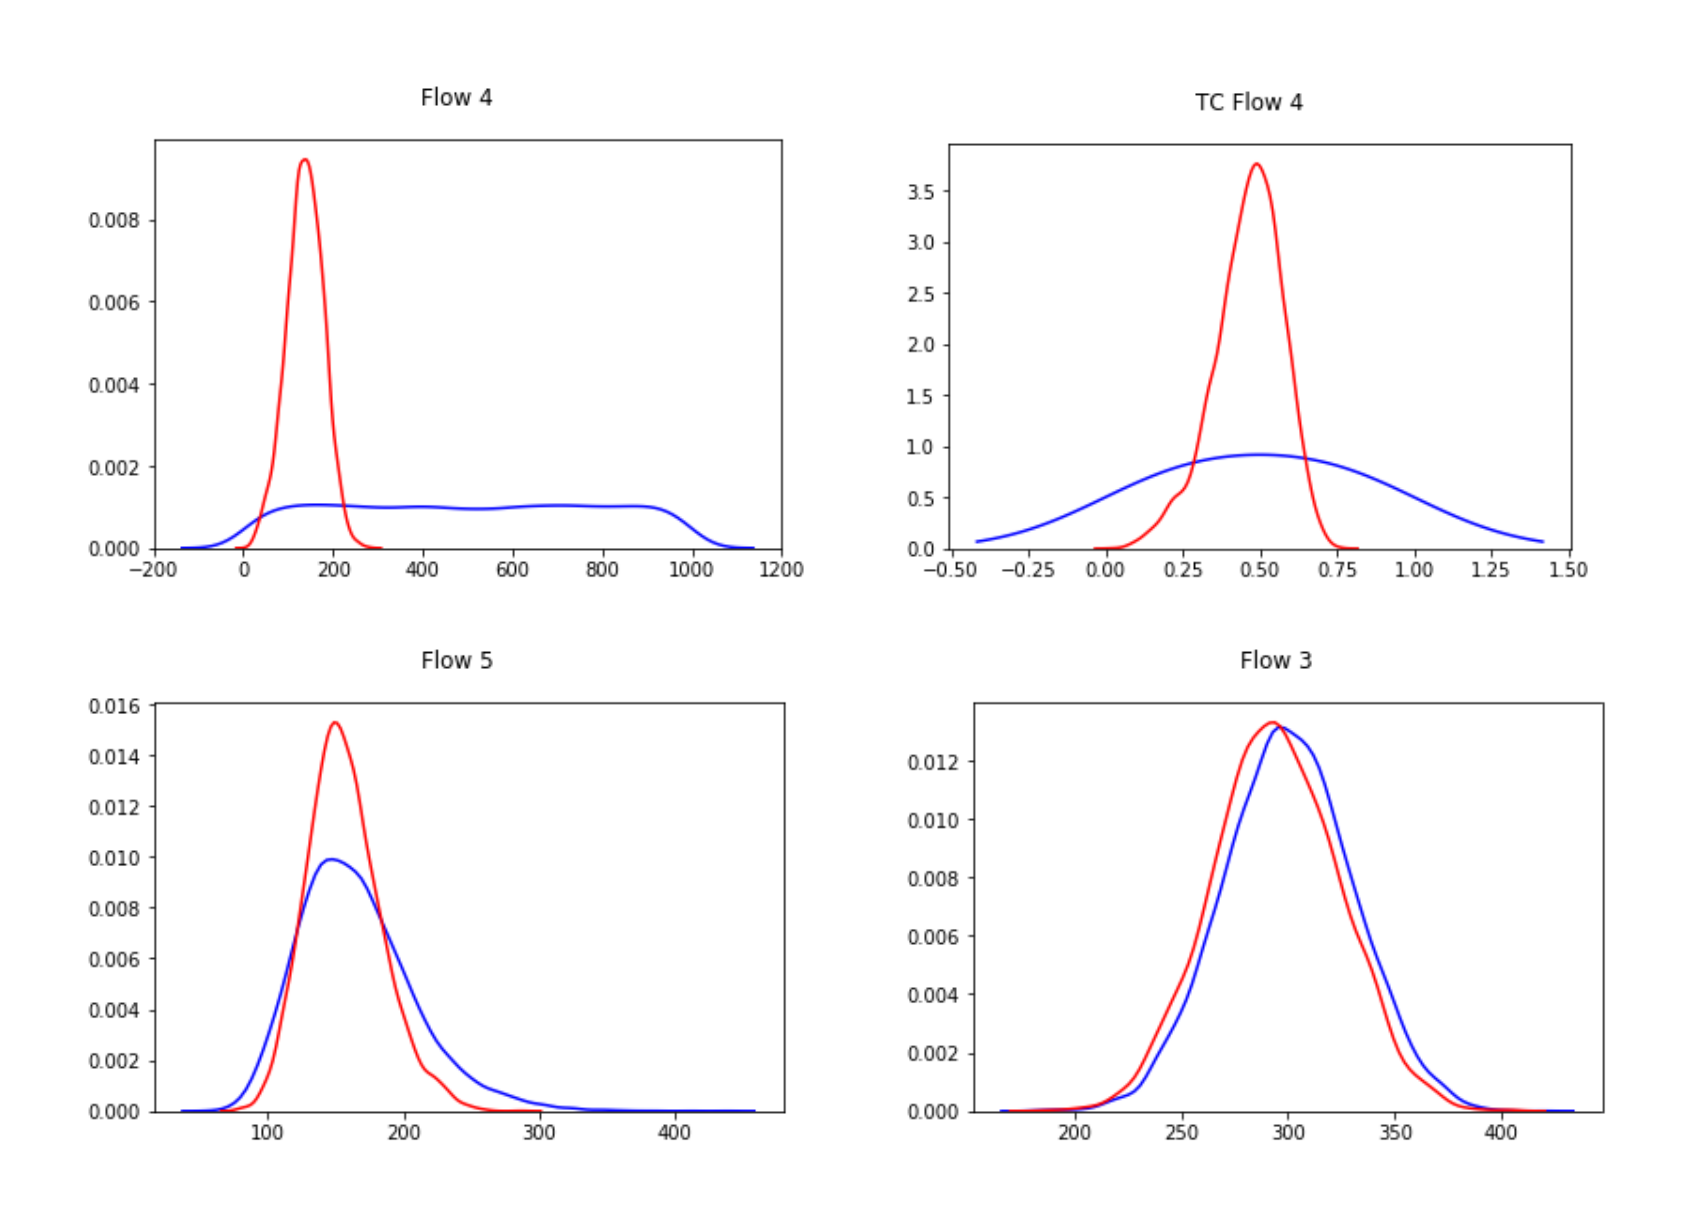
\includegraphics[width=0.66\linewidth]{images/lognormal_posteriors.png}
    \caption{Prior (blue) and posterior (red) distributions of model parameters after Bayesian inference. Top left: Flow 4's distributions. Top right: Flow 4's TC, TC$_{21}$'s distributions. Bottom left: Flow 5's distributions. Bottom right: Flow 3's distributions}
    \label{fig:lognormal_posteriors}
\end{figure}

\section{Concentration Coefficients Example}
\label{sec:cc_example}
Another feature of the Bayesian inference engine is that it can perform material reconciliation through the use of concentration coefficients. This allows for IE systems with composite materials to be balanced in terms of a single reference material. To demonstrate the engine's ability to deal with such systems, we adapt Cencic's system described in section \ref{sec:gauss_example} by using the flows of both a composite material and the reference material. We scale the mean values of the flows expressed as composite materials so that when reconciled they represent the same quantity of the reference material in Cencic's system. As we do not change the standard deviations, the resultant reconciled values are expected to be the same as that of in section \ref{sec:gauss_results}. To thoroughly test the system we express both a dependent parameter (Flow 5) and a free parameter (Flow 1 \& 2) in the composite material. The concentration coefficient is characterised as a normal distribution with mean $0.625$ and standard deviation $0.05$; we accordingly scale the unreconciled flows by multiplying by $1.6$. The new parameter prior values are shown in table \ref{table:conc_coeff_params}.

\begin{table}[]
\center
\begin{tabular}{|l|l|l|l|}
\hline
\textbf{Parameter}    & \textbf{Distribution} & \textbf{Parameters}  & \textbf{Material}  \\ \hline
Flow 1 \& 2           & Normal                & $\mu=256, \sigma=10$        & composite material \\ \hline
Flow 3                & Normal                & $\mu=300, \sigma=30$        & reference material \\ \hline
Flow 4                & Uniform               & lower=$0$, upper=$1000$  & reference material \\ \hline
Flow 5                & Normal                & $\mu=256, \sigma=16$        & composite material \\ \hline
TC$_{21}$            & Dirichlet             & $\alpha=49.5$           & N/A                \\ \hline
TC$_{23}$            & Dirichlet             & $\alpha=49.5$           & N/A                \\ \hline
Composite Material CC & Normal                & $\mu=0.625$, $\sigma=0.05$ & N/A                \\ \hline
\end{tabular}
\caption{Prior values for parameters in the Cencic evaluation system for the concentration coefficient example.}
\label{table:conc_coeff_params}
\end{table}

\subsection{Concentration Coefficients Example Results}
The model produced by the Bayesian inference engine is sampled from $3000$ times. To obtain best estimates of the parameter values, MAP is also performed over the model. The resultant reconciled data values can be seen in table \ref{table:conc_coeff_results}. The posterior values are very similar to the reconciled results in section \ref{sec:gauss_results} but have a slightly larger standard deviation (i.e uncertainty). This is a result of the added uncertainty introduced by the concentration coefficient. Nevertheless, the similarity between these reconciled results and that in section \ref{sec:gauss_results} demonstrate that the material reconciliation has been successful. Therefore the Bayesian inference engine can support MFA models that incorporate concentration coefficients. 

\begin{table}[]
\center
\begin{tabular}{|l|l|l|l|l|}
\hline
\textbf{Parameter} & \textbf{Prior Mean} & \textbf{Prior SD} & \textbf{BI MAP Estimate} & \textbf{BI SD} \\ \hline
Flow 1 \& Flow 2   & 256                 & 10                & 255.4                    & 9.45           \\ \hline
Flow 3             & 300                 & 30                & 307.8                    & 22.9           \\ \hline
Flow 4             & ?                   & ?                 & 149.8                    & 20.7           \\ \hline
Flow 5             & 160                 & 16                & 254.8                    & 14.1           \\ \hline
TC$_{21}$               & 0.5                 & 0.05              & 0.49                     & 0.04           \\ \hline
TC$_{23}$               & 0.5                 & 0.05              & 0.51                     & 0.04           \\ \hline
CC                 & 0.625               & 0.05              & 0.62                     & 0.04           \\ \hline
\end{tabular}
\caption{Reconciled values from the Bayesian inference (BI) engine for the concentration coefficient example system. SD refers to the standard deviation of the posterior distributions. The ? in the prior cells for Flow 4 denote a Uniform distribution with a lower bound of 0 and upper bound of 1000}
\label{table:conc_coeff_results}
\end{table}

\section{Evaluating Performance}
One of the disadvantages of the Bayesian inference approach is the length of time it takes to complete. Whilst performing MAP and constructing the mathematical model contribute to the run-time of the approach, they are negligible compared to the running time of the MCMC sampling. Therefore it is useful to examine what effect model properties have on the time taken to perform sampling. The time taken to take $3000$ MCMC samples from the models in the above examples have been recorded and can be seen in table \ref{table:example_times}. Additionally, the running time for a Cencic system with only log-normal uncertainties is included. These experiments were run on a laptop with a quad core 2.5Ghz CPU and 8 GB of RAM. The results indicate two factors that reduce the performance of the algorithm: the size of the system being modelled and the way the uncertainty is characterised.

\begin{table}[]
\center
\begin{tabular}{|p{4.5cm}|p{2cm}|p{2cm}|l|p{2cm}|}
\hline
\textbf{System Description}                                                         & \textbf{Number of Processes} & \textbf{Number of Stafs} & \textbf{Time taken (s)} & \textbf{Mean \mbox{Acceptance} Probability} \\ \hline
Gaussian Error \mbox{Propagation} Example system                                          & 3                            & 4                        & 35.3                    & 0.860                                \\ \hline
Concentration Coefficient \mbox{Example} system                                           & 3                            & 4                        & 53.9                   & 0.846                                \\ \hline
Log-normal and Normal \mbox{Example} system                                               & 3                            & 4                        & 57.0                      & 0.853                                \\ \hline
Cencic evaluation system with flows characterised only as log-normal distributions & 3                            & 4                        & 277.4                   & 0.796                                \\ \hline
Graedal MFA Example \mbox{system}                                                         & 18                           & 22                       & 477                     & 0.864                                \\ \hline
\end{tabular}
\caption{Time taken for the Bayesian inference engine to complete MCMC sampling over different systems}
\label{table:example_times}
\end{table}

\subsection{Effect of Uncertainty on Performance}
\label{sec:uncertainty_performance}
The top three rows of table \ref{table:example_times} shows the effect of varying the method of uncertainty characterisation on the run time of MCMC sampling. Of particular interest is the large increase in run time when characterising with only log-normal distributions. As there is no difference in the model shape, this indicates that the increase in run-time is due to the rate of proposal acceptance instead of the calculation of dependent parameters or drawing proposal values. As discussed in section \ref{sec:bayesian_inference}, the acceptance probability is calculated from a proposal of the free parameters. This proposal is used to calculate values for dependent parameters. The acceptance probability is then proportional to the likelihood of these dependent values coming from their prior distributions. Table \ref{table:example_times} indicates that the NUTS sampler does not propose as likely parameter values for models with log-normal distributions. This leads to more samples being rejected and a longer run-time. Therefore systems with log-normal distributions will accordingly have longer run-times as their samplers will have a lower acceptance rate.

\subsection{Effect of Model Size on Performance}
The second factor affecting the run time of the inference engine is the number of parameters in the model, more specifically the number of random variables. Evidence of this can be seen in the run time of the Graedal MFA Example system. Despite its mean acceptance probability being higher than all others, it has the longest running time. Therefore it is the computation cost per proposal for the system causing this delay, rather than the rejection of proposals. 

There could be a number of reasons for the increased computational cost of this model. One is that the increased number of free parameters means that more values must be drawn from the proposal distribution. Another is that due to the increased size of the matrices in the resultant mathematical model, the operations to calculate the dependent variables take more time. In particular the matrix inversion operation is of $\Omega(n^2log(n))$ time complexity \cite{tveit2003complexity} where $n$ is the number of processes in this case. Therefore an increase in the size of the model will result in an accordant increase in run time.

The final culprit may be in the increase in the number of stafs. Each staf correlates to a new likelihood term in the model; calculating this will also increase the run time. In \cite{lupton2018incremental}, Lupton et al. follow an incremental approach where they define a system of $72$ processes and $27$ flows. The approach is described as incremental as the uncertainty of the entire system is reduced by adding observations of flow values in stages. As a result different stages of their model have different numbers of likelihood terms. On running a stage with no observations and therefore no likelihood term, sampling $2000$ times took 3 minutes and had a mean acceptance probability of 0.8265. When sampling only $500$ times from a model with 27 observations, the inference took over an hour with a mean acceptance probability of 0.795. Whilst the decrease in acceptance probability may have had some effect on the run-time, it is not enough to account for such a large increase. Instead, this demonstrates that the number of likelihood terms incorporated into the model drastically increases its running time.

To further explore the relationship between system size and run time, we conducted an experiment where we varied the size of the input system and recorded the time taken to draw $3000$ samples from the posterior. The input system size is varied by concatenating multiple Cencic evaluation systems into the same diagram. The resultant run times and acceptance probabilities can be seen in figure \ref{fig:performance_graph}. The results show that the time taken for the inference engine to complete grows rapidly with the size of the system. A spike in running time can be observed at a size $44$ stafs. This could be due to the way the Pymc3 sampler is optimised in its back-end, where an improvement from parallelisation may come into effect.

The size of the system had a slight inverse effect on the acceptance rate of proposals, however this effect is not great enough to account for the large increase in run time. This tells us that the Bayesian inference engine run time is largely dependent on system size. This run time reached $15$ minutes in a system containing $60$ stafs even with relatively high rates of proposal acceptance. Therefore we suggest a usable system size of $60$ stafs. To put this size in context of real IE studies, the case study used by Lupton et al. in \cite{lupton2018incremental} contained $73$ observable flows, the study by Gottschalk et al. \cite{gottschalk2010probabilistic} contained $30$ and the Graedal study in section \ref{sec:graedal_example} contains $22$ stafs, therefore the engine is usable for most studies. For cases with larger systems, more powerful computers or even cloud computing resources could be leveraged to offset this run time.

\begin{figure}
    \centering
    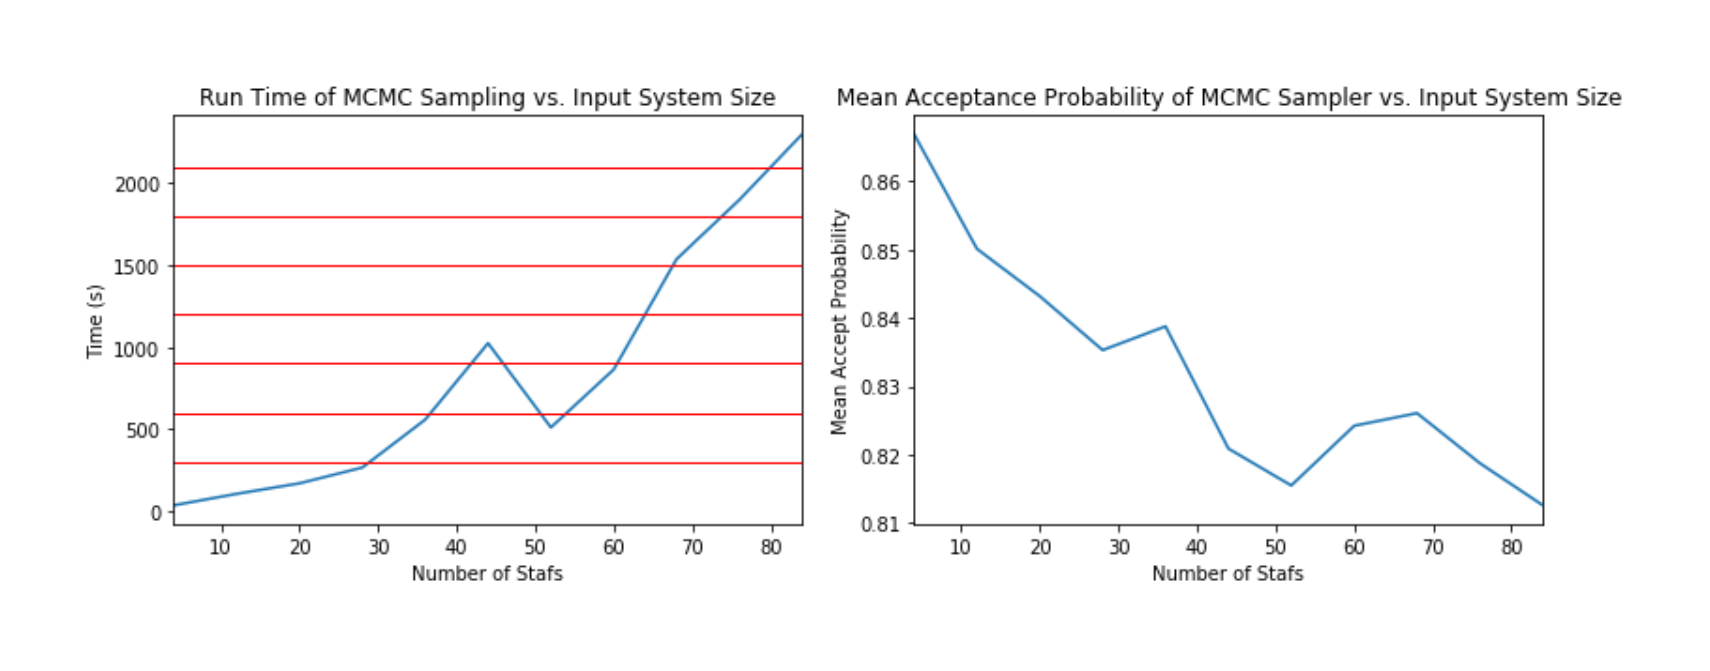
\includegraphics{images/performance_graphs.png}
    \caption{Graphs showing the relationship of input system size on MCMC sampler run time (left) and MCMC sampler mean acceptance probability (right). The red lines in the left image correlate to 5 minute intervals}
    \label{fig:performance_graph}
\end{figure}


\section{Failure Cases}
The Bayesian inference engine is fairly successful provided the described system is a legitimate UMIS diagram and supplied probability distributions are valid. In cases where the supplied parameters to the system do not agree with the mass balance constraints, the time taken for the posteriors to be drawn will be greatly increased due to a much lower acceptance probability for drawn samples. In this occasion, the resultant distributions will be unhelpful but still formed of acceptable values under the model constraints. Whilst estimating the posteriors is reliable, estimating best estimates for parameters under MAP is not. MAP failed in cases where two stafs connected to the same process required material reconciliation and in cases where all parameters were defined through log-normal distributions. I was unable to determine the specific cause of this.


\begin{comment}
{\bf A topic-specific chapter, of roughly $15$ pages} 
\vspace{1cm} 

\noindent
This chapter is intended to evaluate what you did.  The content is highly 
topic-specific, but for many projects will have flavours of the following:

\begin{enumerate}
\item functional  testing, including analysis and explanation of failure 
      cases,
\item behavioural testing, often including analysis of any results that 
      draw some form of conclusion wrt. the aims and objectives,
      and
\item evaluation of options and decisions within the project, and/or a
      comparison with alternatives.
\end{enumerate}

\noindent
This chapter often acts to differentiate project quality: even if the work
completed is of a high technical quality, critical yet objective evaluation 
and comparison of the outcomes is crucial.  In essence, the reader wants to
learn something, so the worst examples amount to simple statements of fact 
(e.g., ``graph X shows the result is Y''); the best examples are analytical 
and exploratory (e.g., ``graph X shows the result is Y, which means Z; this 
contradicts [1], which may be because I use a different assumption'').  As 
such, both positive {\em and} negative outcomes are valid {\em if} presented 
in a suitable manner.
 
 - Evaluation - turn graedal diagram into UMIS diagram
  - Evaluation - Lognormal, does that work
\end{comment}

% -----------------------------------------------------------------------------

\chapter{Conclusion}
\label{chap:conclusion}

\section{Project Features and Limitations}
The primary purpose of this thesis is to develop a method of calibrating uncertainty over UMIS structured systems. Pythonic representations of UMIS data were designed and an accompanying Bayesian inference engine was developed to reconcile the uncertainty of parameters over MFA systems. The predominant features of the engine is that it aligns with UMIS structured data, is flexible to the characterisation of uncertainty and can perform material reconciliation. These capabilities separate it from the work of Cencic et al. \cite{cencic2016nonlinear, cencic2015general, cencic2018data}, Lupton et al. \cite{lupton2018incremental} and Gottschalk et al. \cite{gottschalk2010probabilistic}. The accuracy of the engine is demonstrated in section \ref{sec:gauss_example}, where normally distributed uncertainty values are correctly calibrated, achieving the same results as Cencic's Gaussian Error Propagation approach. 

Section \ref{sec:graedal_example}, demonstrates the engine's ability to propagate uncertainty through UMIS structured systems with a real world MFA case study. The study was stored in a prototype STAFDB implementation and extracted into the UMIS Python objects with no loss of information. Unknown values are correctly inferred with some slight deviance and calibrated posterior distributions are produced. This method of propagating uncertainty is useful as it provides reconciled distributions for all model parameters. Therefore if these parameters are then used to calculate study results, Monte Carlo simulations can be used to propagate the reconciled uncertainty of the parameters into model results.

There are a few limitations of the current implementation of the Bayesian inference engine when dealing with UMIS structured data. Firstly the current implementation only deals with net stock values and ignores data concerning total stocks. The engine will require further development to handle systems that are concerned with total stock levels as this requires knowledge of the total stock levels in the previous time-frame. Furthermore the system currently ignores the unit that staf data is stored in and assumes that the unit does not change for each value. This could be rectified through unit reconciliation where staf values are multiplied by a factor to ensure that data is all in the same unit. As unit scale factors would be constant and therefore not introduce any new model parameters, it is omitted from this thesis.

% TODO future work would be adapting it for the real STAFDB once it is made
% By propagating uncertainty over UMIS structured data, each staf is required to have at least one value even if it is unknown. This is necessary as the stafs that are used for free parameters (input flows and incoming stocks) need to have a prior distribution for proposals to be sampled from. Unknown parameters are instead modelled as wide uniform distributions which adds additional uncertainty 
One novel feature of the system is that it supports material reconciliation. Concentration coefficients converting materials into the reference material can be expressed through random variables or as constants and allow for systems describing the metabolism of composite materials to be mass balanced. Evidence for this is found in section \ref{sec:cc_example}.

The engine's flexibility in dealing with uncertainty characterisation is demonstrated in section \ref{sec:mixed_example}. As discussed in chapter \ref{chap:context}, uncertainty in IE studies can be characterised in various ways. Therefore it is important to allow for their representation through any type of distribution. The framework developed by Lupton et al. allows for the characterisation of input flows as uniform and normal distributions and internal and external staf values through normal distributions only. TCs are also represented through a normal distribution for transformation processes, or as a parameters in a Dirichlet distribution for distribution processes. This has been extended to support normal, log-normal and uniform representations for transformation TCs and all staf values.

Distribution TCs remain represented by Dirichlet distributions which leads to limitations when trying to incorporate prior knowledge of their values into the model. We were fortunate that in section \ref{sec:gauss_example}, the Cencic evaluation system had a TC prior that could be represented by a Dirichlet prior relatively simply. However in the general case it is difficult to determine the exact $\alpha$ values to correctly represent prior knowledge of the TC. Another issue is that the way prior parameter information for distribution TCs is supplied to the Bayesian inference engine is not in line with its behaviour. Distribution TCs are represented by an \texttt{Uncertainty} object but the distribution information of the object is ignored and only the mean used as a $\alpha$ value for the Dirichlet distribution. To ensure that the behaviour of distribution TCs is the same as all other parameters in the model it would be better to represent them as uniform, normal and log-normal TCs, and ensuring that the TCs of a distribution process sum to 1.

Whilst the engine's ability to produce posterior samples was robust to the characterisation of uncertainty, its ability to estimate the most likely model parameters through MAP was not. As the mean of the posterior distributions is not always guaranteed to be its most likely value, a different approach must be used. A solution could be found in converting the samples into a histogram and finding the mode. A procedure for selecting a suitable bucket size for the histogram would need to be developed.

One potential issue in the Bayesian inference engine is the omission of the Lebesgue measure of the constrained posterior ($V(\bm{w})$) referenced in equation \ref{eq:cencic_posterior}. Cencic et al. argue that this must be incorporated into the acceptance probability of the sampler in order to ensure that the posterior being sampled from is invariant when the model contains non-linear constraints. The documentation of Pymc3 makes mention of Jacobian terms but is unclear as to whether it automatically incorporates the Jacobian of random variable transformations (and therefore the Lebesgue measure) when sampling from the posterior. However, as Lupton et al. make no mention of this in \cite{lupton2018incremental}, this suggests that it is implicitly accounted for. Furthermore, the evaluation in section \ref{sec:gauss_example} infers the correct posteriors in a model with non-linear constraints which suggests that the Jacobian terms are included.

A useful result of the inference engine would be a measure of the cohesion of the model. This is a value the degree to which the observed values of the parameters agree with each other. This is useful as it indicates whether the system may need to be redesigned or whether the observed values are accurate. In the fuzzy set approach this is implemented by measuring how much the membership functions overlap for each fuzzy set representing the same parameter. This is an informative approach as it describes exactly which data points may not agree and can highlight where flaws may reside in the model. The Bayesian inference approach does not provide a fully equivalent measure. The mean acceptance probability could be used as an indicator of how likely the proposed parameters are and therefore the how well the free parameter priors agree with the dependent priors, but it does not describe which parameters specifically were found to be unlikely. The mean acceptance probability is also affected by the size of the system, and therefore is not a strong measure of the cohesion of the system. An alternative approach could be in examining how far expected values have been reconciled from their prior distributions as suggested in \cite{cencic2008material} for the Gaussian Error Propagation approach.

% Maybe reconciliation distance
\section{Future Work}
The approach in this thesis describes a technique for calibrating the uncertainty of parameters in static MFA systems using UMIS structured data. There are a number of areas which would fully establish this approach to be useful in terms of research. 

\subsubsection{Divergent Disaggregation}
Whilst this thesis has used UMIS as a basis for how the model data should be structured, there is still an integral aspect of UMIS that has not yet been addressed, the treatment of divergent disaggregation. As UMIS unifies data from across a variety of studies, UMIS diagrams can describe the same aspects of a system in different ways. This is known as divergent disaggregation. Therefore the same physical material could be described twice. In order to ensure that the same physical data is not counted twice in a diagram, UMIS provides a method for storing how processes, materials and spaces have been disaggregated. In our UMIS Python objects we have parent and \texttt{is\_separator} fields for accommodating this information but have implemented no technique for ensuring that double counting does not occur. For the inference engine to be used across real UMIS data it would therefore need to validate stock and flow data to ensure that it does not count real physical data twice.

In addition, this implementation has been based of a prototypical version of STAFDB as the original is not yet publicly available. To fully examine this approach's suitability for UMIS data, the UMIS Python objects will have to be created directly from STAFDB once it is available.

\subsubsection{User Interface}
When conducting the Graedal case study evaluation (section \ref{sec:graedal_example}, it became apparent that describing MFA systems in terms of records in STAFDB-P is a difficult and time consuming task. With no way to visualise the system being constructed it is easy to make mistakes in the system structure and difficult to validate the result. IE tools such as OMAT from the Metabolism of Cities project \cite{MetabolismOfCities}, Stan \cite{cencic2008material} and OpenLCA provide graphical user interfaces for creating static MFA and LCA models. Similarly to the intention of STAFDB, OpenLCA links with LCA databases, allowing for data to be shared across studies. It would be advantageous to have a similar user interfaces that allow for UMIS diagrams to be built graphically, using user inputted data and data from STAFDB. The Bayesian inference engine could then be used to calibrate uncertainty across these user defined systems.

\subsubsection{Further Distributions}
The Bayesian inference engine currently supports prior knowledge of model parameters characterised as normal, log-normal or uniform distributions. This is sufficient to represent uncertainty of data values calculated from data quality scores \cite{laner2016novel}, however for full flexibility other distributions should be supported. To obtain parity with the LCA database EcoInvent \cite{wernet2016ecoinvent}, it should be possible to model prior knowledge of data values through trapezoidal and triangular distributions. These distributions are not implemented by Pymc3, however the library does allow for developing custom distributions if methods for sampling from the distribution and calculating likelihood are provided.

\subsubsection{Dynamic MFA}
The Bayesian inference engine implemented in this paper operates over static MFA systems; systems that describe the stock and flow of material over a specific time snapshot. Dynamic MFA is an area of IE study that looks at the change in stocks and flows in a system over a series of time snapshots \cite{müller2014modeling}. This can incorporate new equations that use time and lifetime coefficients as parameters to predict future stock and flow values. Dynamic MFA studies are built on multiple static MFA studies of the same system but over different time snapshots. Therefore the Bayesian inference engine could compliment a dynamic MFA tool by automatically calibrating uncertainty across static snapshots. The calibrated uncertainty of model parameters could then be propagated into dynamic MFA results. Pauliuk et al. have already developed ODYM, an open source tool for performing dynamic MFA modelling over stocks and flows data using its own data structure and database design \cite{odym}. An equivalent system that is based on UMIS structured data would be advantageous as it would allow for integration with STAFDB and therefore data from LCA and IOA studies.

\subsubsection{Calibrating Uncertainty with LCA and IOA}
The key benefit to UMIS is that it allows data from MFA, LCA and IOA to be structured in the same format. Our approach is designed to calibrate uncertainty across MFA models, therefore future engines would have to be developed to handle LCA and IOA studies. Little adaptation would be required to implement an engine for IOA as the system is described in terms of one material (money) and follows the same balancing constraints as MFA. LCA may require additional development.

LCA typically involves examining the environmental impact of a single product. This is done by modelling the life cycle of the product as independent unit processes with elemental flows (external outflows and inflows to the environment) and intermediate flows (flows between unit processes) \cite{heijungs2013computational}. As each process is treated as independent, intermediate flows that are seen as outflows of its origin process are usually in a different scale to their corresponding inflows to its destination process. Therefore each process is characterised by its own scaling factor so that all flows, both elemental and intermediate are in terms of a single reference unit of the product being assessed. Therefore in order to calibrate uncertainty across LCA studies, the uncertainty of parameters around each independent unit process would need to be calibrated. The reconciled uncertainty values can then be used in calculating scaling factors and model results. Bayesian inference has already been applied to LCA studies by Lo in \cite{lo2005quantifying} where prior information of model parameters were updated by real world measurements and findings from national statistics. An engine to automatically apply this technique to UMIS structured unit processes would be a useful method of automatically calibrating uncertainty across LCA models.

\section{Summary}
Industrial Ecology is a field that utilises a variety of methodologies to analyse socio-economic metabolism. In order to reconcile the results of these studies, UMIS has been proposed so that systems analysed by IOA, LCA and MFA studies can be represented in the same machine readable format. STAFDB is a database that has been designed to store the underlying data that comprise UMIS diagrams so that a variety of IE data can be stored in the same location. This is designed to make it simpler to collaborate on research, publish findings and validate results. In IE data the treatment of data uncertainty is an important consideration and it must be represented in findings. A number of statistical approaches exist to calibrate uncertainty across MFA models, this thesis focuses on a Bayesian approach which models the calibrated uncertainty values in an MFA model as latent posterior distributions. Monte Carlo Markov Chains are discussed as a method of sampling from these posterior distributions and avoiding the onerous task of calculating the marginal likelihood of a high-dimensional model.

A Bayesian inference engine that generalises a Bayesian inference approach to calibrating uncertainty over MFA models structured in UMIS diagrams is proposed. A Pythonic representation of UMIS was developed to represent the MFA systems. These are then used as input to the engine which converts the system into a mathematical model using Pymc3 and Theano operations. This posterior calibrated distributions of the MFA model parameters are then sampled from using a NUTS sampler provided by Pymc3. The posterior samples of model parameters can then be accessed from their corresponding UMIS \texttt{Stock} or \texttt{Flow} object.

To evaluate the resultant program a prototype of STAFDB was implemented. The Bayesian inference engine's capabilities at handling UMIS structured data as well as uncertainties characterised through normal, log-normal and uniform distributions were demonstrated successfully. A further demonstration was conducted to show the engine's ability to incorporate concentration coefficient parameters in the model as well. The running time of the system was evaluated and a cap of a system size of $60$ stafs was recommended for the system to remain usable. A link between unlikely characterisations of uncertainty and an increase in run time was also found. The main features of the project and its current limitations were discussed and future areas of development were highlighted. Predominantly, these focus on fully incorporating all features of UMIS into the program, improving the user experience and extending the system for Dynamic MFA, LCA and IOA models.

\begin{comment}
{\bf A compulsory chapter,     of roughly $5$ pages} 
\vspace{1cm} 

\noindent
The concluding chapter of a dissertation is often underutilised because it 
is too often left too close to the deadline: it is important to allocation
enough attention.  Ideally, the chapter will consist of three parts:

\begin{enumerate}
\item (Re)summarise the main contributions and achievements, in essence
      summing up the content.
\item Clearly state the current project status (e.g., ``X is working, Y 
      is not'') and evaluate what has been achieved with respect to the 
      initial aims and objectives (e.g., ``I completed aim X outlined 
      previously, the evidence for this is within Chapter Y'').  There 
      is no problem including aims which were not completed, but it is 
      important to evaluate and/or justify why this is the case.
\item Outline any open problems or future plans.  Rather than treat this
      only as an exercise in what you {\em could} have done given more 
      time, try to focus on any unexplored options or interesting outcomes
      (e.g., ``my experiment for X gave counter-intuitive results, this 
      could be because Y and would form an interesting area for further 
      study'' or ``users found feature Z of my software difficult to use,
      which is obvious in hindsight but not during at design stage; to 
      resolve this, I could clearly apply the technique of Smith [7]'').
\end{enumerate}

\end{comment}

% =============================================================================

% Finally, after the main matter, the back matter is specified.  This is
% typically populated with just the bibliography.  LaTeX deals with these
% in one of two ways, namely
%
% - inline, which roughly means the author specifies entries using the 
%   \bibitem macro and typesets them manually, or
% - using BiBTeX, which means entries are contained in a separate file
%   (which is essentially a databased) then inported; this is the 
%   approach used below, with the databased being dissertation.bib.
%
% Either way, the each entry has a key (or identifier) which can be used
% in the main matter to cite it, e.g., \cite{X}, \cite[Chapter 2}{Y}.

\backmatter

\bibliography{dissertation}

% -----------------------------------------------------------------------------

% The dissertation concludes with a set of (optional) appendicies; these are 
% the same as chapters in a sense, but once signaled as being appendicies via
% the associated macro, LaTeX manages them appropriatly.

\appendix
\chapter{}
\label{appx:example}

\section{STAFDB Entity Relationship Diagram}
\label{appx:stafdb_erd}
\begin{figure}[h!]
    \centering
    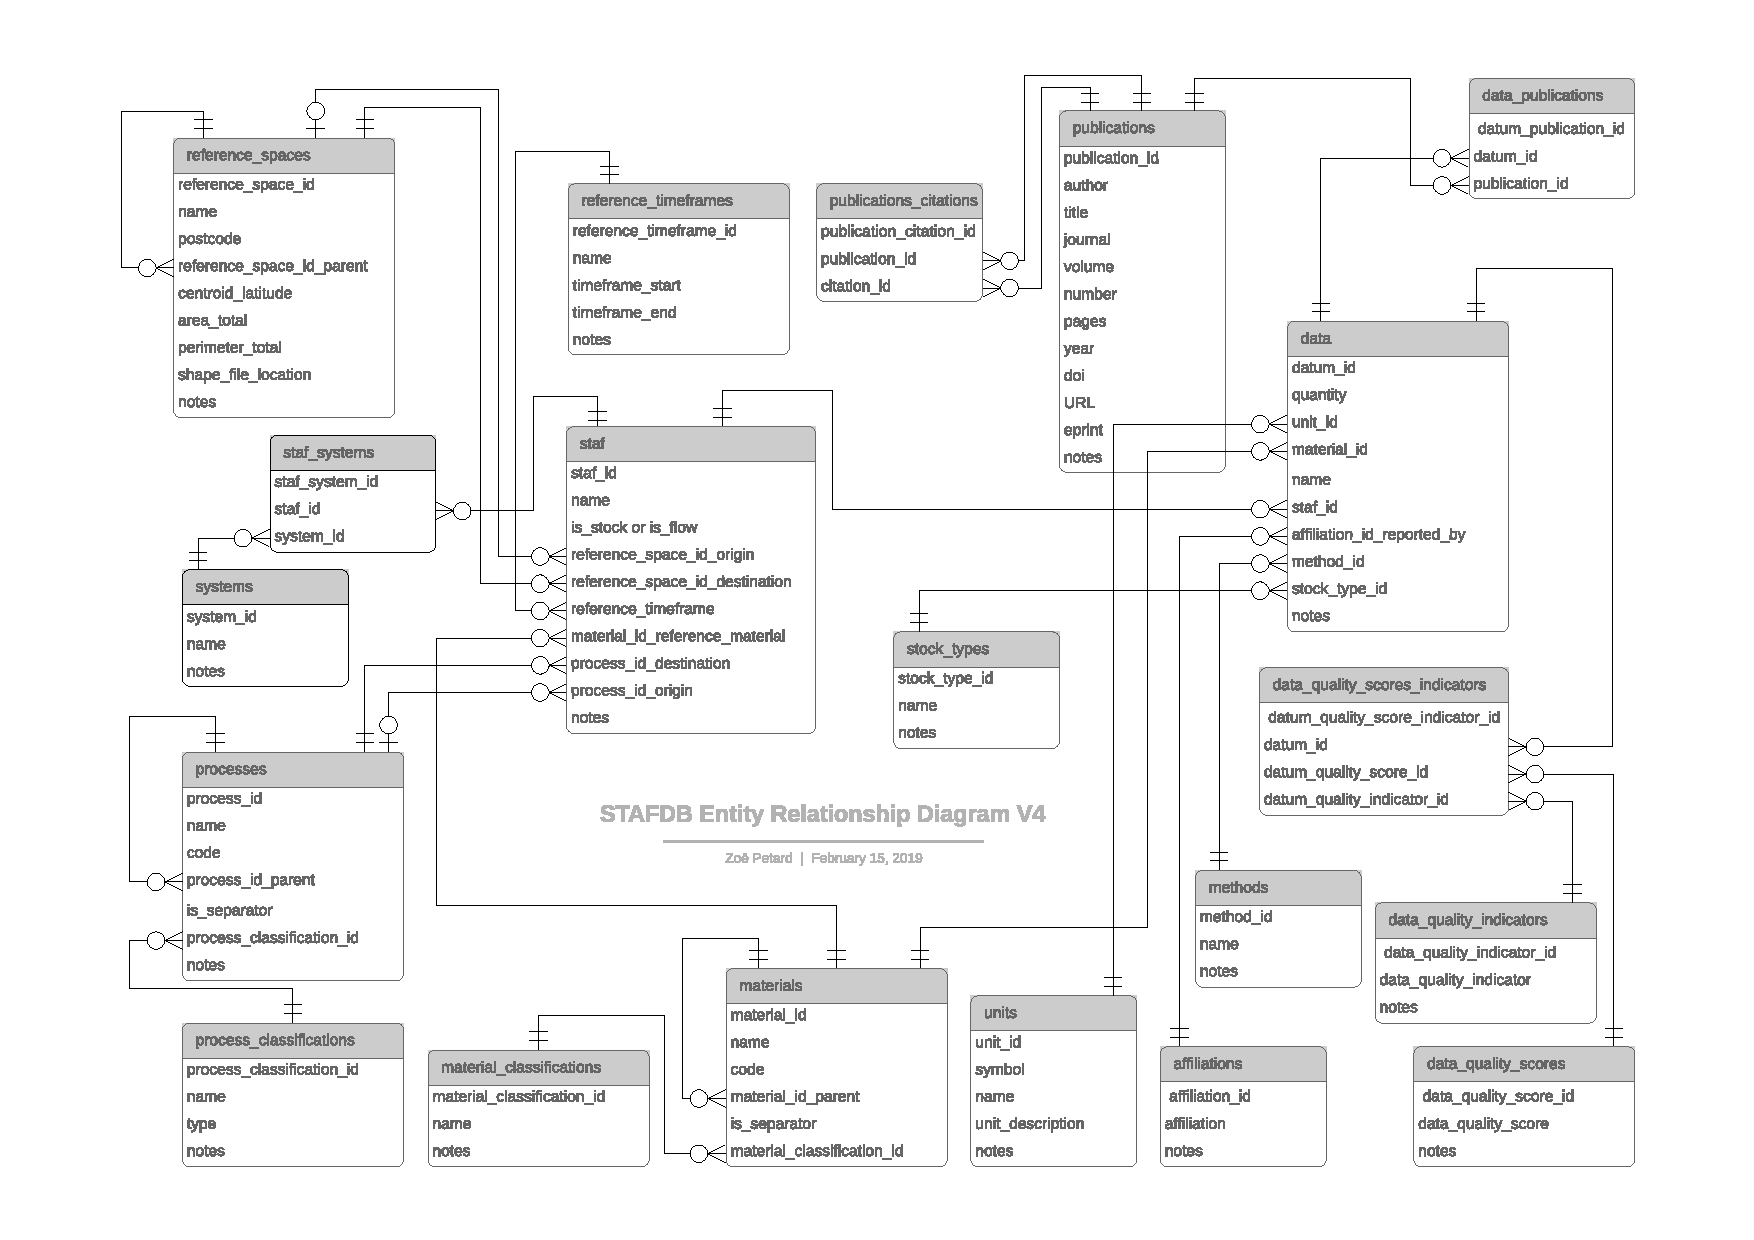
\includegraphics[width=\textwidth]{images/STAF_ERD_V4.pdf}
    \caption{Entity Relationship Diagram for in-progress STAFDB}
    \label{fig:stafdb_erd}
\end{figure}

\section{STAFDB-P for Graedal Test Example}
\label{app:stafdb_p_graedal}
% Please add the following required packages to your document preamble:
% \usepackage[normalem]{ulem}
% \useunder{\uline}{\ul}{}
\begin{table}
\center
\begin{tabular}{|l|p{4.5cm}|l|l|l|l|}
\hline
{ \textbf{process\_id}} & { \textbf{name}}                                  & { \textbf{code}} & { \textbf{process\_id\_parent}} & { \textbf{is\_separator}} & { \textbf{process\_type}} \\ \hline
1                          & Import                                               & -----               & None                               & False                        & Distribution                 \\ \hline
2                          & Production: Mill, Smelter, Refinery – Transformation & -----               & None                               & False                        & Transformation               \\ \hline
3                          & Production: Mill, Smelter, Refinery – Distribution   & -----               & None                               & False                        & Distribution                 \\ \hline
4                          & Production: Mill, Smelter, Refinery – Stock          & -----               & None                               & False                        & Storage                      \\ \hline
5                          & Production: Mass balance                             & -----               & None                               & False                        & Transformation               \\ \hline
6                          & Fabrication and Manufacturing – Transformation       & -----               & None                               & False                        & Transformation               \\ \hline
7                          & Fabrication and Manufacturing – Distribution         & -----               & None                               & False                        & Distribution                 \\ \hline
8                          & Use – Transformation                                 & -----               & None                               & False                        & Transformation               \\ \hline
9                          & Use – Distribution                                   & -----               & None                               & False                        & Distribution                 \\ \hline
10                         & Use – Stock                                          & -----               & None                               & False                        & Storage                      \\ \hline
11                         & Waste Management – Transformation                     & -----               & None                               & False                        & Transformation               \\ \hline
12                         & Waste Management – Distribution                      & -----               & None                               & False                        & Distribution                 \\ \hline
13                         & Waste Management – Mass Balance                      & -----               & None                               & False                        & Transformation               \\ \hline
14                         & Environment                                          & -----               & None                               & False                        & Transformation               \\ \hline
15                         & Environment – Stock                                  & -----               & None                               & False                        & Storage                      \\ \hline
16                         & Semis Export                                         & -----               & None                               & False                        & Transformation               \\ \hline
17                         & Finished products export                             & -----               & None                               & False                        & Transformation               \\ \hline
18                         & Zinc Scrap export                                    & -----               & None                               & False                        & Transformation               \\ \hline
\end{tabular}
\caption{Process Table in STAFDB-P}
\end{table}
% Please add the following required packages to your document preamble:
% \usepackage[normalem]{ulem}
% \useunder{ine}{}{}
\begin{table}[]
\scriptsize
\begin{tabular}{|p{1.1cm}|p{2cm}|p{1.5cm}|p{1.5cm}|p{1.5cm}|p{1.5cm}|p{1.5cm}|p{1.6cm}|p{1.5cm}|}
\hline 
{ \textbf{staf\_id}} & { \textbf{name}}                       & {\textbf{is\_stock\_ or\_is\_flow}} & { \textbf{reference space\_id origin}} & { \textbf{reference space\_id destination}} & { \textbf{reference timeframe}} & { \textbf{material id reference material}} & { \textbf{process\_id origin}} & { \textbf{process id destination}} \\ \hline
1                       & Concentrate                               & Flow                                   & 1                                           & 2                                                & 1                                   & 1                                                & 1                                  & 2                                       \\ \hline
2                       & Imported Refined Zinc                     & Flow                                   & 1                                           & 2                                                & 1                                   & 1                                                & 1                                  & 6                                       \\ \hline
3                       & Distributed Production                    & Flow                                   & 2                                           & 2                                                & 1                                   & 1                                                & 2                                  & 3                                       \\ \hline
4                       & Production Mass Balance                   & Flow                                   & 2                                           & 2                                                & 1                                   & 1                                                & 3                                  & 5                                       \\ \hline
5                       & Production Refined Zinc                   & Flow                                   & 2                                           & 2                                                & 1                                   & 1                                                & 3                                  & 6                                       \\ \hline
6                       & Slag                                      & Flow                                   & 2                                           & 2                                                & 1                                   & 1                                                & 3                                  & 14                                      \\ \hline
7                       & Production Stock                          & Stock                                  & 2                                           & 2                                                & 1                                   & 1                                                & 4                                  & 2                                       \\ \hline
8                       & Distributed Fabrication and Manufacturing & Flow                                   & 2                                           & 2                                                & 1                                   & 1                                                & 6                                  & 7                                       \\ \hline
9                       & Semis                                     & Flow                                   & 2                                           & 1                                                & 1                                   & 1                                                & 7                                  & 16                                      \\ \hline
10                      & Finished Products                         & Flow                                   & 2                                           & 1                                                & 1                                   & 1                                                & 7                                  & 17                                      \\ \hline
11                      & Products                                  & Flow                                   & 2                                           & 2                                                & 1                                   & 1                                                & 7                                  & 8                                       \\ \hline
12                      & Fabrication and Manufacturing Discards    & Flow                                   & 2                                           & 2                                                & 1                                   & 1                                                & 7                                  & 11                                      \\ \hline
13                      & Distributed Use                           & Flow                                   & 2                                           & 2                                                & 1                                   & 1                                                & 8                                  & 9                                       \\ \hline
14                      & Use stock                                 & Stock                                  & 2                                           & 2                                                & 1                                   & 1                                                & 8                                  & 10                                      \\ \hline
15                      & Use Discards                              & Flow                                   & 2                                           & 2                                                & 1                                   & 1                                                & 9                                  & 11                                      \\ \hline
16                      & Waste Management Distribution             & Flow                                   & 2                                           & 2                                                & 1                                   & 1                                                & 11                                 & 12                                      \\ \hline
17                      & Zinc Scrap                                & Flow                                   & 2                                           & 1                                                & 1                                   & 1                                                & 12                                 & 18                                      \\ \hline
18                      & Landfilled Waste, Dissipated              & Flow                                   & 2                                           & 2                                                & 1                                   & 1                                                & 12                                 & 14                                      \\ \hline
19                      & Zinc Scrap Fabrication                    & Flow                                   & 2                                           & 2                                                & 1                                   & 1                                                & 12                                 & 6                                       \\ \hline
20                      & Zinc Scrap Production                     & Flow                                   & 2                                           & 2                                                & 1                                   & 1                                                & 12                                 & 2                                       \\ \hline
21                      & Waste Management Mass Balancing           & Flow                                   & 2                                           & 2                                                & 1                                   & 1                                                & 12                                 & 13                                      \\ \hline
22                      & Dissipation to Environment                & Stock                                  & 2                                           & 2                                                & 1                                   & 1                                                & 14                                 & 15                                      \\ \hline
\end{tabular}
\caption{Staf table in STAFDB-P}
\end{table}

\begin{table}[]
\scriptsize
\begin{tabular}{|l|l|l|l|l|l|p{1.1cm}|p{5cm}|}
\hline
\textbf{Data\_id} & \textbf{quantity} & \textbf{unit} & \textbf{material\_id} & \textbf{name}      & \textbf{staf\_id} & \textbf{stock type} & \textbf{uncertainty\_json}                                               \\ \hline
1                 & 120               & Gg/yr         & 1                     & Data\_M:1\_Q:120.0 & 1                 & Flow                 & \{"distribution": "Normal", "mean": 120.0, "standard\_deviation": 60.0\} \\ \hline
2                 & 110               & Gg/yr         & 1                     & Data\_M:1\_Q:110.0 & 2                 & Flow                 & \{"distribution": "Normal", "mean": 110.0, "standard\_deviation": 55.0\} \\ \hline
3                 & 150               & Gg/yr         & 1                     & Data\_M:1\_Q:150.0 & 3                 & Flow                 & \{"distribution": "Uniform", "lower": 0.0, "upper": 300.0\}              \\ \hline
4                 & 150               & Gg/yr         & 1                     & Data\_M:1\_Q:150.0 & 4                 & Flow                 & \{"distribution": "Uniform", "lower": 0.0, "upper": 300.0\}              \\ \hline
5                 & 110               & Gg/yr         & 1                     & Data\_M:1\_Q:110.0 & 5                 & Flow                 & \{"distribution": "Normal", "mean": 110.0, "standard\_deviation": 20.9\} \\ \hline
6                 & 5                 & Gg/yr         & 1                     & Data\_M:1\_Q:5.0   & 6                 & Flow                 & \{"distribution": "Normal", "mean": 5.0, "standard\_deviation": 0.95\}   \\ \hline
7                 & 5                 & Gg/yr         & 1                     & Data\_M:1\_Q:5.0   & 7                 & Net                  & \{"distribution": "Normal", "mean": 5.0, "standard\_deviation": 0.95\}   \\ \hline
8                 & 150               & Gg/yr         & 1                     & Data\_M:1\_Q:150.0 & 8                 & Flow                 & \{"distribution": "Uniform", "lower": 0.0, "upper": 300.0\}              \\ \hline
9                 & 19                & Gg/yr         & 1                     & Data\_M:1\_Q:19.0  & 9                 & Flow                 & \{"distribution": "Normal", "mean": 19.0, "standard\_deviation": 9.5\}   \\ \hline
10                & 4                 & Gg/yr         & 1                     & Data\_M:1\_Q:4.0   & 10                & Flow                 & \{"distribution": "Normal", "mean": 4.0, "standard\_deviation": 2.0\}    \\ \hline
11                & 170               & Gg/yr         & 1                     & Data\_M:1\_Q:170.0 & 11                & Flow                 & \{"distribution": "Normal", "mean": 170.0, "standard\_deviation": 32.3\} \\ \hline
12                & 49                & Gg/yr         & 1                     & Data\_M:1\_Q:49.0  & 12                & Flow                 & \{"distribution": "Normal", "mean": 49.0, "standard\_deviation": 9.31\}  \\ \hline
13                & 150               & Gg/yr         & 1                     & Data\_M:1\_Q:150.0 & 13                & Flow                 & \{"distribution": "Uniform", "lower": 0.0, "upper": 300.0\}              \\ \hline
14                & 43                & Gg/yr         & 1                     & Data\_M:1\_Q:43.0  & 14                & Net                  & \{"distribution": "Normal", "mean": 43.0, "standard\_deviation": 8.17\}  \\ \hline
15                & 130               & Gg/yr         & 1                     & Data\_M:1\_Q:130.0 & 15                & Flow                 & \{"distribution": "Normal", "mean": 130.0, "standard\_deviation": 24.7\} \\ \hline
16                & 150               & Gg/yr         & 1                     & Data\_M:1\_Q:150.0 & 16                & Flow                 & \{"distribution": "Uniform", "lower": 0.0, "upper": 300.0\}              \\ \hline
17                & 23                & Gg/yr         & 1                     & Data\_M:1\_Q:23.0  & 17                & Flow                 & \{"distribution": "Normal", "mean": 23.0, "standard\_deviation": 11.5\}  \\ \hline
18                & 68                & Gg/yr         & 1                     & Data\_M:1\_Q:68.0  & 18                & Flow                 & \{"distribution": "Normal", "mean": 68.0, "standard\_deviation": 34.0\}  \\ \hline
19                & 22                & Gg/yr         & 1                     & Data\_M:1\_Q:22.0  & 19                & Flow                 & \{"distribution": "Normal", "mean": 22.0, "standard\_deviation": 4.18\}  \\ \hline
20                & 6                 & Gg/yr         & 1                     & Data\_M:1\_Q:6.0   & 20                & Flow                 & \{"distribution": "Normal", "mean": 6.0, "standard\_deviation": 1.14\}   \\ \hline
21                & 150               & Gg/yr         & 1                     & Data\_M:1\_Q:150.0 & 21                & Flow                 & \{"distribution": "Uniform", "lower": 0.0, "upper": 300.0\}              \\ \hline
22                & 150               & Gg/yr         & 1                     & Data\_M:1\_Q:150.0 & 22                & Net                  & \{"distribution": "Uniform", "lower": 0.0, "upper": 300.0\}              \\ \hline
\end{tabular}
\caption{Data table in STAFDB-P}
\end{table}

\begin{table}[]
\center
\begin{tabular}{|l|l|l|l|l|}
\hline
\textbf{material\_id} & \textbf{name} & \textbf{code} & \textbf{material\_id\_parent} & \textbf{is\_separator} \\ \hline
1                     & Zinc          & Zn            & None                          & False                  \\ \hline
\end{tabular}
\caption{Material table in STAFDB-P}
\end{table}

\begin{table}[]
\center
\begin{tabular}{|l|l|}
\hline
\textbf{space\_id} & \textbf{name}  \\ \hline
1                  & Global         \\ \hline
2                  & United Kingdom \\ \hline
\end{tabular}
\caption{Space table in STAFDB-P}
\end{table}

\begin{table}[]
\center
\begin{tabular}{|l|l|l|l|}
\hline
\textbf{timeframe\_id} & \textbf{name} & \textbf{timeframe\_start} & \textbf{timeframe\_end} \\ \hline
1                     & 1994          & 1994                      & 1994                    \\ \hline
\end{tabular}
\caption{Timeframe tabe is STAFDB-P}
\end{table}

\begin{comment}
Content which is not central to, but may enhance the dissertation can be 
included in one or more appendices; examples include, but are not limited
to

\begin{itemize}
\item lengthy mathematical proofs, numerical or graphical results which 
      are summarised in the main body,
\item sample or example calculations, 
      and
\item results of user studies or questionnaires.
\end{itemize}

\noindent
Note that in line with most research conferences, the marking panel is not
obliged to read such appendices.

\end{comment}

% =============================================================================

\end{document}
